\documentclass[12pt]{article}
% Built on the AAAS Science-family template (science_template_v1): its fonts,
% scicite.sty and sciencemag.bst. Deviation from the template, deliberate: it
% uses unnumbered \subsection*; we use NUMBERED sections + cleveref so every
% cross-reference is a working numbered hyperlink (the study has ~155 of them).
% A one-line swap to \section* + \nameref restores strict Science styling.
\usepackage{newtxtext,newtxmath}
\usepackage{graphicx}
\graphicspath{{../}}
\usepackage[letterpaper,margin=1in]{geometry}
\usepackage{booktabs}
\usepackage{longtable}
\usepackage{array}
\usepackage{amsmath,amssymb,textcomp}
\usepackage{url}
\usepackage[colorlinks=true,allcolors=blue]{hyperref}
\usepackage{cleveref}
\usepackage{caption}
% pandoc macros
\providecommand{\tightlist}{\setlength{\itemsep}{0pt}\setlength{\parskip}{0pt}}
\providecommand{\passthrough}[1]{#1}
\providecommand{\pandocbounded}[1]{#1}
\setlength{\parskip}{0.4em}
\def\scititle{Machine-drafted speech in legislatures: prevalence, concentration, and a register that predates the machines}
\title{\bfseries \boldmath \scititle}
\author{Matthew Tomei}
\date{}
\begin{document}
\maketitle
\section*{Abstract}

We measure machine-drafted speech across 22 legislative chambers in five countries with two independent instruments: a commercial AI-text detector (Pangram), calibrated against each chamber\textquotesingle s own pre-2022 record (specificity 1,260/1,260), and a detector-independent lexical \emph{register} --- the excess vocabulary language models overuse, derived in prior work from the post-2022 jump in scholarly text, run here as a fixed ruler across four decades of the parliamentary record. In current speech, \textbf{9.03\% of words} are machine-drafted --- a conservative estimate --- with a fourfold spread across chambers (after shrinkage) and a concentration in scripted genres. This machine-drafted speech is not degraded: AI-flagged contributions are better-formed and no less engaged. But the detector is evadable under directed effort, so the prevalence figure is a floor, and detection is better used to measure a norm than as a security control. The register, however, \textbf{predates the models by decades}. That history is invisible to the excess-vocabulary designs that found the jump, which measure acceleration against a local trend in corpora reaching back roughly a decade. Run as a level series, the register\textquotesingle s rise spans three decades and two instruments --- dated to 1994--96 on the longest-reaching series --- and is concentrated in a few common connectives over a broad shallow widening. A juniority gradient predates even that, steepening as cohorts formed inside the drift arrive. Prior occupation leaves a small, replicated signature that absorbs social class, scored on a preregistered organisational-altitude measure whose insulated middle sits highest and whose off-hierarchy level, free work, sits lowest. The machine register is one visible edge of an older, human process --- a register of accountability without authorship --- that machine intelligence exposes rather than creates.

\section{Introduction}\label{sec:intro}

Institutions speak in a register. Legislative speech has carried one for as
long as there have been official reporters to transcribe it --- measured,
procedural, deliberately impersonal --- and any regular reader of Hansard knows
it on sight. When the conditions of producing that speech change, the register
can move. This study began with a clip: a Canadian provincial member reading a
speech to the chamber that still carried traces of the prompt used to generate
it. The first question was the obvious one --- how much legislative speech is
now drafted by a machine? The question the study ended on is one we did not
set out to ask: where did the register the machines write in come from?

With the release of ChatGPT in November 2022, fluent drafting became free to
every legislative office at once. What that did to the record matters in a way
it does not for most text: a floor speech is the official act of
representation, consulted by constituents, journalists and historians, and it
enters the record under the member\textquotesingle s own name. Yet a 22-chamber policy scan
finds no chamber requiring machine drafting to be disclosed and none
forbidding it --- the record is silent exactly where the change is happening.

Attempts to measure machine text in institutional corpora fall into three
families. Instance detectors score one text at a time; applied naively to
parliamentary speech they have produced a null --- off-the-shelf detectors run
over 124,000 Australian federal speeches returning no post-ChatGPT rise (Rice\cite{rice2026}) --- and a phrase-spike claim in the UK Commons with no prevalence
estimate behind it (Pimlico Journal\cite{pimlico2025}). Population-level methods estimate the
machine-modified fraction of a whole corpus distributionally, and put
post-2022 figures between 6.5\% and 17.5\% on peer reviews and scientific
papers (Liang et al.\cite{liang2024monitoring,liang2025quantifying}). Marker-vocabulary instruments track the words models
overuse --- excess vocabulary in biomedical abstracts (Kobak et al.\cite{kobak2025}) and in
scholarly writing at large (Gray\cite{gray2025}). Closest to this study, Suvanto et al.\cite{suvanto2026} detect undisclosed LLM text in UK and Swedish parliamentary motions with a
glass-box classifier and find a steady rise from 2022 --- two chambers, written
motions rather than transcribed speech.

Each family answers part of the question. But the parliamentary studies cover
one or two chambers; the detector and classifier approaches need ground
truth --- labelled or synthetic training text --- and inherit its blind spots;
and, most importantly, all of this work treats the machine register as a new
arrival: something to detect, dating from 2022. None asks whether the
register the detectors key on existed before the machines, or which speakers
already used it.

The question also splits along a second line, and conflating the halves is
the main error available here. \emph{Prevalence} --- how much of the record a
machine drafted --- needs a calibrated detector. \emph{Permeation} --- whether human
speech is drifting toward the machine register independent of drafting ---
needs instruments that do not depend on a detector, because the human
baseline is itself the thing moving. We therefore measure both, separately,
across 22 chambers in five countries: with Pangram\cite{pangram2024}, a commercial detector calibrated against each chamber\textquotesingle s own pre-2022 record (specificity 1,260 of
1,260), and with a lexical register instrument built from the vocabulary
language models overuse, run against each chamber\textquotesingle s own placebo-matched
counterfactual. The two instruments have different blind spots --- the detector
is a black box with a measured false-positive floor; the register is
transparent, cheap at corpus scale, and robust to the light editing that
defeats detectors, but coarse --- and the division of labour, not agreement
on one number, carries the study\textquotesingle s claims: prevalence from the calibrated
detector, history and social structure from the register, with the genre
ladder the one place their inferences demonstrably meet. The corpus reaches back three decades, which is what lets the
second half of the question be asked at all.

The question we came with gets its answer: at least 9.0\% of words in current legislative speech are machine-drafted --- a floor, because directed effort evades the detector --- with a fourfold spread across chambers, a concentration in scripted genres, and no quality penalty: against a deliberation rubric, flagged speech is better-formed and no less engaged, in the cross-chamber arm and in controlled model continuations alike.

The finding we did not come for is the paper\textquotesingle s centre of gravity. The register instrument, borrowed to cross-check the detector, turned out to have a history: a rise spanning three decades, dated 1994--96 on the longest series. On the machine side it is a post-training artifact, installed by the stages trained on human demonstrations and preferences and not by the stage trained on verifiable math and code. And when we went looking for who carried it, the dominant simple correlate is birth year --- a juniority gradient older than the drift itself, steepened by the cohorts formed inside it. A pre-registered occupational model adds weaker but real structure --- the register peaks at the insulated middle of organisational hierarchies, the rungs that answer upward without the final say --- and social class traces the same inverted-U at coarser grain. These correlations locate the rise without yet explaining it; together they cover about a sixth of member-level variation, most of that birth year. Machine intelligence did not invent this register of accountability without authorship; it inherited it, automated it, and made it measurable.

Chasing the occupational ordering produced a by-product worth naming: a measure of socioeconomic position scored from occupational content rather than from a categorical schema, whose distinctive level --- free work, outside the organisational hierarchy altogether --- carried a preregistered, confirmed prediction. Rigid classification buys legibility by discarding information; Scott\cite{scott1998} made that argument about states, and the class schemas are a mild case of it. Machine intelligence lowers the cost of the alternative: bespoke, current classifications, blind-derived from the full descriptor universe and preregistered so they stay verifiable, keeping what the classical schemas flatten. In the event, the measure\textquotesingle s best-performing form is exactly that: a folk category, concretized.

The pattern of findings opens more fields than it closes: machine-drafted speech in deliberative bodies, its prevalence now measurable and its impacts and biases barely touched; class and register markers in legislatures, for which the occupational measure above is a beginning; and the large-scale study of registers in open speech records generally --- of which this paper is itself a demonstration. One of those impacts can now be named precisely: the register the models were tuned to speak is, on our measurement, the register of the insulated organisational middle --- a weak effect, but a first quantitative trace of what Brynjolfsson\cite{brynjolfsson2022} calls the Turing trap: the worry that human-imitating AI is developed to substitute for workers rather than augment them. We do not advance that reading; we note that it now has a measurable form, and a template for the oversight measurements it calls for.

That template is the study itself. Essentially every measurement in it --- extraction, scoring, coding, grading, across 22 chambers and three decades --- was executed by machine intelligence, cheaply enough to repeat on any open record. The null results, replications and superseded analyses that usually go unreported are kept in the record rather than discarded, and pervasive logging supplies the substance of pre-registration: timestamped predictions verifiably preceding the data, without the formal document as sole witness. Detection is better used to measure a norm than to police it, and the measuring is now nearly free.

\section{Results}\label{sec:results}

Two instruments, run separately, carry the results. \emph{Pangram} is a
commercial AI-text detector, scored segment by segment and calibrated
against each chamber\textquotesingle s own pre-2022 record; it answers the prevalence
question. The \emph{register instrument} is a fixed list of machine-overused
vocabulary --- Kobak\textquotesingle s excess-vocabulary style words --- counted against each
chamber\textquotesingle s own placebo-matched counterfactual; it is detector-independent,
transparent, and cheap enough to run across three decades, and it carries
the historical and social results. Construction, calibration and estimators
are specified in Materials and Methods; every number reproduces from a
committed script.

\subsection{The detector makes zero false positives on 1,260 pre-2022 speeches}\label{sec:calibration}

\textbf{Zero false positives across every chamber\textquotesingle s own pre-AI control.}
Specificity \textbf{100.00\% {[}99.7\%, 100.0\%{]}} (Wilson). Sensitivity is not
estimated from our own data: with \(\mathrm{Sp} = 1\) and any real detector\textquotesingle s \(\mathrm{Se} \leq 1\),
the observed flag rate is a \textbf{conservative floor} on true prevalence, so every
\cref{sec:prevalence} figure is if anything an underestimate of machine text. Using \(\mathrm{Se} = 1\)
(the floor) is deliberately the most conservative choice; the most defensible
external anchor is Pangram\textquotesingle s independently-measured recall of 99.3\% on the RAID
benchmark (Dugan et al., COLING shared task), which would raise every figure by
about 0.7\%, and our own pilot points the same way --- of 40 synthetic legislative
speeches generated by an open model, Pangram flagged \textbf{all 40} (a 100\% hit
rate, set aside as underpowered but consistent with the published recall).
Sensitivity on \emph{edited} machine text is the real unknown and is discussed in
\cref{sec:limits}.\footnote{\texttt{prevalence\_report.py}.}

\textbf{New Brunswick rescore.} 658 segments, byte-identical stored text, Pangram
3 vs Pangram 4:

\begingroup\small
\begin{longtable}[]{@{}lll@{}}
\caption{Calibration on pre-2022 speech: specificity of Pangram 3 versus Pangram 4.}\label{tab:calibration}\\
\toprule\noalign{}
quantity & Pangram 3 & Pangram 4 \\
\midrule\noalign{}
\endfirsthead
\toprule\noalign{}
quantity & Pangram 3 & Pangram 4 \\
\midrule\noalign{}
\endhead
\bottomrule\noalign{}
\endlastfoot
pre-AI control not flagged (of 60) & 60/60 & 60/60 \\
flag rate, 2020 / 2021 / 2022 & 0\% & 0\% \\
segments flagged AI + Mixed (of 658) & 122 & \textbf{144} \\
\end{longtable}
\endgroup

The two versions return the identical verdict on 92\% of segments.
Specificity is \textbf{identical}. The model-tier defect was an \textbf{undercount, not
a false-positive problem} --- disagreements run net upward (33 segments moved
out of Human, 9 the other way). Earlier NB conclusions stand as conservative.\footnote{\texttt{nb\_p3\_vs\_p4.py}.}

\textbf{Contemporary specificity cannot be measured directly --- no 2025--26 ground
truth exists --- but it can be bounded from the hits.} The one contemporary
stratum with near-certain human authorship is genuinely spontaneous exchange:
answers engaging a question\textquotesingle s specific words, heckle responses, repair and
deixis to the room. A two-vote blind audit of \textbf{all 316 flagged prevalence
segments} (each hit classified prepared / spontaneous / unclear from its
text; every non-prepared call re-voted blind) finds the hits overwhelmingly
confined to prepared text: \textbf{277 prepared, 21 unclear, 18 spontaneous on a
first vote and 11 on both} --- and \cref{sec:genre}\textquotesingle s genre audit finds the same pattern
within a genre, every flag landing on parts written in advance. Of the 11,
nine are Mixed verdicts at fractions 0.11--0.58, consistent with spontaneous
speech surrounding a machine-drafted fragment --- which is what Mixed asserts ---
and two carry near-full fractions with visible spoken repair, the two best
candidates for contemporary false positives in the study. Treating \textbf{all
eleven} as false positives moves the headline from 9.03\% to \textbf{8.86\%}
(fraction-weighted; 8.65\% discounting their every word): the floor\textquotesingle s
transfer assumption, tested on the stratum where contemporary authorship is
near-certain, costs at most about a fifth of a point.\footnote{\texttt{python\ build\_\allowbreak{}flagged\_\allowbreak{}hits\_\allowbreak{}pool.\allowbreak{}py} assembles the 316 hits with
  text (316/316 resolved); the two-vote classification is the committed
  workflow output \texttt{flagged\_\allowbreak{}hits\_\allowbreak{}audit.\allowbreak{}json}; \texttt{python\ flagged\_\allowbreak{}hits\_\allowbreak{}bound.\allowbreak{}py}
  prints the dissection and both bounds.}

\subsection{At least 9.0\% of current words are machine-drafted, with a fourfold spread}\label{sec:prevalence}

\textbf{Pooled 9.03\% of words {[}8.00\%, 10.08\%{]}} --- 65,795 machine-written words of
728,998 across 3,519 segments in 20 chambers, excluding regime-flagged TAS (a
transcription-convention shift caught by \cref{sec:hazards}\textquotesingle s diagnostic).
The estimate is population-level throughout: it describes the corpus, not
any individual speech or speaker --- a segment verdict is an instrument
reading, not an attribution. Nor is the window one regime: split by year at
the same estimand, \textbf{2025 runs 7.36\% {[}6.13\%, 8.62\%{]} and 2026 runs 11.70\%
{[}9.86\%, 13.67\%{]}} --- the scalar is the average of a still-rising series, not
a steady state, and comparisons against it should say which year they
mean.\footnote{\texttt{python\ prevalence\_\allowbreak{}robustness.\allowbreak{}py} --- the year split at the
  banded headline estimand, the speaker-clustered bootstrap, and the
  random-effects fit behind the shrunken spread below.} The interval is robust to the clustering unit: the 2,340
long-band segments come from 1,089 chamber-speaker clusters, and resampling
speakers instead of segments moves the pooled interval imperceptibly
(design effect 1.23).\footnote{\texttt{python\ prevalence\_\allowbreak{}robustness.\allowbreak{}py} --- the year split at the
  banded headline estimand, the speaker-clustered bootstrap, and the
  random-effects fit behind the shrunken spread below.}

Every figure below is the share of \emph{what was said} that is machine-drafted,
over the whole of the record Pangram will read.

\emph{Weighted by words, because a segment is not a natural unit --- and because the
alternative would suppress the rate.} The segmenter\footnote{\texttt{segment.py}.} packs speaker
turns into windows of at most 360 words, so a long speech becomes three segments and a

short interjection becomes one. A rate over segments is partly a measurement of
our packer; a rate over words is invariant to how the text was cut up. This is
not cosmetic: prevalence sampling draws segments uniformly, which oversamples
short pieces by count, and \textbf{longer pieces are markedly more machine-drafted}
--- across the pooled prevalence sample the longest quartile of segments runs
11.3\% against 0.7\% for the shortest, word-weighted --- 15.2\% against 1.0\% as
binary segment rates (pooled sample).
Segment-weighting would therefore understate the word rate --- by 0.05 points
against the binary segment rate (8.98\% vs 9.03\%), and by 2.20 points against
the fraction-weighted segment mean (6.83\%); word-weighting is exactly
the correction, not an aesthetic choice, and every rate in this study is
word-weighted for this reason. The weighting is applied \emph{after} a uniform
draw over segments, not by sampling proportional to length, so the estimator
is a ratio estimator rather than a mean of a size-weighted sample; its
finite-sample bias is nil in practice (bootstrap mean 10.30\% against a plug-in
10.31\%, a \(-0.005\)-point gap), and because the word-weight is not concentrated
(the longest tenth of sampled segments hold only 14\% of the words) uniform
sampling costs a little variance, which the bootstrap interval already carries,
not bias. Two further cross-checks that the pooled figure is not an artifact of
how words distribute across chambers: the per-chamber rates are reported individually in \cref{tab:prevalence} and drawn in \cref{fig:prevalence-dots}, and their \textbf{equal-weight mean matches the
word-weighted pooled rate} (9.12\% against the 9.03\% headline\footnote{\texttt{banded\_prevalence.py}.}), so
no single large chamber drives the headline.

\emph{Weighted by AI fraction, because a flagged segment is not uniformly flagged.}
The flagged segments are not one kind: of the estimator\textquotesingle s 316 flagged
prevalence segments, \textbf{182 are full AI verdicts and 134 (42\%) are Mixed} ---
Pangram reporting that part of the segment is human. (Both numbers in this
paragraph are computed on the same sample the headline uses; an earlier
draft quoted a 364-segment count that mixed in the genre-arm rows and a
superseded Manitoba draw.) Counting a Mixed segment\textquotesingle s words as fully machine
over-states the rate by a third --- \textbf{12.03\% against 9.03\%} --- so the split is
not cosmetic, and folding Mixed in at full weight (as a naive AI+Mixed count
would) is the single largest upward bias in the headline. Every flagged segment
is therefore weighted by its own AI share: recorded directly for the API-scored
rows, and read off the dashboard result by result for all 132 Mixed segments
the API did not cover. Those harvested Mixed segments average \textbf{0.435} machine
(n=132, sd 0.219, range 0.11--1.00); AI verdicts are effectively a constant at
0.9965. Human verdicts are 0.0 in every one of the 1,246 recorded cases. The
9.03\% headline is thus already the split-corrected figure, not an AI-or-Mixed
count.\footnote{Fractions live in \texttt{fraction\_\allowbreak{}ai\_\allowbreak{}harvested.\allowbreak{}json} (151 harvested
  individually) and in the \texttt{fraction\_ai} column of
  \texttt{pangram\_\allowbreak{}p4\_\allowbreak{}verdicts.\allowbreak{}csv} (1,431 recorded by the API). The 154 AI verdicts
  not harvested individually are carried at the measured constant; two
  independent samples put it at 0.9965 (n=148) and 1.0000 (n=19), and the
  lowest AI value anywhere is 0.81, so clicking them would move the pooled
  figure by under 0.01pp.

  \textbf{This is a correction, not a refinement.} Every rate this study reported
  before 2026-08-13 counted a Mixed segment as wholly machine-written. The
  error is a factor of 1.33 on the headline and is not uniform across the
  study: it is largest where Mixed verdicts cluster, which is the
  mixed-format business in the middle of \cref{sec:genre}\textquotesingle s genre ladder.}

\begingroup\small
\begin{longtable}[]{@{}lllllll@{}}
\caption{Prevalence of machine-drafted words by chamber, with 95\% confidence intervals.}\label{tab:prevalence}\\
\toprule\noalign{}
chamber & rate & 95\% CI & & chamber & rate & 95\% CI \\
\midrule\noalign{}
\endfirsthead
\toprule\noalign{}
chamber & rate & 95\% CI & & chamber & rate & 95\% CI \\
\midrule\noalign{}
\endhead
\bottomrule\noalign{}
\endlastfoot
NSW & \textbf{19.8\%} & {[}13.1, 26.9{]} & & IE & 7.5\% & {[}3.5, 12.3{]} \\
CA-FED & 18.5\% & {[}12.6, 24.6{]} & & VIC & 7.3\% & {[}3.5, 11.7{]} \\
QLD & 15.8\% & {[}9.9, 21.9{]} & & SA & 6.8\% & {[}2.9, 11.4{]} \\
BC & 14.2\% & {[}8.3, 20.4{]} & & WA & 4.9\% & {[}1.3, 9.1{]} \\
MB & 13.1\% & {[}7.9, 18.8{]} & & WAL & 4.9\% & {[}1.6, 8.9{]} \\
NI & 13.1\% & {[}8.0, 18.6{]} & & SK & 4.1\% & {[}1.3, 7.5{]} \\
\textbf{US House} & \textbf{12.1\%} & {[}7.0, 17.7{]} & & SCO & 3.9\% & {[}1.0, 7.4{]} \\
ON & 11.1\% & {[}6.1, 16.8{]} & & NL & 3.3\% & {[}0.8, 6.6{]} \\
NS & 10.0\% & {[}5.5, 15.1{]} & & UK & 2.5\% & {[}0.7, 4.8{]} \\
AB & 7.8\% & {[}3.9, 12.3{]} & & \textbf{US Senate} & \textbf{1.8\%} & {[}0.1, 4.1{]} \\
\end{longtable}
\endgroup

\begin{figure}[htbp]
\centering
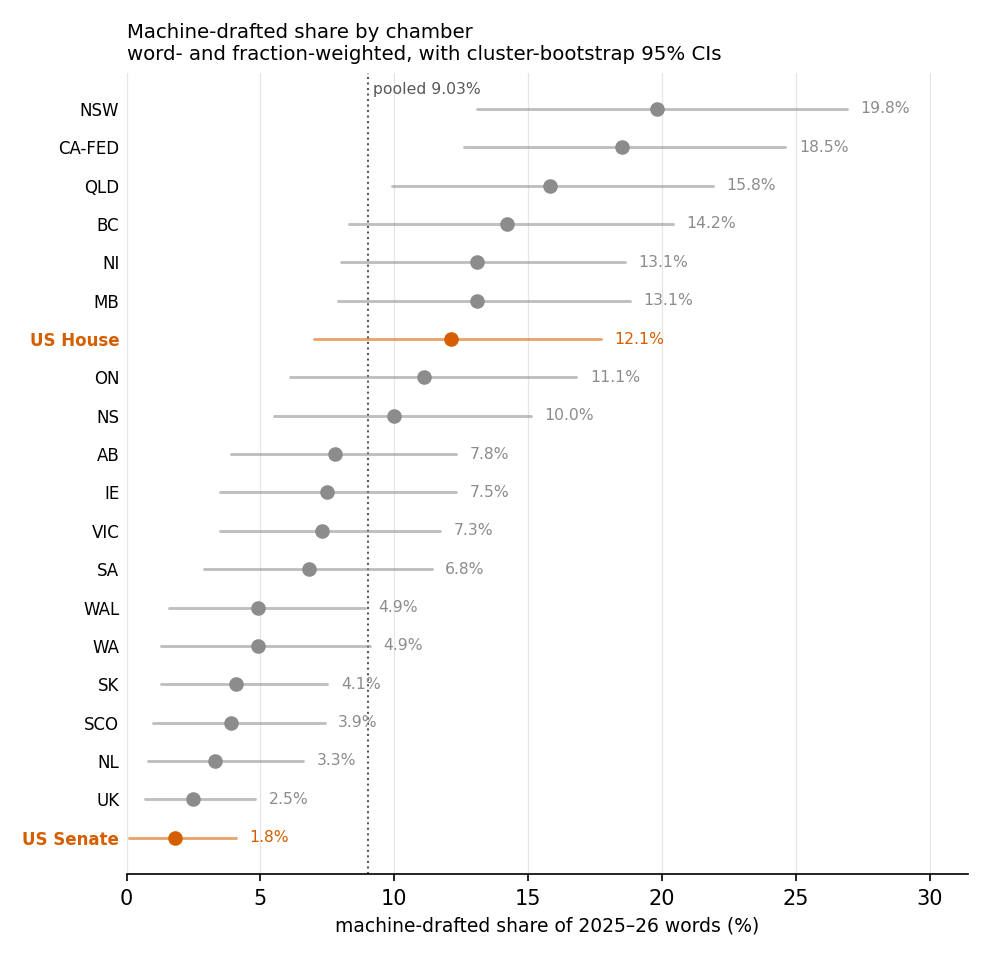
\includegraphics[width=0.85\linewidth]{chamber_prevalence_dotplot.png}
\caption{The twenty chamber rates, drawn: each point is the chamber\textquotesingle s word-weighted, fraction-weighted machine-drafted share of 2025--26 words (values exactly as in \cref{tab:prevalence}); whiskers are the cluster-bootstrap 95\% CIs; chambers sorted by rate, direct-labelled, with the two US chambers emphasised and the pooled 9.03\% marked as a reference line. Axis starts at zero.}
\label{fig:prevalence-dots}
\end{figure}

Intervals are cluster bootstraps over segments, not Wilson intervals: the
estimator is a ratio of two random sums whose numerator and denominator move
together, so a chamber whose one flagged segment happens to run 900 words
should read as less certain than one whose flag is 130 words, and a binomial on
segment counts cannot express that.\footnote{\texttt{python\ -\allowbreak{}c\ "import\ banded\_\allowbreak{}prevalence\ as\ B;\ B.\allowbreak{}table(B.\allowbreak{}load())"}.} One further honesty about the
low rows: a single 60/60 control\textquotesingle s Wilson lower bound is 94\%, so no
chamber\textquotesingle s rate below \textasciitilde6\% is calibration-exact on its own control alone;
under the pooled floor (\(\geq\)99.7\%) at most 0.3 points of any chamber\textquotesingle s rate
could be false positives --- slack that matters only for the lowest rows
(US Senate 1.8\%, UK 2.5\%) and not for the spread.

The spread is the finding, not noise around a mean. A random-effects fit
across the twenty chambers (logit-scale \(\tau\) = 0.56, I\({}^{2}\) = 0.78 --- 78\% of the
observed between-chamber variance is true heterogeneity, not sampling
noise) puts the chambers\textquotesingle{} rates at \textbf{4.3\% to 18.3\%, a better-than-fourfold
range}, after every chamber is pulled toward the pool in proportion to
its own noise. The per-chamber table reports the raw estimates; the
shrunken range is the honest spread claim, since the extremes of twenty
noisy cells overstate their own separation (the raw-extremes version is
retired to Appendix~\ref{app:superseded}). What drives a chamber\textquotesingle s position is not
established here --- even two chambers of one legislature can sit far apart
(Appendix~\ref{app:future} item 7), and the study does not attribute the between-chamber differences to
any measured cause.

\textbf{Federal Canada\textquotesingle s row comes from its own uniform draw}, not from the
genre-stratified sample that answers \cref{sec:genre}. The genre arm takes 60 segments
each from Statements by Members, Government Orders and Oral Questions, which
imposes a genre mix rather than observing one and leaves 25.6\% of the chamber\textquotesingle s
in-band record --- Private Members\textquotesingle{} Business, Adjournment Proceedings, Routine
Proceedings, the Throne Speech reply --- in no stratum at all. Read as a chamber
rate it gives 16.5\%; the uniform draw of 120 prevalence segments gives \textbf{18.5\%},
and the uniform draw is what \cref{tab:prevalence} reports. Dropping CA-FED entirely leaves
the pool at 8.50\% against 9.03\%, so the chamber contributes about half a point
to the headline and neither makes nor breaks it.\footnote{\texttt{pangram\_\allowbreak{}ch\_\allowbreak{}verdicts.\allowbreak{}csv}, rows \texttt{caprev*}/\texttt{cactl*}. Its short band
  already matched this draw: \(120\times\) 15,236/18,029 = 101, and 101 short
  segments were scored at the matched rate. Seven controls dated after the
  2022-06-30 cutoff --- one of them after ChatGPT shipped --- were replaced on
  2026-08-13 from the same 2018--2022 window the survivors occupy
  (\texttt{build\_\allowbreak{}cafed\_\allowbreak{}ctl\_\allowbreak{}redraw.\allowbreak{}py}); all seven replacements scored Human, as had
  all seven originals, so specificity is unchanged at 60/60 and only the
  design claim is repaired.}

\textbf{UK Commons and Dáil Éireann are scored entirely on Pangram 4}, verified
rather than assumed: all 360 of their segments from the four-chamber arm, which
recorded no model version, were rescored through the dashboard and agree with
the original verdicts \textbf{360 out of 360}. That agreement is itself the largest
Pangram 3-versus-4 comparison in the study (\cref{sec:detector}).

\textbf{Manitoba\textquotesingle s 13.1\% depends on a repaired extractor}, and without it the
chamber reads 5.3\%. The original extraction lost 42\% of the record: from
mid-2018 the Manitoba Hansard export splits a speaker\textquotesingle s name across several bold runs
around inserted table-of-contents anchors, the extractor\textquotesingle s prefix pattern
matched only the first run, and the speech accreted to the previous turn --- the
Speaker\textquotesingle s --- where it was discarded as chair voice. Chair share of page text ran
4\% in 2011--13 against 37--40\% in 2020--24.

The loss was \textbf{not neutral}, which is why it matters so much. A frame missing
42\% of text at random would leave the rate roughly unchanged. What was
missing were the formatted, anchor-bearing speeches --- the prepared ones --- and
prepared business is exactly where drafting concentrates (\cref{sec:genre}). The extractor
was preferentially deleting the machine-drafted half of the chamber\textquotesingle s record.

The controls are the check that this is a frame effect and not the detector
behaving differently: they were clean before the fix and remain clean after,
\textbf{0 of 18,342 words}. 275 segments were redrawn from the corrected extraction
and rescored, restricted to the original year windows so that the frame is the
only thing that changed.\footnote{\texttt{python\ build\_\allowbreak{}mb\_\allowbreak{}redraw.\allowbreak{}py}, then \texttt{pangram\_\allowbreak{}mb\_\allowbreak{}redraw\_\allowbreak{}verdicts.\allowbreak{}csv}.
  The redraw deliberately excludes the years backfilled in August 2026: a
  first draw from the corrected frame pulled 30 of its 90 controls from
  2011--14 and 2020--22, years no other chamber can draw from, which would have
  confounded the frame repair with a change of window. The superseded
  extraction is kept at \texttt{provinces/superseded/} so the pre-fix verdicts stay
  reproducible --- 135 of the old 278 seg\_ids do not exist in the corrected
  file, because re-extraction shifts turn indices.}

\subsection{Drafting concentrates in scripted business}\label{sec:genre}

Machine drafting concentrates where the procedure permits advance
preparation. Federal Canada is the only corpus carrying a business rubric,
which makes the test possible at all.

The three genres form a ladder in \textbf{how much advance preparation the
procedure permits}, which is the mechanism under test:

\begin{itemize}
\tightlist
\item
  \textbf{SO31 --- Statements by Members.} Under Standing Order 31 a non-minister
  may address the House for up to one minute on any subject, immediately
  before Question Period. Not debatable, no reply. Written ahead and read.
\item
  \textbf{Government Orders.} Government bills and motions. Covers both prepared
  speeches (20 minutes for early slots, 10 later) \textbf{and the spontaneous
  questions-and-comments periods that follow each one} --- a genuinely mixed
  category, not pure prepared debate.
\item
  \textbf{Oral Questions.} The 45 minutes after SO31. \textbf{Questions are not placed
  on notice}, so neither question nor answer can be fully drafted in
  advance; both sides are held to roughly 35 seconds.
\end{itemize}

\begingroup\small
\begin{longtable}[]{@{}lll@{}}
\caption{Machine-drafted share by genre of business, 2025--26.}\label{tab:genre}\\
\toprule\noalign{}
genre, 2025--26 & flagged words & 95\% CI \\
\midrule\noalign{}
\endfirsthead
\toprule\noalign{}
genre, 2025--26 & flagged words & 95\% CI \\
\midrule\noalign{}
\endhead
\bottomrule\noalign{}
\endlastfoot
\textbf{SO31} --- one-minute scripted set-pieces & \textbf{32.3\%} & {[}21.5, 44.1{]} \\
Government Orders --- mixed prepared and spontaneous & 19.9\% & {[}10.5, 30.5{]} \\
\textbf{Oral Questions} --- not on notice & \textbf{9.8\%} & {[}2.2, 19.1{]} \\
all three pre-AI controls (0/180) & \textbf{0.0\%} & {[}0.0, 2.1{]} \\
\end{longtable}
\endgroup

\textbf{SO31 vs OQ: \(3.29\times\), +22.5pp, permutation p = 0.0025.}

Word-weighted and fraction-weighted, like every other rate here. \textbf{Weighting
by the AI share widened this ladder rather than flattening it}, which was not
the expected direction: Mixed verdicts are commoner in the mixed-format
Government Orders than in the scripted SO31 set pieces, so counting Mixed
segments as wholly machine had been flattering the middle rung. On binary
counting the three read 35.8\% / 25.7\% / 11.8\% and a \(3.03\times\) ratio.

The word-weighting choice matters more in this table than anywhere else in the
study: the genres differ sharply in how long
their segments are --- SO31 is a one-minute set piece, a Government Orders slot
runs twenty --- so a segment-weighted comparison measures the packer\textquotesingle s behaviour
across genres alongside the drafting. On segments the same data reads 36.7\% /
23.3\% / 8.3\% and a \(4.40\times\) ratio; word- and fraction-weighted the ordering is
unchanged and \textbf{the gap settles at \(3.29\times\)}. The test is a label permutation rather than
Fisher exact, because Fisher takes segment counts and the estimator is a ratio
of summed words.\footnote{\texttt{python\ prevalence\_\allowbreak{}report.\allowbreak{}py} for the rates and bootstrap intervals;
  the SO31-vs-OQ permutation is 50,000 label shuffles of the pooled
  prevalence segments. Reported here rather than the old Fisher p = 0.00034,
  which tested a quantity the study no longer reports. The same script prints
  the Cochran--Armitage trend statistic on the segment counts (doses
  OQ \textless{} DEBATE \textless{} SO31); the adjacent-rung Fisher exacts are computed from the
  \(3\times\)2 segment table.}

The ordering is exactly what the mechanism predicts --- the more preparable the
format, the more machine drafting --- and it is the one place where the lexicon
arm\textquotesingle s inference is confirmed by an independent instrument. Two instruments
agreeing is worth more than either alone.

The monotone trend across all three rungs is the ladder\textquotesingle s proper test, and it
holds: a Cochran--Armitage trend test on the segment counts (5, 14 and 22 flags
of 60) gives z = 3.70, \(p = 2.2\times 10^{-4}\).\footnote{\texttt{python\ prevalence\_\allowbreak{}report.\allowbreak{}py} for the rates and bootstrap intervals;
  the SO31-vs-OQ permutation is 50,000 label shuffles of the pooled
  prevalence segments. Reported here rather than the old Fisher p = 0.00034,
  which tested a quantity the study no longer reports. The same script prints
  the Cochran--Armitage trend statistic on the segment counts (doses
  OQ \textless{} DEBATE \textless{} SO31); the adjacent-rung Fisher exacts are computed from the
  \(3\times\)2 segment table.} The two adjacent steps are each
individually underpowered at 60 segments per cell --- SO31 vs Government Orders
p = 0.16, Government Orders vs OQ p = 0.043 by Fisher exact --- so it is the
trend across the ladder, not any single step between neighbours, that the data
establish.

\textbf{The Oral Questions cell is not Question Period, and reading its flags
individually says more than the rate does.} The 120--360-word filter retains
95.2\% of SO31 segments but only a small fraction of Oral Questions, because
QP utterances are short. What survives is the long tail: procedural and
ceremonial business filed under the QP rubric rather than question-and-answer
exchange.

Not one of the five flagged segments is spontaneous exchange.\footnote{\texttt{python\ genre\_\allowbreak{}oq\_\allowbreak{}audit.\allowbreak{}py}, which prints the five flags with their
  order-of-business headings, the control composition, and the unmet tribute
  control. It also retires an argument this section previously made --- that
  the length floor leaves "prepared ministerial answers", the sub-population
  "most likely to be machine-drafted". Both halves are false: ministerial and
  parliamentary-secretary segments flag \textbf{0 of 28}, all five flags coming
  from non-ministers, and the floor selects \emph{away} from ministers rather than
  toward them (ministerial share of Oral Questions falls 46.3\% \(\rightarrow\) 36.1\% across
  the filter; median ministerial utterance 89 words against 95). The
  conclusion that the cell is biased upward survives; that mechanism does
  not.} Two are
\textbf{eulogies} for a former member. One is a \textbf{question of privilege}
responding to a matter raised the previous day. One is a \textbf{unanimous-consent
motion} --- text negotiated between parties beforehand and read verbatim, the
most pre-written thing that happens in the chamber. The fifth is a backbench
question of the routinely staff-written kind. The genre claim therefore holds
segment by segment and not only in aggregate: within the genre nominated as
unscripted, the flags land exactly on the parts that were written in advance.

This makes the Oral Questions rate a \textbf{mislabelled row rather than a wrong one} --- 9.8\% word-weighted in \cref{tab:genre}, 8.3\% on segments. It is not an estimate of Question Period; it is an estimate of long-tail business carrying the QP heading, and the true rate for genuine exchange is lower --- possibly zero.

\textbf{One flag type has no control, and it should not be leaned on.} Two of the
five are tributes, both at \texttt{fraction\_ai} 1.0, and \textbf{no pre-AI tribute exists
anywhere in the control set}. Tribute register --- elevated, cadenced, parallel
construction, abstract virtue nouns --- is exactly what a detector keys on. Those
two are either strong evidence of drafting or the most interesting false
positive in the study, and nothing here separates the two readings. What the
controls do establish is that formal prepared \emph{procedural} speech does not trip
the detector: the six pre-AI privilege and Business-of-the-House segments among
the CA-FED controls all read Human, inside the 1,260/1,260 overall.

Extraction is paragraph-level throughout, so no genre loses whole speeches to
the length cap; the differential retention above is a property of natural
utterance length, not of truncation. Flag rate itself rises with segment length
(\cref{sec:limits}), which cuts the same way: the filter keeps Oral Questions\textquotesingle{} longer segments,
so the surviving cell is biased \emph{up}, and true Question-Period exchange sits
lower still.

\subsection{The Opus screen tracks Pangram}\label{sec:screen-pangram}

A blinded LLM screen over the full corpus (37,801 segments, date-blind)
separates Pangram\textquotesingle s classes cleanly on the 618-segment overlap:

\begingroup\small
\begin{longtable}[]{@{}lll@{}}
\caption{Mean Opus screen score by Pangram verdict on the 618-segment overlap.}\label{tab:screen-by-verdict}\\
\toprule\noalign{}
Pangram verdict & n & mean Opus score \\
\midrule\noalign{}
\endfirsthead
\toprule\noalign{}
Pangram verdict & n & mean Opus score \\
\midrule\noalign{}
\endhead
\bottomrule\noalign{}
\endlastfoot
AI & 78 & 50.9 \\
Mixed & 26 & 44.8 \\
Human & 514 & \textbf{11.9} \\
\end{longtable}
\endgroup

The deployed screen --- the run over all 37,801 segments --- separates Pangram\textquotesingle s
AI and human classes at \textbf{AUC 0.954} {[}0.934, 0.971{]} on the 618-segment
overlap, and it is a cheap stratifier for future work.\footnote{\texttt{python\ opus\_\allowbreak{}screen\_\allowbreak{}auc.\allowbreak{}py}. The deployed screen is
  \texttt{opus\_screen\_full.js} (473 batches of 40), distinct from the lean
  validation run used in the effort A/B below; the two differ in score level
  (mean 34.3 vs 26.5) but not in discrimination. All labels are Pangram 4.} The pool is a
case-control mixture whose human class is drawn partly from pre-2023 text,
which is \emph{provably} pre-LLM and therefore the cleanest available negative;
restricting the negatives to 2023-and-later contemporary speech only \emph{lowers}
the AUC, to \textbf{0.940} {[}0.915, 0.961{]}. Contemporary human speech is the harder
class to separate --- as the permeation finding (\cref{sec:permeation}) predicts --- so the era mix is not
flattering the screen.

\textbf{Reasoning effort buys nothing here, and that is worth stating rather than
hiding.} The screen was tuned and validated at \texttt{effort=low}, and low had
never been compared against anything. Re-run on the 241-segment labelled pool
with the prompt and batching held byte-identical (all AUCs against Pangram 4):

\begingroup\small
\begin{longtable}[]{@{}lll@{}}
\caption{Agreement of the Opus screen with Pangram across runs (AUC).}\label{tab:screen-auc}\\
\toprule\noalign{}
run & AUC & 95\% CI \\
\midrule\noalign{}
\endfirsthead
\toprule\noalign{}
run & AUC & 95\% CI \\
\midrule\noalign{}
\endhead
\bottomrule\noalign{}
\endlastfoot
archived low & 0.948 & {[}0.920, 0.973{]} \\
fresh low (replicate) & 0.951 & {[}0.923, 0.974{]} \\
\textbf{max} & \textbf{0.942} & {[}0.911, 0.968{]} \\
\end{longtable}
\endgroup

The low-effort run was replicated so the effort comparison has a noise floor.
A paired bootstrap of max \(-\) mean(low) gives \textbf{\(-0.007\)}, 95\% CI
\textbf{{[}\(-0.023\), +0.007{]}}: centred below zero, and the whole interval sits below
even the +0.015 the weaker open model gains from reasoning, let alone Qwen\textquotesingle s
+0.172. Effects below \textasciitilde0.03 AUC are outside this design\textquotesingle s resolution.
Per-segment correlations agree: low-vs-low r = +0.976, low-vs-max +0.959 and
+0.960 --- max ranks the same and is \emph{more decisive on the human class} (it
sends more clear negatives to the floor), not a different scorer.

Against a single low run, max would have looked like a small decline and been
tempting to report as an effect. \textbf{The replicate is what makes the null
readable.}

This also cuts against the pattern in the open models, measured on the same
pool: effort moved Qwen3-32B by \textbf{+0.172} and gpt-oss-120b by \textbf{+0.015},
against \textbf{\(-0.007\)} for Opus. Reasoning closes part of the gap for weak
detectors and does nothing for a strong one --- and the sharper point is that
the frontier model is not reasoning its way to 0.95; it is recognising
something at a glance. Practically, the screen can be run for about \textbf{\(4\times\) fewer reasoning
tokens (\textasciitilde\(2\times\) all-in)} with no loss --- a saving observed in the run logs rather than recorded in the committed AUC artifacts.\footnote{\texttt{opus\_effort\_ab.py}, \texttt{opus\_effort\_ab.csv}.}

\subsection{The register shift starts in 1994--96, decades before the machines}\label{sec:register-shift}

The register\textquotesingle s rise begins around \textbf{1994--96} --- before the consumer web,
and long before any language model. The dated onset is a property of the
one series that reaches behind it: UK Commons extended back to 1985, where
the register \emph{declines} through the late 1980s before turning upward at
that window (only three chambers reach 1994 at all; the cross-chamber
evidence for the drift itself is the nineteen-chamber comparison of
\cref{sec:climb-geography}). Whatever this measures, LLMs did not start it.\footnote{\texttt{python\ long\_\allowbreak{}trend.\allowbreak{}py\ -\allowbreak{}\/\allowbreak{}-\allowbreak{}seg\ uk/\allowbreak{}segments\_\allowbreak{}uk\_\allowbreak{}deep.\allowbreak{}jsonl} for the annual
  series; the turning point is the minimum of the annual
  instrument-minus-placebo gap (the script fits no curve), and it lands on
  1994. A day-clustered bootstrap (\texttt{python\ long\_\allowbreak{}trend\_\allowbreak{}bootstrap.\allowbreak{}py}, 2,000
  resamples of sitting days within year) puts the minimum at 1994 in 84.8\% of
  resamples, 1995 in 13.0\% and 1996 in 2.1\% --- so "1994--96" is a genuine
  {[}1994, 1996{]} interval, not a hedge.}

\textbf{The register instrument is not a detector, and a direct test is why the
roles are divided.} A simple threshold on the register score --- the study\textquotesingle s
own 407-word occurrence rate --- separates Pangram-flagged from unflagged
legislative segments at \textbf{AUC 0.61} (0.60 restricted to the 2025--26
prevalence sample, where both classes are drifted contemporary speech),
against the screen\textquotesingle s 0.95. On ground truth it does no better: \textbf{0.535}
against known machine text --- though that set is the evasion run\textquotesingle s
adversarially quietened rewrites rather than ordinary model output, which
runs far hotter on these words (\cref{sec:posttraining}). One thin lexical rate carries
population-level history well and instance-level detection barely above
chance, which is the division of labour the study uses.\footnote{\texttt{python\ register\_\allowbreak{}auc\_\allowbreak{}check.\allowbreak{}py}: 5,439 text-resolved
  Pangram-scored legislative segments (prevalence, controls, the genre
  arm) plus the 292 final-run bypass variants; AUC by Mann--Whitney.
  Everything pooled: 0.57. Medians per 100k: controls 3,150; unflagged
  2025--26 prevalence 3,226; flagged 3,869; LLM variants 3,327.}

\textbf{The ruler, audited --- what the thirty-year rise is made of.} Selected on the post-2022 jump and run backwards, the marker list invites two objections --- that the rise is a few words, and that a list selected on an endpoint would trend by construction --- so both were tested.\footnote{\texttt{python\ build\_\allowbreak{}word\_\allowbreak{}year\_\allowbreak{}counts.\allowbreak{}py} (one scan, 1.62B tokens;
  reproduces the committed series to 0.00 per 100k at the worst year)
  then \texttt{python\ ruler\_audit.py}, \texttt{python\ donor\_series.py} (trend-matched
  donors, 389/407 matched, 99.7\% exact on all three deciles; the
  freq+dispersion variant is \texttt{donor\_series\_fc.json}) and
  \texttt{python\ length\_\allowbreak{}poststrat.\allowbreak{}py}. The audit also caught a defect in the
  committed placebo builder: its top-120-frequency exclusion leaves
  eight style words --- \texttt{this} among them --- matched far below their own
  frequency; the donor pool here does not exclude them.} The rise is concentrated: \textbf{ten common connectives carry 92.5\% of the 1994--96 \(\rightarrow\) 2024--26 climb} (\texttt{this} alone 35\%), and with those ten removed the aggregate is nearly flat (\(\times\)1.03 pooled, \(\times\)1.10 UK). What rises beneath them is \textbf{breadth}: the expected distinct style words per 1,000 tokens climbs \(\times\)1.26 on the UK series (14.4 \(\rightarrow\) 18.2), and 60.4\% of the 407 words trend positive (z = +4.2) at a median of only +0.5\%/yr --- a shallow, broad widening under a few surging function words, not a 407-word chorus.

The rise is not a composition artifact: post-stratifying every chamber-year to a fixed segment-length distribution --- the measurable proxy for the genre drift \cref{sec:genre} makes threatening --- leaves the onset in place and slightly \emph{strengthens} the UK climb (\(\times\)1.49 \(\rightarrow\) \(\times\)1.54). It is not a one-ruler artifact either: the independent Wikipedia signs-of-AI-writing patterns, built by different people for a different purpose, rise across the whole pre-LLM record and \emph{faster} (+2.7\%/yr against +1.4\%/yr, UK 1994--2019) --- though their UK trough sits in 1987, so the decades-long pre-LLM rise is a cross-instrument fact while the specific 1994--96 date belongs to this ruler\textquotesingle s UK series.

Against donors matched on frequency and dispersion, the UK series\textquotesingle{} interior minimum at 1994 survives; matched additionally on pre-2010 trend --- a control that by construction absorbs any onset inside its own window --- the register\textquotesingle s \emph{distinctive} excess over ordinary same-shaped vocabulary dates to roughly \textbf{2014--2018}, and the style words sit below their matched donors in level for the entire record until 2025. The drift is real, broad-based, composition-robust and instrument-robust; its dated 1994--96 turn is the UK ruler\textquotesingle s; and its excess over matched controls is younger than the turn.

Read together with \cref{sec:posttraining}, the interesting reading is not "LLMs changed
parliamentary register" but that \textbf{human register had been moving toward what
instruct-tuning later selected for, for thirty years.} †\footnote{Daggered numbers are carried from earlier in the study and were
  re-derived from their artifacts; the full key and per-number sources are
  in the Supplementary provenance note.}

The machines then accelerated it, and left a fingerprint of their own suppression. In New Brunswick --- the one corpus sampled densely enough to resolve quarters --- an interrupted time series with the break pre-set at ChatGPT\textquotesingle s release finds a flat pre-2023 slope (\(-1.2\)\%/yr) turning to \textbf{+23.7\%/yr} afterward, significant against 1,000 frequency-matched placebo word sets (p = 0.007; Mann--Kendall\cite{mann1945,kendall1948} p = 0.014).

But the two instruments then part ways (\cref{fig:trend}): the \emph{obvious} tells --- the Wikipedia "signs of AI writing" set --- peak around 2025 and fall back, while the subtler Kobak rare-style set keeps climbing. The natural reading --- with published precedent in scholarly text, where Gray\cite{gray2025} documents distinctive marker words dropping in frequency once publicised --- is that the conspicuous words became notorious and were trained or edited away, while the register underneath kept rising. The peak-and-fall of the obvious tells shows in some other chambers too --- UK Commons and the US House both turn down after 2024 --- though it is not universal (Ireland\textquotesingle s keep rising), so this is a suggestive cross-chamber pattern rather than a law; the clean two-instrument contrast is sharpest in the densely-sampled discovery corpus.\footnote{\texttt{python\ fig\_trend.py} for New Brunswick --- the interrupted time series is weighted least squares on log quarterly rates with a break pre-specified at 2023.0, and the empirical p for the slope change comes from 1,000 frequency-matched placebo word sets run through the identical fit. The cross-chamber comparison is \texttt{python\ build\_\allowbreak{}trend\_\allowbreak{}cache.\allowbreak{}py\ \&\&\ python\ plot\_\allowbreak{}trend\_\allowbreak{}from\_\allowbreak{}cache.\allowbreak{}py}; indexed yearly rates for six chambers are in \texttt{trend\_multichamber.csv}.}

\begin{figure}[htbp]
\centering
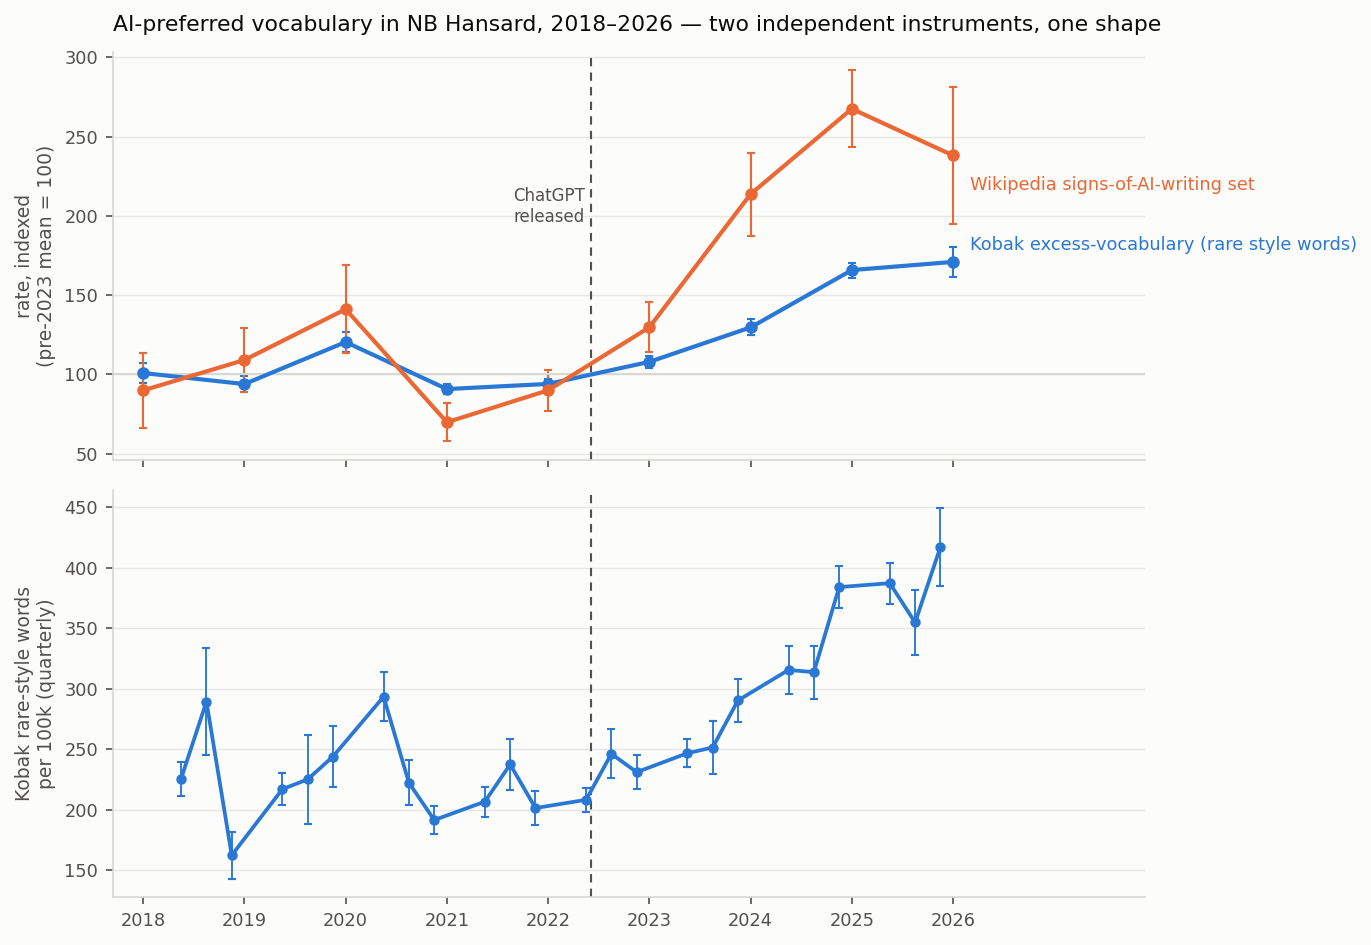
\includegraphics[width=0.85\linewidth]{the-ai-lexicon-trend.png}
\caption{The recent acceleration, New Brunswick Hansard. Panel A: yearly rates on both instruments --- the Wikipedia "signs of AI writing" set and Kobak rare-style words --- each indexed to its own pre-2023 mean = 100. The obvious tells peak around 2025 and fall back; the subtler set keeps climbing. Panel B: the quarterly Kobak rare-style rate per 100k with Poisson 95\% whiskers, ChatGPT\textquotesingle s release marked and the interrupted-time-series break set there. The decades-long rise established above predates this jump.}
\label{fig:trend}
\end{figure}

\subsection{Other chambers converge on the level the United States already held}\label{sec:climb-geography}

Running the same series on every chamber turns the thirty-year drift into a
comparison. The instrument and the 200 matched placebo sets are built once, on
UK Commons 2010--12, and applied unchanged everywhere, so the chambers are
measured with the same ruler.\footnote{\texttt{python\ occurrence\_\allowbreak{}trends.\allowbreak{}py\ -\allowbreak{}\/\allowbreak{}-\allowbreak{}build\ -\allowbreak{}\/\allowbreak{}-\allowbreak{}report}. Word-weighted, pooled
  into fixed-composition panels; a pooled line whose membership changes
  between years is a picture of the download schedule, not a trend. Chamber
  coverage and every gap are tabulated in the output. 2023 is missing from
  most chambers because the study design excluded it as a washout year
  between the 2018--22 and 2024--26 windows.}

\Cref{fig:convergence} draws it: nineteen chambers hold both endpoints of the longest window most of the
corpus shares --- 2006 to 2026 --- and on that single ruler the pattern is
convergence: \textbf{the lower a chamber started, the faster it climbed} (Spearman
between 2006 level and growth \(-0.56\), n = 19; taking the baseline from
2006--08 means and measuring growth on the disjoint 2010--2026 span --- the
split that removes regression-to-the-mean coupling --- gives \(-0.51\), n = 18).
And the convergence sits on a shared direction, not a see-saw: sixteen of
the nineteen chambers rise on the constant window. The four lowest 2006 starters ---
UK Commons, Scotland, Northern Ireland, Wales --- are the four fastest
climbers; only three chambers decline at all (US House, US Senate, Prince
Edward Island), and none of the nineteen approaches the UK\textquotesingle s +4.0\%/yr.\footnote{\texttt{python\ constant\_\allowbreak{}window\_\allowbreak{}trend.\allowbreak{}py}, reading
  \texttt{occurrence\_trends.json}; endpoints 2006 and 2026, growth as the
  geometric rate over the twenty years. South Australia is excluded for
  missing the 2026 endpoint (its series ends 2025); Ireland and federal
  Canada for entering late. Tasmania carries \cref{sec:prevalence}\textquotesingle s regime flag; its row
  is descriptive.}

\begingroup\small
\begin{longtable}[]{@{}lllll@{}}
\caption{The constant-window register trend: nineteen chambers, 2006--2026, ordered by growth.}\label{tab:climb}\\
\toprule\noalign{}
chamber & gap 2006 & gap 2026 & change & per year \\
\midrule\noalign{}
\endfirsthead
\toprule\noalign{}
chamber & gap 2006 & gap 2026 & change & per year \\
\midrule\noalign{}
\endhead
\bottomrule\noalign{}
\endlastfoot
UK Commons & 655 & 1,444 & \(\times\)2.20 & \textbf{+4.0\%/yr} \\
Scotland & 605 & 1,058 & \(\times\)1.75 & +2.8\%/yr \\
Northern Ireland & 739 & 1,165 & \(\times\)1.58 & +2.3\%/yr \\
Wales & 1,276 & 1,961 & \(\times\)1.54 & +2.2\%/yr \\
Saskatchewan & 1,612 & 2,145 & \(\times\)1.33 & +1.4\%/yr \\
British Columbia & 1,542 & 2,049 & \(\times\)1.33 & +1.4\%/yr \\
Manitoba & 1,636 & 2,136 & \(\times\)1.31 & +1.3\%/yr \\
Western Australia & 1,366 & 1,751 & \(\times\)1.28 & +1.3\%/yr \\
Victoria & 1,619 & 2,043 & \(\times\)1.26 & +1.2\%/yr \\
Queensland & 1,746 & 2,199 & \(\times\)1.26 & +1.2\%/yr \\
Tasmania & 1,631 & 2,049 & \(\times\)1.26 & +1.1\%/yr \\
Nova Scotia & 1,811 & 2,265 & \(\times\)1.25 & +1.1\%/yr \\
New South Wales & 1,276 & 1,593 & \(\times\)1.25 & +1.1\%/yr \\
Alberta & 1,746 & 2,125 & \(\times\)1.22 & +1.0\%/yr \\
Ontario & 1,707 & 2,013 & \(\times\)1.18 & +0.8\%/yr \\
Newfoundland \& Labrador & 1,436 & 1,532 & \(\times\)1.07 & +0.3\%/yr \\
\textbf{US Senate} & 1,590 & 1,562 & \(\times\)0.98 & \(-0.1\)\%/yr \\
Prince Edward Island & 1,589 & 1,523 & \(\times\)0.96 & \(-0.2\)\%/yr \\
\textbf{US House} & 1,794 & 1,709 & \(\times\)0.95 & \(-0.2\)\%/yr \\
\end{longtable}
\endgroup

\begin{figure}[htbp]
\centering
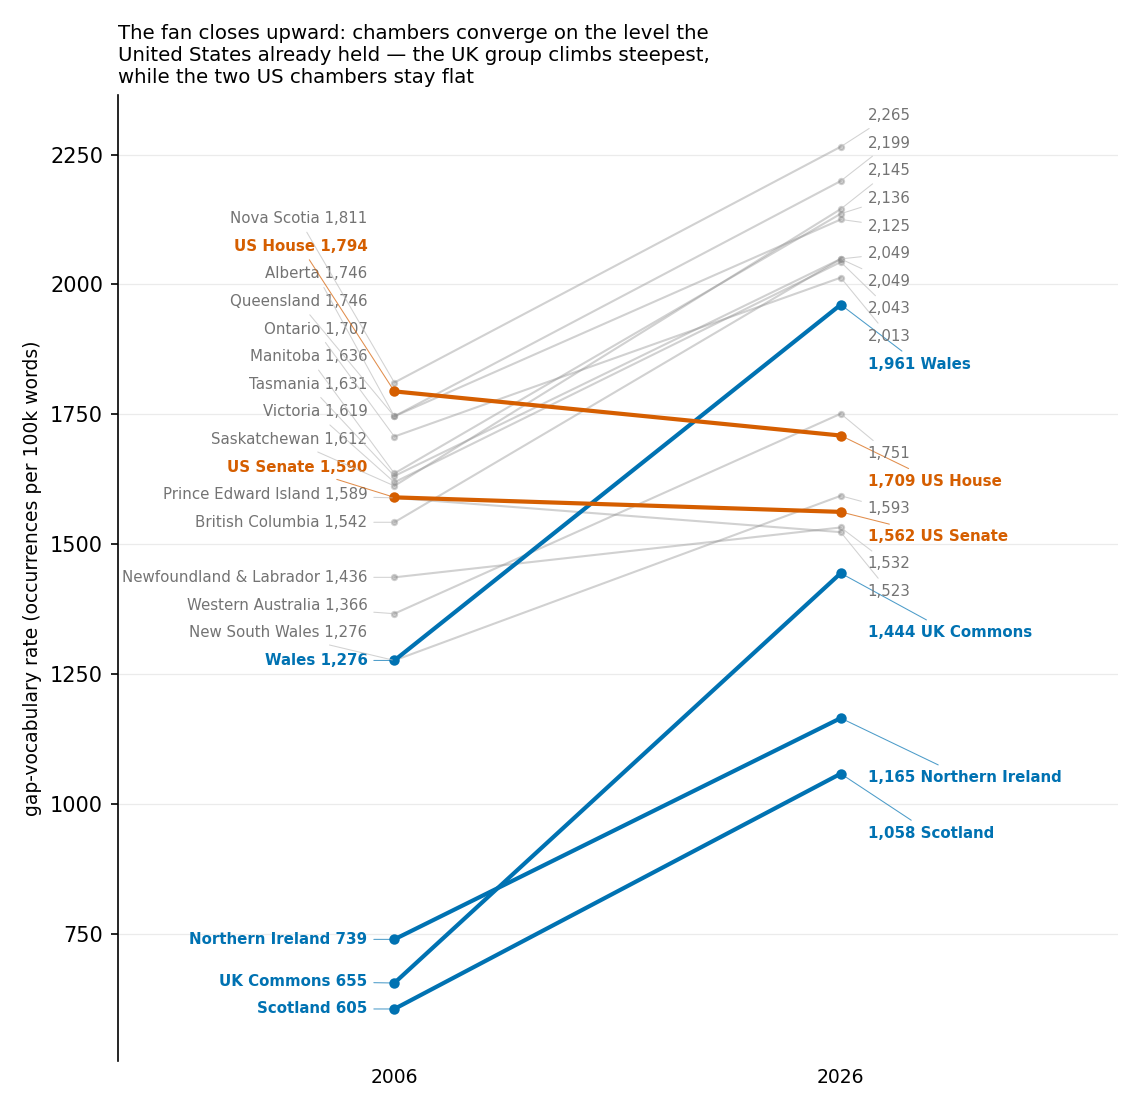
\includegraphics[width=0.85\linewidth]{convergence_slopegraph.png}
\caption{The convergence, drawn as a slopegraph: one line per chamber from its 2006 to its 2026 gap-vocabulary rate (occurrences per 100k words; values exactly as in \cref{tab:climb}), direct-labelled at both ends, the UK-group climbers and the two flat US chambers emphasised. The fan closes upward: the lowest 2006 starters climb steepest toward the level the United States already held.}
\label{fig:convergence}
\end{figure}

Three chambers reach further back, and the US point rests on that longer
window:

\begingroup\small
\begin{longtable}[]{@{}lllll@{}}
\caption{The longest window: the three chambers whose series reach 1994.}\label{tab:climb-long}\\
\toprule\noalign{}
chamber & gap 1994 & gap 2026 & change & per year \\
\midrule\noalign{}
\endfirsthead
\toprule\noalign{}
chamber & gap 1994 & gap 2026 & change & per year \\
\midrule\noalign{}
\endhead
\bottomrule\noalign{}
\endlastfoot
UK Commons & 380 & \textbf{1,444} & \textbf{\(\times\)3.80} & \textbf{+4.3\%/yr} \\
\textbf{US House} & \textbf{1,515} & 1,709 & \(\times\)1.13 & +0.4\%/yr \\
\textbf{US Senate} & \textbf{1,314} & 1,562 & \(\times\)1.19 & +0.5\%/yr \\
\end{longtable}
\endgroup

Only the UK and the two US chambers hold 1994 (the UK\textquotesingle s own series extends
to 1985, \cref{sec:register-shift}), and on that longest window the contrast sharpens --- with the
US chambers \emph{starting} above where the UK still sits two decades later, US
House at 1,515 per 100k in 1994 against the UK\textquotesingle s 1,444 in 2026. Ireland and
federal Canada, excluded from both tables for entering late (2018, 2015),
enter high --- 1,603 and 1,865 --- and move like chambers already near the
ceiling (+2.6\%/yr and \(-0.7\)\%/yr). So the picture is not a common shift. It is
chambers converging upward on a level the United States already held before
the consumer web, while the United States barely moves.

A US series that starts in 2006 cannot distinguish "the United States was always there" from "the United States got there first and stopped." Extending the Congressional Record to its 1994 beginning settles it.\footnote{\texttt{python\ us/\allowbreak{}fetch\_\allowbreak{}us\_\allowbreak{}hist.\allowbreak{}py\ -\allowbreak{}\/\allowbreak{}-\allowbreak{}years\ 1994-\allowbreak{}2005,2023\ -\allowbreak{}\/\allowbreak{}-\allowbreak{}per-\allowbreak{}year\ 60\ -\allowbreak{}\/\allowbreak{}-\allowbreak{}tag\ US\_\allowbreak{}DEEP\_\allowbreak{}DONE}, then re-extract with \texttt{us/\allowbreak{}us\_\allowbreak{}extract.\allowbreak{}py\ zips\ segments\_\allowbreak{}us.\allowbreak{}jsonl} and rebuild. 780 sitting-day zips at 60 days/year;
  both chambers are now unbroken 1994-2026 with no missing year. The
  extraction nearly doubled the US corpus --- House 66.0M to 108.2M words,
  Senate 74.4M to 144.7M. Rates are per 100k words, so uniform within-year
  sampling costs precision and not validity.}

\textbf{They caught up; they did not pass.} A single recent year appears to
contradict that: in 2026 the Canadian provinces, Ireland, the Australian states
and federal Canada all sit above US House. The comparison does not survive
contact with the variance. US House swings between 1,660 and 2,074 across the
series --- a 25\% range, the widest here --- and 2026 catches it at 1,709, near its
own floor. On 2020--26 means, with each series\textquotesingle{} standard deviation alongside:

\begingroup\small
\begin{longtable}[]{@{}llll@{}}
\caption{Register level by chamber, 2020--26 means, benchmarked against the US House.}\label{tab:vs-ushouse}\\
\toprule\noalign{}
& mean & sd & vs US House \\
\midrule\noalign{}
\endfirsthead
\toprule\noalign{}
& mean & sd & vs US House \\
\midrule\noalign{}
\endhead
\bottomrule\noalign{}
\endlastfoot
CA provinces & 2,054 & 61 & \textbf{+155 (+1.28 sd)} \\
Ireland & 1,901 & 52 & +2 (+0.02 sd) \\
\textbf{US House} & \textbf{1,899} & \textbf{121} & --- \\
AUS states & 1,861 & 36 & \(-39\) (\(-0.32\) sd) \\
CA federal & 1,816 & 134 & \(-84\) (\(-0.69\) sd) \\
US Senate & 1,591 & 60 & \(-309\) (\(-2.55\) sd) \\
UK Commons & 1,415 & 61 & \(-484\) (\(-4.00\) sd) \\
\end{longtable}
\endgroup

Only the Canadian provinces are meaningfully above, and they are a standing
exception this study does not explain. Ireland is at parity to within a
fiftieth of a standard deviation; the Australian states and federal Canada are
below. Three of the four apparent overshoots are US House having a low year.

\textbf{Exported machine text does not account for the rest, and cuts the wrong
way.} The natural rescue --- that AI drafting, American-inflected, is pushing
the others past --- fails on the arithmetic: US House is \textbf{14.3\% machine by
instrument occurrences} against Ireland\textquotesingle s 9.0\% and the Australian states\textquotesingle{}
11.3\%, so removing machine text lowers the American benchmark by more than it
lowers the challengers. Federal Canada is the one case it does explain, at
21.7\% the most machine-written of the national chambers (second only to New South Wales, \cref{sec:prevalence}), dropping from
apparently-above to clearly-below once corrected.\footnote{\texttt{python\ convergence\_\allowbreak{}check.\allowbreak{}py}, with shares from
  \texttt{ai\_\allowbreak{}share\_\allowbreak{}of\_\allowbreak{}instrument.\allowbreak{}py}. Machine-written text carries the instrument at
  4,231 occurrences per 100k words against human text\textquotesingle s 3,470, a ratio of
  \(1.22\times\), so a chamber that is 9.0\% machine by words is 10.6\% machine by
  occurrences. Note this is an overlap between two instruments and not a
  causal decomposition: a high instrument rate inside flagged text is part of
  why the detector flagged it. The correction also applies only to 2025--26,
  the detector\textquotesingle s window, so it is anachronistically absent from 2023--24 where
  some machine text certainly exists unmeasured.}

\subsection{Post-training aligns weakly with pre-model American usage}\label{sec:american-alignment}

\textbf{What post-training does resembles what already distinguished American
usage.} If the two processes select for the same thing, the vocabulary shift
instruct-tuning induces should line up with the difference that already
separated American from British legislative speech before any model existed.
Measured on 4,823 words in a 2006--10 window, it does, weakly and
specifically:\footnote{\texttt{python\ alignment\_\allowbreak{}vs\_\allowbreak{}american.\allowbreak{}py}. Three families at 1,600 prompts;
  reference corpora US 37.6M, UK 44.2M, CA 74.8M, AU 88.8M words over
  2006--10 --- pre-transformer, and early enough that the UK\textquotesingle s own climb has
  barely begun, so the ratio compares two human traditions rather than two
  stages of one drift. Reported on all words. US/UK spelling pairs and
  one-word orthographic forms (\texttt{percent} for "per cent") are reported as a
  separate stratum, along with two harsher filters, as robustness only.}

\begingroup\small
\begin{longtable}[]{@{}lll@{}}
\caption{Chase-and-flight correlations, raw and holding word frequency fixed.}\label{tab:flight-corr}\\
\toprule\noalign{}
contrast & Spearman & partial, holding frequency \\
\midrule\noalign{}
\endfirsthead
\toprule\noalign{}
contrast & Spearman & partial, holding frequency \\
\midrule\noalign{}
\endhead
\bottomrule\noalign{}
\endlastfoot
post-training preference vs log(US/UK) & \textbf{+0.081} & \textbf{+0.086} \\
vs log(Canada/UK) & +0.012 & +0.012 \\
vs log(Australia/UK) & +0.018 & +0.004 \\
vs log(US/Canada) & +0.083 & +0.088 \\
\end{longtable}
\endgroup

Permutation p \textless{} 0.005. The \textbf{discrimination} carries more than the coefficient:
Canada and Australia are anglophone parliamentary democracies too, and
post-training moves models toward none of what distinguishes \emph{them} from
Westminster. It is not drift away from British usage; it is drift toward
American usage specifically, and Canada --- nearest neighbour to the United
States --- shows nothing.

The effect is small: r = 0.081 is under one percent of variance. And the design
establishes compatibility, not cause. A shared cause predicts the same
correlation --- both the models and the global drift could be downstream of an
American-dominated written corpus, with no common optimization involved. Appendix~\ref{app:future}
names the instrument that would separate those two.

\subsection{The register signal fires in every chamber, and it is not formality}\label{sec:register-robust}

The climb has a floor. Even in the chambers that are flat over time, the register is strongly present in \emph{level}: applied against each chamber\textquotesingle s own pre-2022 counterfactual, the machine-overused vocabulary is elevated in every confirmatory chamber, and Fisher\textquotesingle s method\cite{fisher1925} over the 47 corpus specifications combines to \textbf{\(p \approx 1.3\times 10^{-83}\)} (the discovery corpus, New Brunswick, is held out and reported separately, at excess +0.55). The effect is not a relabelling of formality: where a data-defined formality control exists --- Ireland, federal Canada, the UK --- the register excess exceeds the formality gap in every case (for instance UK Commons +0.26 against +0.09). The instrument measures something more specific than "this chamber speaks formally."\footnote{\texttt{python\ cross\_corpus.py}, reading each chamber\textquotesingle s frozen \texttt{*\_protocol.json} and \texttt{*\_formality.json}; Fisher\textquotesingle s method combines the per-corpus p-values over the confirmatory corpora only, per \texttt{replication\_protocol.md}. The discovery corpus is excluded from the combination and reported separately.}

\subsection{Birth year predicts the register: decomposing a juniority gradient across space and time}\label{sec:generational}

Every member-year of speech carries two clocks --- the year the words were \textbf{spoken} and the speaker\textquotesingle s \textbf{birth year} --- and birth predicts the register net of calendar time. Regressing the member-year rate on both together with chamber fixed effects, across all 22 chambers (60,186 member-years, 6,913 members): birth \textbf{+0.86 per 1,000 words per decade} (t = 14.7 clustered on member, 31.9 on raw member-years) against spoken year \textbf{+1.26} (t = 13.4 clustered). A legislator born a decade later uses about +0.86/1,000 more of the register in the same year and chamber; on identical rows the within-chamber correlation is marginally higher with birth (+0.325) than with spoken year (+0.302), and birth is the stronger of the two in 15 of the 22 chambers. †\footnote{\texttt{python\ cohort\_\allowbreak{}vs\_\allowbreak{}period.\allowbreak{}py}. The headline pair is the two-stamp fit: member-year register rate on spoken year and birth year together, chamber fixed effects, word-weighted, with errors both ways --- member-year HC, and clustered on member, the honest form since member-years are repeated draws of the same 6,913 people. All 22 chambers carry member birth years (60,186 member-years after tier-1 keys flagged ambiguous --- two members sharing a surname --- are excluded from the birth join, a filter added 2026-08-26 that also removed 49 impossible-age rows); within-chamber correlations are on the same rows. The script\textquotesingle s three-stamp fit adds entry year --- a second cohort clock, not a confounder --- and it splits the cohort credit rather than removing it (birth +0.69, t 19.3, on the 37,255 entry-censored rows); reported once here and not as the headline, because a career clock absorbing part of a birth clock is re-description, not explanation.}

That single slope is where the question starts, not where it ends. What we want from it is a \textbf{decomposition --- across space, and across time.} Across space: is one gradient shared by every legislature, or is it an average over chambers that behave differently? Across time: is "born later, uses more" about \emph{when a person was born} (cohort), \emph{what year it is} (period), or \emph{how long they have served} (career)?

The time question runs into a wall no data removes: age = year \(-\) birth, so age, period and cohort cannot be jointly separated --- a birth-plus-period model and an age-plus-period model reproduce each other\textquotesingle s fits exactly, for every number in this section. There is therefore no single conclusive estimate to report.

What there is instead is a family of \textbf{views} --- weighting members equally or by words, following people within their own careers or comparing across them, restricting to the chambers or the cohorts where one clock happens to be pinned. None settles the age/cohort split on its own; taken together they locate the gradient. The rest of this section is that family, each view named for what it is interesting for.

\textbf{Across legislatures, the individual gradient is steady where the chamber trend is not.} Group trends diverge enormously across chambers --- \(-173\) to +413 occurrences per 100k per decade --- while the within-year birth gradient sits in one narrow band (+49 to +109) in every chamber, including the two whose group trend is flat. That contrast is the low-variance signature of an individual-level effect (\cref{fig:apc}): the thing that swings wildly at the chamber level barely moves at the person level. †\footnote{\texttt{python\ apc\_\allowbreak{}chamber\_\allowbreak{}decomposition.\allowbreak{}py}, on the five chambers with exact member birth years (37k member-years, \(\geq\)2,000 words each, member-cluster bootstrap CIs); units are instrument occurrences per 100k words per decade throughout --- the same ruler as \cref{sec:climb-geography}. The all-22-chamber figures are the story-neutral accounting at birth-decade resolution; the five-chamber comparison is what separates the components.}

\textbf{Restricted to cohorts formed before the register moved, the gradient is already there.} The sharpest cell is the US Senate before any drift: among cohorts born 1917--1964, observed 1994--2004 --- every one formed decades before the register began moving anywhere --- the gradient is already full size, \textbf{+105 {[}+47, +155{]} per decade of birth}. \emph{A juniority gradient in this register predates the drift, the machines, and the web.} Read the other way round --- those cohorts\textquotesingle{} gradient IS the age profile, since cohort is pinned pre-drift --- it fixes the age slope at \textbf{\(-0.88\)/decade} (clustered t \(-3.5\)) and, propagated along the identification line (whose invariant is the same-age decade-on total, period + cohort = \textbf{+2.11/decade}), bounds the \emph{linear} cohort slope to \textbf{\(-0.03\) {[}\(-0.52\), +0.46{]}}. This view is interesting twice over: it answers "did the models create this?" (no), and as a bound it says the standing \emph{level} of the gradient reads as an age-or-career clock, not a birth-cohort one. †\footnote{\texttt{python\ apc\_\allowbreak{}solution\_\allowbreak{}line.\allowbreak{}py} (re-derives the committed two-stamp fit exactly, prints the solution line and the Senate-cell bound: n = 1,107 member-years, 160 senators, ages 31--100), \texttt{python\ apc\_i.py} (the Luo--Hodges APC-I estimator with a synthetic recovery-and-size check run first: recovery passes, and a pure-linear null yields p = 0.46, no false rejection; the aligned 5-year grouping is exactly collinear, so the reported curvature is constraint-free), and \texttt{python\ tenure\_\allowbreak{}within\_\allowbreak{}cells.\allowbreak{}py} (the between-member tenure test: \(-0.95\)/decade of tenure within birth-year \(\times\) year \(\times\) chamber cells, clustered t \(-8.3\), which is algebraically the entry-cohort term and so does not separate career stage from cohort). The identification-free contrasts are projections off the span of the linear cohort term, so they do not depend on the constraint choice.}

\textbf{The one time-statement that needs no assumption is that the cohort profile bends.} The linear age/period/cohort split is unidentifiable, but the \emph{curvature} is not, and it rejects linearity outright (Wald \(p \approx 10^{-7}\)): the constraint-invariant contrasts put cohorts born \textbf{1975 onward +0.46 above the linear profile (z = 5.1)}, those born 1985 onward +0.65 (z = 2.6), with a late-minus-early local slope difference of \textbf{+0.70/decade (z = 2.7)}. Interesting because it is the steepening claim in identification-free form, and it lands exactly where drift-formed cohorts arrive --- the register roughly tripling among them (UK Commons +30 \(\rightarrow\) +98, US House +23 \(\rightarrow\) +85, and in the House against a flat chamber mean, so if the growth is formation it is formation in the ambient written culture rather than the chamber). Its complication is stated rather than hidden: the deviation profile bends up at \emph{both} ends --- the 1920s--30s cohorts also sit above the line, on the panel\textquotesingle s thinnest cells --- so the identified fact is "nonlinear, rising at the recent end," not "rising only there." †\footnote{\texttt{python\ apc\_\allowbreak{}solution\_\allowbreak{}line.\allowbreak{}py} (re-derives the committed two-stamp fit exactly, prints the solution line and the Senate-cell bound: n = 1,107 member-years, 160 senators, ages 31--100), \texttt{python\ apc\_i.py} (the Luo--Hodges APC-I estimator with a synthetic recovery-and-size check run first: recovery passes, and a pure-linear null yields p = 0.46, no false rejection; the aligned 5-year grouping is exactly collinear, so the reported curvature is constraint-free), and \texttt{python\ tenure\_\allowbreak{}within\_\allowbreak{}cells.\allowbreak{}py} (the between-member tenure test: \(-0.95\)/decade of tenure within birth-year \(\times\) year \(\times\) chamber cells, clustered t \(-8.3\), which is algebraically the entry-cohort term and so does not separate career stage from cohort). The identification-free contrasts are projections off the span of the linear cohort term, so they do not depend on the constraint choice.}

\begin{figure}[htbp]
\centering
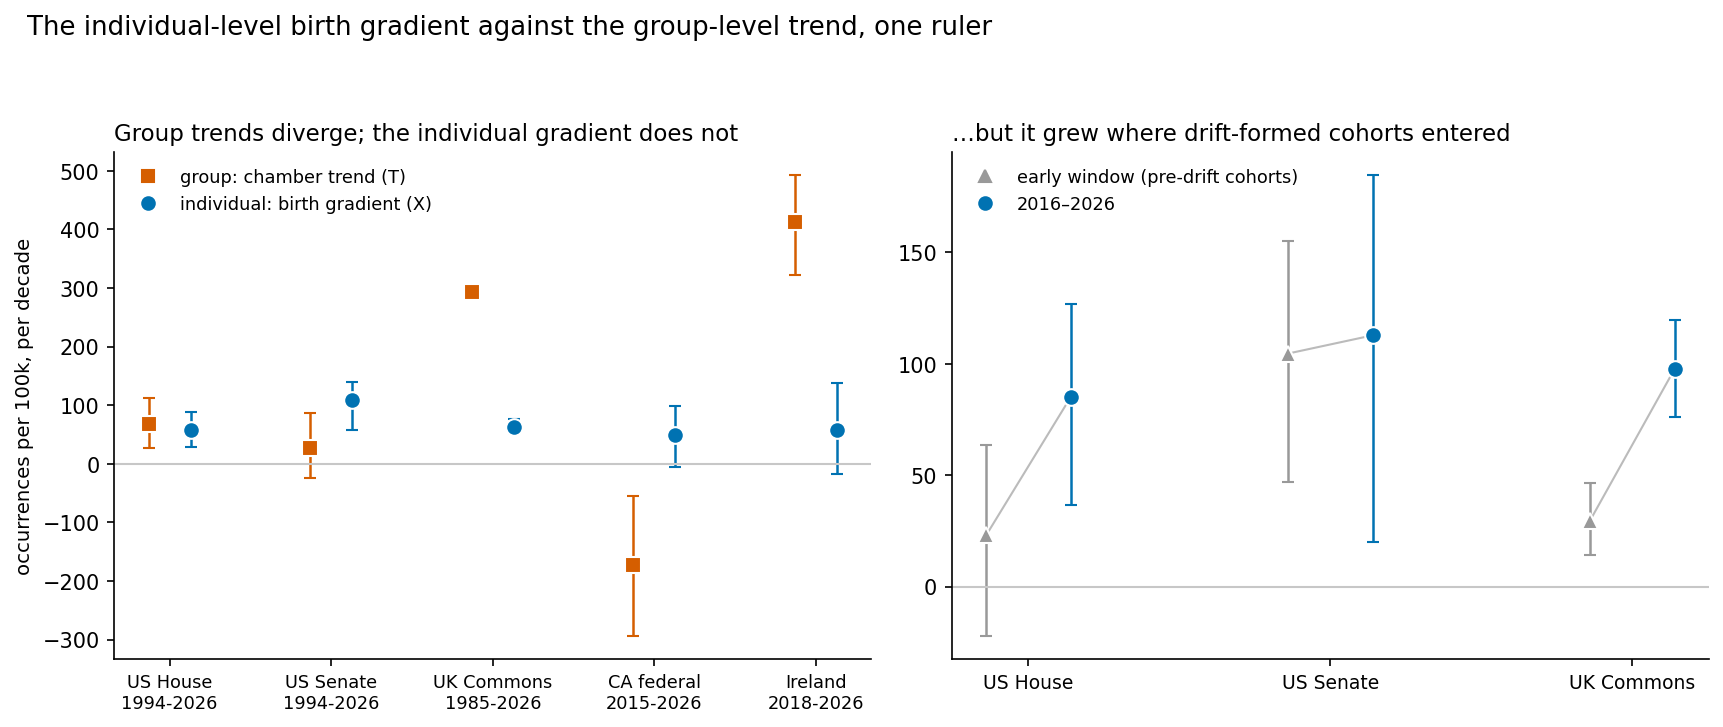
\includegraphics[width=0.85\linewidth]{apc_gradients.png}
\caption{Group-level against individual-level gradients, one ruler (instrument occurrences per 100k words, per decade). Left: chamber trends diverge across legislatures while the within-year birth gradient sits in one band --- full-size even where the trend is flat (the space view). Right: the birth gradient by era --- full-size among pre-drift cohorts in the US Senate, roughly tripling in the UK Commons and US House as drift-formed cohorts enter (the pre-drift and nonlinear views). Error bars are member-cluster bootstrap 95\% intervals.}
\label{fig:apc}
\end{figure}

\textbf{Following members over their own careers, the register rises --- but that is the calendar tide, not aging.}~(\cref{fig:tenure}) With member fixed effects, so only a member\textquotesingle s own movement counts, the register rises \textbf{+0.51 per 1,000 per decade} within member (t = 6.0, clustered on member, 8,600 members with three or more years) --- roughly \textbf{40\% of the total calendar rise happens inside continuing careers}, the rest arriving with the composition of the chamber. This view shows sitting members\textquotesingle{} rates rising, not merely that they are replaced. But it comes with a trap: within one career tenure = spoken year \(-\) entry year, so plotting register against length of service splits into two curves that cross. Within a member --- rate against their own career mean --- it \textbf{rises} with tenure (to +2.35 per 1,000 at 30+ years), which is exactly the calendar drift redrawn. Measured against same-year colleagues instead --- rate minus its chamber \(\times\) year mean --- it \textbf{falls}, monotonically, from +0.6 in the first years to \(-2.3\) among the longest-serving. The fall is not seniority wearing the register down: at a fixed year more tenure means an earlier entry cohort, so the downward curve is the cohort gradient seen sideways. †\footnote{\texttt{python\ cohort\_\allowbreak{}vs\_\allowbreak{}period.\allowbreak{}py}, final block. Within-member (member fixed effects) regression of the register rate on spoken year, word-weighted, over every chamber in the panel; members need three or more years to contribute. Standard errors cluster on member. Because the estimate is identified only off a member\textquotesingle s own change, cohort, chamber, seat safety and every other fixed attribute of the member drop out by construction.} †\footnote{\texttt{python\ tenure\_\allowbreak{}profile.\allowbreak{}py}. Entry is a member\textquotesingle s first observed year in a chamber; members present in the chamber\textquotesingle s first covered year are dropped as left-censored (mirrors \texttt{cohort\_\allowbreak{}vs\_\allowbreak{}period.\allowbreak{}py\ -\allowbreak{}\/\allowbreak{}-\allowbreak{}censor\ 1}). Word-weighted; tenure binned 0--2 / 3--5 / 6--9 / 10--14 / 15--19 / 20--29 / 30+; the within-member slope on tenure is +0.36/decade and the period-adjusted slope \(-1.03\)/decade --- the \(-0.95\) tenure test above, drawn.}

\begin{figure}[htbp]
\centering
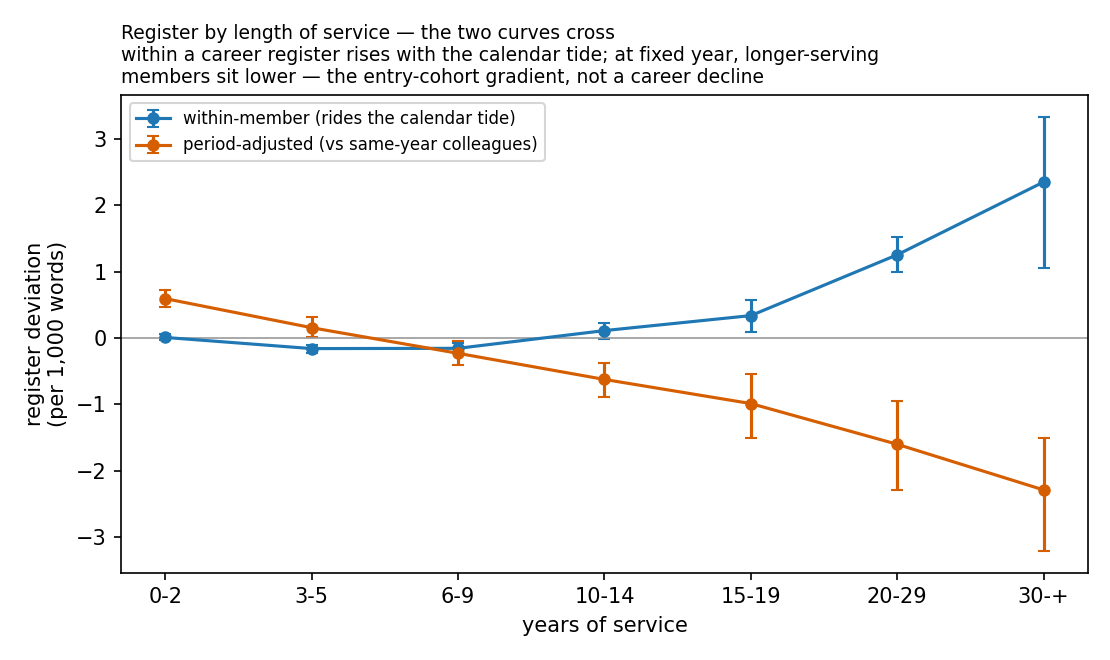
\includegraphics[width=0.85\linewidth]{tenure_profile.png}
\caption{Register by length of service, two readings, each curve labelled in the panel. The within-member curve (blue) --- each legislator\textquotesingle s rate minus their own career mean --- rises with tenure, because within a career years served and calendar year are one clock (its slope reproduces the +0.51 within-member drift). The period-adjusted curve (orange) --- rate minus its chamber \(\times\) year mean --- falls with tenure, but that fall is the entry-cohort gradient (longer tenure at a fixed year = earlier cohort), not a within-career decline. Left-censored members dropped; error bars member-cluster bootstrap 95\% intervals.}
\label{fig:tenure}
\end{figure}

\textbf{Splitting that career drift by birth cohort, every cohort rides the tide up --- but not in every chamber.}~(\cref{fig:lifedrift}) Running the same within-member estimator separately within each birth cohort (so the cohort numbers decompose the pooled +0.57 rather than averaging noisy per-member slopes) gives a positive-or-flat lifetime drift for every cohort, a shallow hump peaking at the 1950s-born (+0.88) and tapering at both thin tails. So the gain a member makes over their career barely depends on when they were born --- nearly everyone absorbs the drift they serve through. Interesting for the caveat it forces: the drift is \textbf{positive within members in only 10 of the 22 chambers}, carried by the two largest (UK +1.9, US House +0.5) while most of the smaller chambers --- the Canadian provinces especially --- run negative, so "sitting members convert" is a pooled, large-chamber statement rather than a universal one. And it is calendar drift ridden inside a career, not proven personal conversion: a member serving 2006--2026 gains register partly because the register rose under everyone. †\footnote{\texttt{python\ lifetime\_\allowbreak{}drift\_\allowbreak{}by\_\allowbreak{}cohort.\allowbreak{}py}. The committed within-member estimator (\texttt{cohort\_\allowbreak{}vs\_\allowbreak{}period.\allowbreak{}within\_\allowbreak{}member}) restricted to each birth cohort\textquotesingle s members --- demean rate and spoken year within each member, word-weighted, pool, per decade --- so each cohort is a decomposition of the pooled slope, not a mean of per-member slopes. Members need \(\geq\)3 years at \(\geq\)2,000 words; member-bootstrap CIs, seed 29. Pooled +0.57 reproduces the committed within-member figure; positive within-member drift in 10 of 22 chambers (per-chamber tally in the script output).}

\begin{figure}[htbp]
\centering
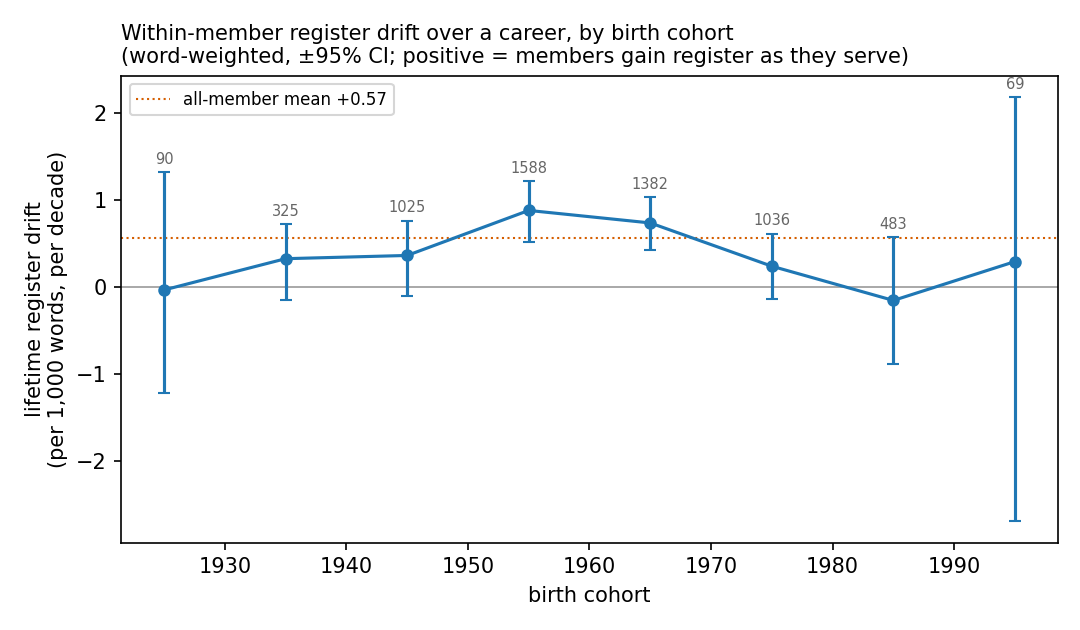
\includegraphics[width=0.85\linewidth]{lifetime_drift_by_cohort.png}
\caption{Within-member (lifetime) register drift by birth cohort --- the paper\textquotesingle s within-member estimator run inside each 10-year cohort, word-weighted, \(\pm\)95\% member-bootstrap CI. Positive means members gain register as they serve. The drift is positive or flat for every cohort and barely depends on birth year; the dotted line is the all-member pooled mean (+0.57, reproducing the committed within-member figure). Not uniform across legislatures --- see text. (\texttt{python\ lifetime\_\allowbreak{}drift\_\allowbreak{}by\_\allowbreak{}cohort.\allowbreak{}py}. The committed within-member estimator (\texttt{cohort\_\allowbreak{}vs\_\allowbreak{}period.\allowbreak{}within\_\allowbreak{}member}) restricted to each birth cohort\textquotesingle s members --- demean rate and spoken year within each member, word-weighted, pool, per decade --- so each cohort is a decomposition of the pooled slope, not a mean of per-member slopes. Members need \(\geq\)3 years at \(\geq\)2,000 words; member-bootstrap CIs, seed 29. Pooled +0.57 reproduces the committed within-member figure; positive within-member drift in 10 of 22 chambers (per-chamber tally in the script output).)}
\label{fig:lifedrift}
\end{figure}

\textbf{What the gradient is not.} It is not ministerial office: in the chambers whose record marks rank it \emph{strengthens} when office years are removed, and office-holders use less of the register than backbenchers, not more (Appendix~\ref{sec:cohort-ministerial}). It holds within year and province at \textbf{+1.05 per 1,000 per decade} (t \(\approx\) 8.5, clustered on member), unmoved by occupation and education controls --- which \emph{strengthen} it rather than explain it away (\cref{sec:four-predictors}). And the mechanism behind any component stays open: three exposure tests failed to isolate one (Appendix~\ref{app:null}). †\footnote{\texttt{python\ formation\_\allowbreak{}window.\allowbreak{}py}, clustered on member (CR1): birth-decade coefficient +1.05 per 1,000 words per decade, t = +8.46 unadjusted and +9.23 with occupation and education controls. The controls \emph{strengthen} the cohort term (coefficient +1.05 \(\rightarrow\) +1.14), which is why they are reported as running the wrong way for a selection story. The member-year HC1 errors the script also prints inflate the t to +17.7 --- a third instance of the unclustered-inference pattern flagged in Appendix~\ref{app:null}, though here, with 888 member clusters, the conclusion is unmoved.}

\textbf{What the family supports, and what it cannot.} No view settles the age-versus-cohort split; the identification wall stands, and the paper does not pretend otherwise. But the views are consistent and mutually reinforcing: a juniority gradient that is steady across legislatures at the individual level (space), exists before the models (pre-drift), bends upward exactly as drift-formed cohorts arrive (the one identification-free time statement), and is one members ride up within their own careers rather than only through replacement. The single citable figure --- stated as the identified cohort\(-\)age combination, not a pure cohort effect --- is birth-decade \textbf{+0.92 (t = 12.5)} in the member-year panel with year fixed effects, carried in \cref{sec:four-predictors} beside the other member-level predictors.

\subsection{The class coding: the same shape at coarser grain --- education}\label{sec:class}

The categorical schema that first revealed the gradient is kept here in abbreviated form: it shows the same shape as the altitude measure at coarser grain, and in the joint model below the measure absorbs it. Class predicts the register as a joint block --- an inverted U, peaking one rung below the top --- and the apparent education gradient does not survive its controls. On the eight provinces, class, education and prominence appeared to predict the register at t = 3--4; clustering by member and replication then removed every individual certainty. The joint tests say otherwise:

\textbf{Clustering the standard errors by member} (the study\textquotesingle s third encounter
with unclustered inference flattering a result) leaves the provincial point
estimates untouched and doubles to triples their errors: class II falls from
t = 3.40 to 1.48, IVab from 3.51 to 1.49, VIIab from \(-4.04\) to \(-1.84\), the
education ladder from 2.96 to 0.78. Member-years are not independent draws,
and treating them as such had manufactured the significance.

\textbf{Replication on the tier-1 panel} (US House, US Senate, UK Commons, federal
Canada, Dáil Éireann --- 18,178 member-years, 2,742 members, clustered) finds
the same qualitative shape at smaller magnitude --- II +0.24 and IVab +0.28
above class I, VIIab \(-0.51\) below --- with nothing individually significant
except class III, which is significant with the OPPOSITE sign to its
provincial estimate, i.e. noise behaving like noise.

The final specification --- one observation per legislator at equal weight,
register z-scored within each legislature against its full member
population, HC1 errors, joint Wald beside every table
(the reasoning for each choice is recorded with the estimator\footnote{\texttt{member\_\allowbreak{}level\_\allowbreak{}estimation.\allowbreak{}py}; each choice\textquotesingle s reasoning is in its
  docstring.}) ---
settles the section:

\textbf{Class is an inverted U, peaking one rung below the top.} At member level
across 22 chambers (n = 4,896, joint Wald \textbf{p = 0.0000}), reading the raw
within-chamber means so that every class stands on its own rather than against
a baseline:

\begingroup\small
\begin{longtable}[]{@{}lll@{}}
\caption{Register by EGP social class (member-level means).}\label{tab:egp}\\
\toprule\noalign{}
EGP class & mean z & n \\
\midrule\noalign{}
\endfirsthead
\toprule\noalign{}
EGP class & mean z & n \\
\midrule\noalign{}
\endhead
\bottomrule\noalign{}
\endlastfoot
I higher service & \(-0.088\) & 1,767 \\
\textbf{II lower service} & \textbf{+0.020} & 2,049 \\
III routine non-manual & +0.036 & 147 \\
IVab petty bourgeoisie & \(-0.092\) & 425 \\
V/VI skilled manual & \(-0.200\) & 222 \\
VIIab semi- and unskilled & \(-0.403\) & 109 \\
IVc farmers & \(-0.439\) & 177 \\
\end{longtable}
\endgroup

Class II sits above class I, and everything below the service classes falls
away sharply. Against class I the contrasts are II \textbf{+0.073 (t = 2.49)}, IVc
\(-0.260\) (t = \(-3.82\)), V/VI \(-0.161\) (t = \(-2.63\)), VIIab \(-0.252\) (t = \(-2.99\)); under
chamber fixed effects on raw rates the crossover is larger still, +0.650
(t = 5.17). III is nominally the highest cell but rests on 147 members and is
not distinguishable from II.

\textbf{The shape holds in every period, and does not migrate.} A chase-and-flight
cycle predicts that the originating tier abandons the form first, so the peak
should slide downward across eras. It does not. In six equal five-year bins
anchored at the data\textquotesingle s end --- 1997--2001 through 2022--2026, so the machine era
arrives whole as the final bin and the two years cut are the earliest, not
the newest --- class II sits above class I in every bin (\cref{fig:class-era}), the machine-era bin
included (II +0.04 against I \(-0.04\)), and the pooled manual-and-farm tail
stays below the pack throughout, visibly from 1997 once the thin early cells
are drawn rather than filtered. Two slow relative movements are visible
inside the stable shape, and they run in the same direction: the II-over-I
gap is narrowest in the machine-era bin (+0.08, against a series high of
+0.23), and V/VI drifts from \(-0.28\) toward zero across the series. That is
compression --- the lower tiers closing on the peak --- which is the chase
direction, not the flight direction, and it is neither significant (the gap
trend is \(-0.022\) per bin, t \(-1.67\)) nor aggregation-robust: weighting
member-years instead of members, the machine-era gap holds at +0.121
{[}+0.037, +0.202{]} and the trend flattens (\(-0.006\) per bin, t \(-0.4\)), so the
compression reading is the member-level view\textquotesingle s and is held lightly. The
peak itself never moves --- under either aggregation.†\footnote{\texttt{python\ build\_\allowbreak{}class\_\allowbreak{}by\_\allowbreak{}era.\allowbreak{}py} --- the committed generator:
  member-year panel rates z-scored against all member-years
  of their chamber \(\times\) half-decade, word-weighted to one value per member
  per bin, cells over the 5,391 class-coded members with any 1997+ speech;
  writes \texttt{class\_by\_era\_all.csv} (every cell) and the complete-bin paper
  files --- then \texttt{python\ plot\_\allowbreak{}class\_\allowbreak{}by\_\allowbreak{}era\_\allowbreak{}panels.\allowbreak{}py}. A member-\textbf{year}
  aggregation of the same data was checked directly
  (\texttt{peak\_decomposition.py}): the peak is II or III in every bin under
  member-level and member-year weighting alike --- class I is never the
  peak --- so the shape claim is aggregation-proof; the two weightings
  disagree only about how much the machine-era gap narrows, and that
  disagreement is reported above.}

\textbf{And the stable profile hides a renewal engine.} Decomposing each
class\textquotesingle s movement across the six bins into continuing members against
composition, \textbf{sitting members drift down relative to their chamber-and-
period peers in every transition} (the within term is negative in all ten
class-transitions, CIs excluding zero; class II stayers \(-0.75\) summed
across the series) \textbf{while entrants arrive above the stayers}, almost
exactly offsetting --- the register\textquotesingle s class profile is renewed by entry, not
maintained by incumbents. What II-over-I compression exists is a
within-member movement (\(-0.18\) {[}\(-0.32\), \(-0.03\){]}); its composition term is
indistinguishable from zero.\footnote{\texttt{python\ build\_\allowbreak{}member\_\allowbreak{}cache\_\allowbreak{}panel.\allowbreak{}py} (the panel-wide member \(\times\)
  word \(\times\) year cache, validated cell-for-cell against the committed
  member-year panel) then \texttt{python\ peak\_\allowbreak{}decomposition.\allowbreak{}py} --- both gap
  series with member-bootstrap CIs and the Firebaugh within/composition
  split, seed 7.}

\begin{figure}[htbp]
\centering
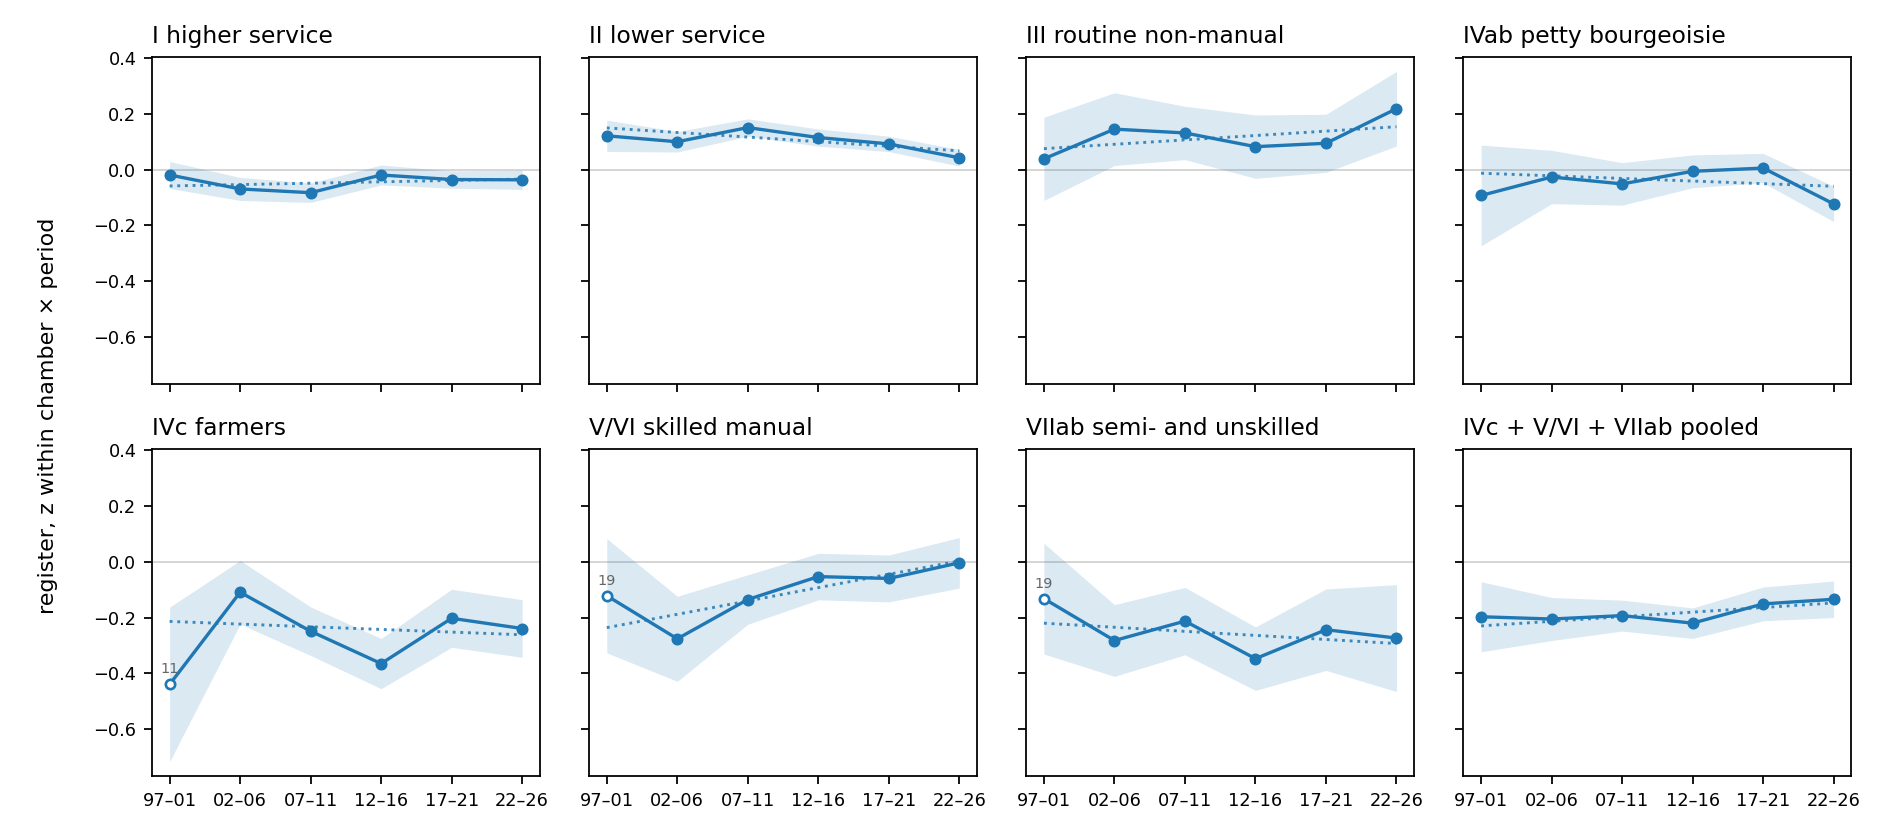
\includegraphics[width=0.85\linewidth]{class_by_era_panels.png}
\caption{The class profile of the register, 1997--2026, one panel per class plus
the pooled tail, in six equal five-year bins whose last is the machine era
(2022--26): member-level
means over 22 chambers, z-scored within chamber \(\times\) period, so the overall
era rise is removed and each panel reads as that class\textquotesingle s position against
its chamber-and-period average --- a rising panel is a class gaining relative
to its peers, not the register rising absolutely. Every cell with any
members is drawn; open markers carry fewer than 25 members (count
annotated). Error bars are \(\pm\)1 se; the dotted line is each panel\textquotesingle s
member-weighted linear trend. Class II holds above class I in every
bin; farmers and VIIab hold the floor; III --- thin at 26--85 members --- stays
elevated and tilts higher; V/VI climbs slowly toward zero, the one tail
series that moves; and the pooled tail (last panel) sits below the pack in
every bin.}
\label{fig:class-era}
\end{figure}

The era test cannot say who originated the form. Class I is never at the top,
not even in 1997--2001 --- but class coding only becomes substantial around 2005,
and \cref{sec:register-shift} dates the register\textquotesingle s turn to 1994--96. We are looking at a cycle
already in progress, with the crossover established before the first frame. The
study that would discriminate is class-coded Commons speech from 1985--1996,
where the deep archive reaches and occupations are recoverable (Appendix~\ref{app:future}).

\textbf{Who the peak actually is.} The classes are coded from members\textquotesingle{} own prior
occupations, so the peak has a concrete membership: class II is teachers (about
300 of them once the variants are pooled), journalists (73), social workers
(47), nurses (63). Class I, below it, is lawyers (roughly 500 across the four
national vocabularies), physicians, accountants, dentists, professors. The
petty bourgeoisie --- businessmen, small proprietors, realtors, insurance and
stock brokers --- is not elevated at all. The register is heaviest among the
\textbf{salaried, credentialled semi-professions}: the teaching, caring and
communicating occupations, credentialled but not elite-credentialled, employed
but not propertied. That is a description of who speaks it, not a claim about
where it came from --- \cref{sec:register-shift} dates the shift to 1994--96, before anything measured
here could have produced it.

\textbf{The II-over-I crossover is established, by the test that needs no normalization at all.} Comparing class II to class I WITHIN each chamber --- each legislature its own control, cohort-adjusted, equal member weights --- the contrast is positive in 9 of 12 chambers, individually significant in each of the three with the power to detect it (UK +0.68, t = 2.48; US House +0.82, t = 2.10; Manitoba +2.26, t = 2.21), and the inverse-variance meta-analysis across chambers gives \textbf{+0.59 per 1,000, z = 3.50}. One regression variant (full-population z-scoring) reads \(+0.054\sigma\) at t = 1.57 --- a diluted positive, not a contrary result: same sign as every other view, within 1.2 se of its sibling regression, short of the threshold because that scaling down-weights exactly the large low-variance chambers where the contrast is largest. Under heterogeneous per-chamber effects, differently weighted estimators answer differently weighted questions; no specification at any point estimated the contrast negative. (The within-chamber meta was computed after the variants diverged; it corroborates rather than adjudicates.) Teachers, nurses and journalists out-use lawyers, physicians and professors, within their own chambers, on both sides of the Atlantic. The exact location of any peak remains a non-claim: if the form is in flight the peak should migrate, so peak location is dynamics, not structure.

\textbf{Education makes the same inverted U, and it is the same people.} Read as
levels rather than as a ladder (22 chambers, n = 4,820 --- every member with
an education level, a birth year and a register score; cohort controlled,
baseline bachelor), with the graduate rung split by recorded degree --- master\textquotesingle s versus
doctorate --- where any source names one (61\% of graduate codings; the rest
stay a "graduate, degree unrecorded" level rather than being guessed or
dropped):\footnote{\texttt{python\ edu\_\allowbreak{}split\_\allowbreak{}graduate.\allowbreak{}py} --- degree markers (PhD/DPhil/
  EdD/ScD/ThD versus MA/MSc/MS/MBA/MEd/MPA/MPP/MSW/MPhil/LLM/MDiv/STM)
  regex-matched in each member\textquotesingle s recorded evidence quotes, education
  field and styled name, honorary-degree sentences stripped first;
  doctorate wins where both appear. A JD is deliberately not a doctorate
  here --- law belongs to the professional level. The script also prints
  this table.}

\begingroup\small
\begin{longtable}[]{@{}llll@{}}
\caption{Register by education level, relative to a bachelor's degree.}\label{tab:education}\\
\toprule\noalign{}
level & mean z & n & vs bachelor \\
\midrule\noalign{}
\endfirsthead
\toprule\noalign{}
level & mean z & n & vs bachelor \\
\midrule\noalign{}
\endhead
\bottomrule\noalign{}
\endlastfoot
none & \(-0.256\) & 14 & \(-0.232\) (t = \(-1.27\)) \\
secondary & \(-0.289\) & 287 & \textbf{\(-0.157\) (t = \(-2.81\))} \\
college & \(-0.174\) & 478 & \textbf{\(-0.153\) (t = \(-3.25\))} \\
\textbf{bachelor} & \textbf{+0.048} & 1,517 & baseline \\
master & +0.037 & 659 & \(-0.029\) (t = \(-0.68\)) \\
doctorate & +0.010 & 194 & +0.043 (t = +0.65) \\
graduate, degree unrecorded & \(-0.032\) & 625 & +0.053 (t = +1.31) \\
\textbf{professional} & \(-0.134\) & 1,046 & \textbf{\(-0.081\) (t = \(-2.16\))} \\
\end{longtable}
\endgroup

The plateau at the top is three levels wide --- bachelor, master and
doctorate sit within \(0.05\sigma\) of one another, so the graduate null is not an
artifact of lumping two credentials --- and both arms fall away
significantly: secondary and college by \textasciitilde\(0.15\sigma\), and on the descending side
the \textbf{professional} degree --- law and medicine, the most elite credential in \cref{tab:education} --- at \(-0.081\) on 1,046 members. Read as a straight line, this
would pass for an ascending "academic ladder" --- but only by excluding the
professional degree as off the ladder, the one category that breaks
monotonicity. The block is jointly significant on its own (Wald p = 0.0002
as level dummies).

It is not, however, an independent channel. Put class and education in one
model and the education block goes to \textbf{p = 0.27} while class holds at
\textbf{\(p < 10^{-4}\)} --- because the two instruments name the same stratum. Teachers,
nurses and social workers hold bachelor\textquotesingle s and master\textquotesingle s degrees; lawyers and
physicians hold professional ones. "Class II, not class I" and "bachelor or
graduate, not professional" are two descriptions of one group, so whichever
enters the model first absorbs the other. Education\textquotesingle s shape is real and
independently measured; its apparent separate effect is not.

\subsection{Socioeconomic position as organisational altitude: the register peaks at the insulated middle, and free work sits lowest}\label{sec:occupation}

The register peaks at the insulated middle of the organisational hierarchy and sits lowest among occupations that stand outside it. Each legislator\textquotesingle s prior occupation, coded to O*NET, is scored on an organisational-\textbf{altitude} ladder --- bottom, middle, top --- plus \textbf{free work}, the off-ladder level categorical class schemas do not carry. The ordering \textbf{free \textless{} front-line \textless{} corporate} was preregistered before any occupational element was joined to the register, and found. The ancestry is Weeden and Grusky\textquotesingle s\cite{weeden2005} case for measuring class at the disaggregated occupation, and Kohn and Schooler\textquotesingle s\cite{kohn1983} occupational self-direction, where closeness of supervision explained class differences in psychology; what the measure adds is distance from the hierarchy, not only altitude within it. What follows is the U over those levels, the off-ladder level\textquotesingle s stability across three decades, and, in the joint model below, the absorption of the class label the measure refines.

\textbf{The measure follows the discovery.} The register\textquotesingle s
occupational shape was first seen through the class coding (\cref{sec:class}): an
inverted U, peak one rung below the top, with no mechanism attached. This
arm registered one, built the instrument to measure it, and ran --- the
registration carries every revision and amendment dated,\footnote{\texttt{plans/\allowbreak{}PREREG-\allowbreak{}occupational-\allowbreak{}accountability.\allowbreak{}md} is the
  registration; \texttt{METHODOLOGY.md} §6.1c is the method record; the member table
  is \texttt{prereg\_\allowbreak{}member\_\allowbreak{}table.\allowbreak{}json}.} and every
number below reproduces from a committed script on a single member table
(one join; n = 4,762 members with register and
instrument, 3,594 with every covariate).

\textbf{The instrument, in one paragraph.} Each legislator\textquotesingle s prior occupation,
double-blind coded to an O*NET-SOC code, joins 64 O*NET elements whose
assignment to four components was itself blind-derived by three independent
coding workflows over the full 295-element universe: \textbf{U} upward (advising
without the final say; discretion reverse-scored), \textbf{L} lateral (external
service), \textbf{D} downward (command), \textbf{N} undirected (organisational
account-giving and contact). From the components and from an independent
blind coding of hierarchy positions come the study\textquotesingle s registered structure ---
\textbf{four levels, built two semi-independent ways}: the \emph{theoretical ladder}
(free / bottom / middle / top composed from the components) and the \emph{folk
ladder} (the same four levels scored from the element signatures of coders
asked to concretize the everyday image of a corporate hierarchy, never told
the register or the hypothesis existed) --- plus
the \textbf{apex delta} (MIDDLE \(-\) TOP), registered in words as "insulated command
tracks more register than exposed command."

\textbf{The four-level U is the result, and its registration is a timeline.} The
middle-peak prediction --- free and the top low, the middle the peak --- was
stated in the session log an hour before the first fit; the folk ladder and
the apex delta entered the committed pre-registration twelve minutes before
it; the theoretical ladder\textquotesingle s explicit sign declarations were formalised in
the post-Stage-1 amendment. The exact record, to the minute, is in the
footnote.\footnote{The registration record, all times 2026-08-18 US-Pacific, from the
  session transcript and git. \textbf{12:04}, session log, before any fit or
  instrument freeze: "I would actually expect the highest reading to come
  with middle managers with workers below them" (Matthew). \textbf{12:41}: the
  four-level structure directed ("three levels of corporate and a free").
  \textbf{13:03}: the charged/uncharged horse race directed. \textbf{13:05}, commit
  \texttt{f10d502}: the folk ladder and the apex delta ("insulated command
  tracks more register than exposed command") committed to the prereg.
  \textbf{13:17}, \texttt{ad303ad}: Stage 1 run and unblinded. \textbf{13:36}, \texttt{53a02ff}:
  amendment adding the theoretical ladder and the explicit middle+/free\(-\)
  sign declarations, self-labelled as post-unblinding. \textbf{17:21},
  \texttt{ccba83d}: the ruling recording the U as the design intent. So the
  prediction precedes the data by 73 minutes in the log, and the formal
  document carries the apex delta pre-run; what is post-run is
  formalisation, not prediction. The meta-point is worth naming: under
  machine execution with pervasive logging, the timestamped record that
  pre-registration exists to create is produced continuously, and the
  spirit of the practice --- predictions verifiably preceding data --- is
  checkable to the minute without the formal document as the only witness.} Each
level entered alone (standardised; n = 4,762, full-covariate slopes at
n = 3,594):

\begingroup\small
\begin{longtable}[]{@{}lll@{}}
\caption{The occupational altitude ladder: register by level on both constructions (plotted in \cref{fig:altitude}).}\label{tab:altitude}\\
\toprule\noalign{}
level & theoretical ladder & folk ladder \\
\midrule\noalign{}
\endfirsthead
\toprule\noalign{}
level & theoretical ladder & folk ladder \\
\midrule\noalign{}
\endhead
\bottomrule\noalign{}
\endlastfoot
free & \(-0.060\) (t \(-4.2\)) & \(-0.066\) (t \(-4.7\)) \\
bottom & \(-0.021\) (t \(-1.5\)) & +0.010 (t +0.7) \\
\textbf{middle} & \textbf{+0.029 (t +2.0)} & \textbf{+0.028 (t +2.0)} \\
top & +0.010 (t +0.7) & +0.021 (t +1.5) \\
\end{longtable}
\endgroup

Middle peak, top below it, free at the floor, bottom indistinguishable from
zero --- the II-over-I crossover in occupational form, from two instruments
built by different processes, agreeing at the peak to the third decimal.
Both middles survive the full covariate set (+0.041 and +0.042, t 2.6
each); under covariates the shape sharpens (bottom mildly negative, top
close behind middle), and the middle-over-top gap\textquotesingle s powered test is the
delta. The registered \emph{continuous} form of the interior peak --- the altitude
quadratic --- found nothing (Appendix~\ref{app:null}18); the discrete levels and the
relative contrast carry the claim (\cref{fig:altitude}).

\begin{figure}[htbp]
\centering
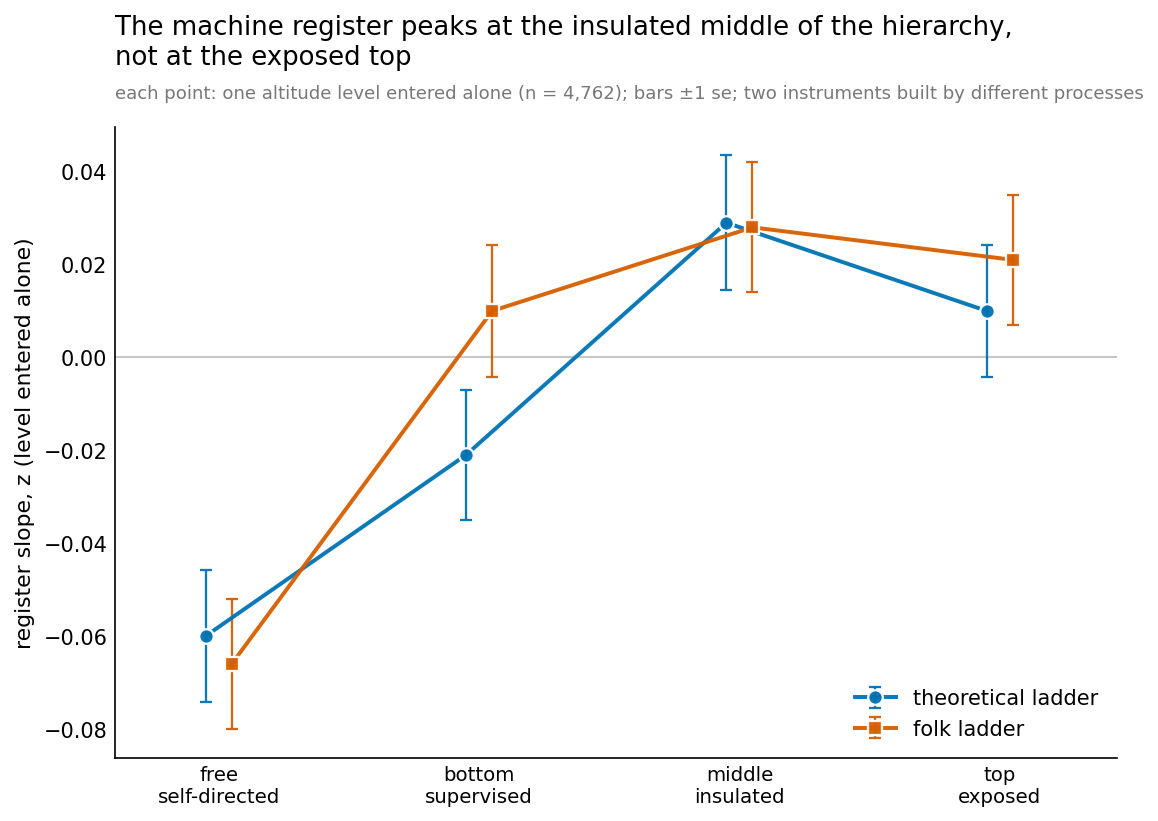
\includegraphics[width=0.85\linewidth]{altitude_u.png}
\caption{The occupational register profile. Each legislator\textquotesingle s prior occupation, coded to O*NET, is scored on a four-level altitude ladder (free / bottom / middle / top of an organisational hierarchy) two semi-independent ways --- the theoretical ladder and the folk ladder --- and both peak at the insulated middle, dipping at the exposed top. Points are each level\textquotesingle s base slope entered alone (standardised, n = 4,762); bars \(\pm\)1 se. The levels are individually noisy but jointly significant; the powered claim is the apex delta (middle \(-\) top), +0.049 (t 3.3), rising to +0.067 (t 3.9) under full covariates.}
\label{fig:altitude}
\end{figure}

\textbf{The delta is the study\textquotesingle s most covariate-robust occupational number.}
Registered in words and observed +0.049 (t 3.3) raw; \textbf{+0.067 (t 3.9)}
with cohort, class, education and prominence all present; right-signed and
nominally significant in 16 of 16 covariate specifications; it absorbs the
theoretical middle entirely when both enter. Dropped from the grand model
it costs as much adjusted \(R^{2}\) as the entire six-dummy class block (.0033 vs
.0038); education is spent once class and the delta are present (.0004).
Its group form --- members split by relative inwardness, insulated against
exposed --- puts the insulated cell above the rest (t 2.1 on the gap), with
one leg farmer-driven and reported as such: the 199 members the instrument
reads as agricultural managers sit in the exposed cell and drag it, exactly
the headwind the registration\textquotesingle s prediction 5 named in advance.

\textbf{Era-resolved, the instrument\textquotesingle s carrying level is stable.} The joint
model\textquotesingle s surviving occupational block is the folk ladder, and its standing
term is the free level; asked era by era --- each level\textquotesingle s slope entered
alone, \cref{fig:altitude}\textquotesingle s own estimand, on the same member-bin values and
six equal bins as \cref{sec:class}\textquotesingle s class-era panels --- free professionals sit below their
chamber-and-period peers in every half-decade (\(-0.07\) to \(-0.11\) per sd,
individually significant in all six bins), with no trend into the machine
era, while bottom, middle and top stay small and flat (formally: no
level\textquotesingle s era trend approaches significance --- free z +1.2, middle \(-1.0\),
top \(-0.8\), apex delta \(-0.2\)). Like the class shape, the occupational shape
was in place decades before the machines.~(\cref{fig:ladder-era})\footnote{\texttt{python\ build\_\allowbreak{}ladder\_\allowbreak{}by\_\allowbreak{}era.\allowbreak{}py}, then
  \texttt{python\ plot\_\allowbreak{}ladder\_\allowbreak{}by\_\allowbreak{}era\_\allowbreak{}panels.\allowbreak{}py}.}

\begin{figure}[htbp]
\centering
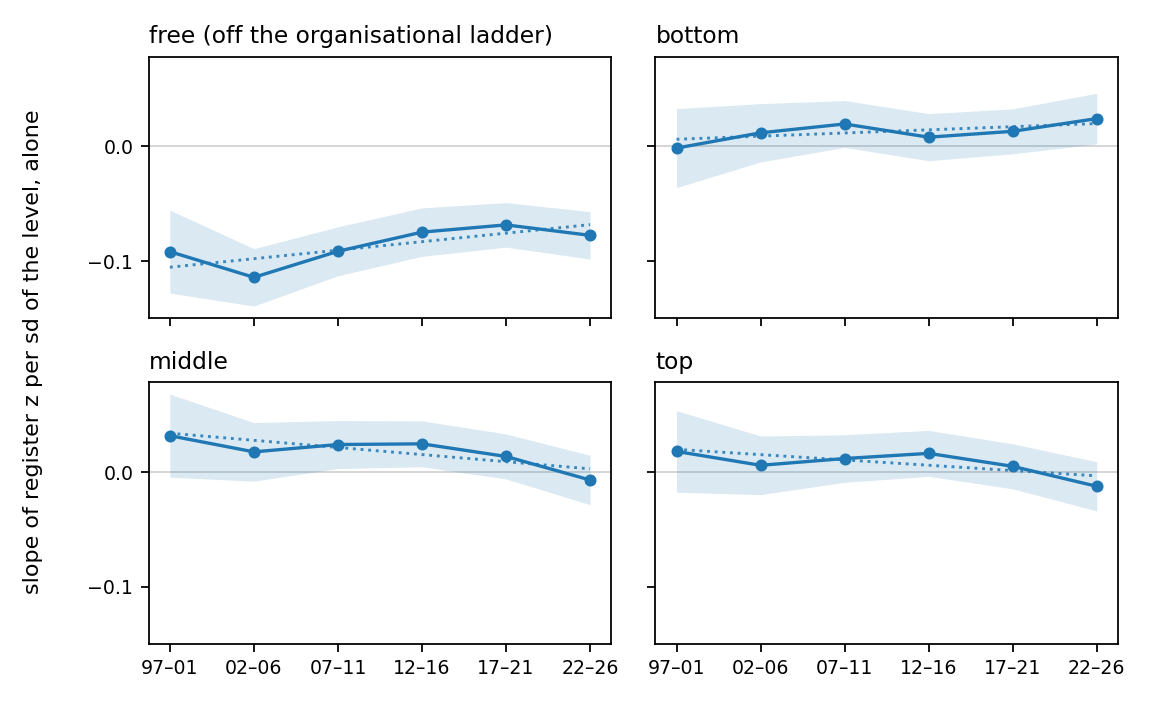
\includegraphics[width=0.85\linewidth]{ladder_by_era_panels.png}
\caption{The coded altitude ladder across eras: each level\textquotesingle s slope entered alone
(per sd, HC1 errors), on the same member-bin values and six equal five-year
bins as the class panels; \(\pm\)1 se bands, dotted member-weighted linear
trends. The free level --- professionals off the organisational ladder ---
carries the instrument in every half-decade; the three on-ladder levels
stay small and flat.}
\label{fig:ladder-era}
\end{figure}

\textbf{And it holds chamber by chamber, by the test that needs no
normalization.} The class arm\textquotesingle s crossover claim rests on a within-chamber
meta-analysis; the measure gets the same test. Within each chamber --- each
legislature its own control --- the member-level slope of the register on the
free level is \textbf{negative in 21 of 22 chambers} (individually significant
in Queensland and Scotland), and the inverse-variance meta across chambers
is \textbf{\(-0.070\) per sd, z = \(-5.0\)}; the apex delta pools at \textbf{+0.059, z =
+4.2}. Split by chamber group the replication is a sweep --- negative in every
group: the nine 2026 additions (meta z \(-4.1\)), the eight Canadian provinces
(z \(-2.5\)), and the five tier-1 national chambers (z \(-2.2\)).\footnote{\texttt{python\ ladder\_\allowbreak{}chamber\_\allowbreak{}meta.\allowbreak{}py} --- per-chamber OLS slope of
  member z on the folk free level (per sd within chamber, HC1),
  inverse-variance pooled; the apex-delta meta from the same cells.}

\textbf{Against the market-fitted measures.} The classical anchors join at
occupation level through the study\textquotesingle s existing SOC coding --- no new member
placement anywhere --- via the BLS crosswalk to ISCO-08 for Ganzeboom\textquotesingle s ISEI
and Treiman\textquotesingle s SIOPS prestige scale, OES national median wages, and O*NET\textquotesingle s
Job Zone and required-education categories.\footnote{\texttt{python\ build\_\allowbreak{}market\_\allowbreak{}join.\allowbreak{}py} then
  \texttt{python\ market\_\allowbreak{}convergence.\allowbreak{}py}; source files and fetch provenance in
  \texttt{market\_\allowbreak{}anchors/\allowbreak{}PROVENANCE.\allowbreak{}md}. Coverage: 351 of 401 study occupations
  carry level scores; ISEI misses 15\% of codes because the official
  crosswalk is 2010-SOC-vintage against the study\textquotesingle s 2018-based O*NET
  codes; SOC codes mapping to several ISCO-08 codes (63) take the mean
  of the mapped scores.} Convergently, the
ladder sits inside the socioeconomic family without being any member of
it: member-weighted Cramér\textquotesingle s V between the folk argmax level and each
anchor runs 0.31 (wage quartiles) to 0.47 (SIOPS quartiles). Discriminantly,
it is not the old ingredients recombined: regressing each level score on
occupational education and log wage leaves \(R^{2}\) at 0.32--0.45, so more than
half of every level\textquotesingle s variance lies off the education--earnings plane --- and
the free level is not self-employment in disguise (free-argmax members are
petty bourgeois or farmers at 6\%, against the panel\textquotesingle s 14\%). The extremes
are face-valid and occasionally sharper than the schemas: painters and
craft artists score free-high while actors and dancers --- performers, who
work under direction --- score free-low, a distinction no market category
draws. And in the joint model the asymmetry is complete: entered as
member-weighted quartile dummies beside the committed blocks, \textbf{ISEI and
wage collapse (block p = 0.31 and 0.35) while the folk ladder stands
(p = 0.017, its free level \(-0.089\), t \(-3.08\), with both anchors in)} ---
alone on the same 3,276 members all three are strong (folk \(p < 10^{-7}\), ISEI
\(p < 10^{-6}\), wage p = 0.003). The fitted scales are absorbed by the study\textquotesingle s
covariates; the blind measure is not absorbed by the fitted
scales.\footnote{\texttt{python\ market\_joint.py} --- the committed member-level spec
  (z within chamber, equal weight, HC1, block Walds) on the 3,276
  members carrying every block, with ISEI and log-wage entered as
  member-weighted quartile dummies, Q1 baseline.}

\textbf{The gradient nests inside class, which is what "the class U was
occupation all along" requires.} The delta\textquotesingle s slope within class II alone is
+0.076 (t 3.3) --- the class peak\textquotesingle s own interior carries the occupational
gradient --- and +0.066 (t 4.0) with class fixed effects. Prediction 1 (the
occupational block adds to EGP) confirmed in 16 of 16 paired
specifications.

\textbf{The horse race and the pattern.} The uncharged (coded) instrument wins
the registered AIC comparison narrowly (\(-205.0\) vs \(-198.6\)); encompassing
tests are significant in both directions --- neither instrument subsumes the
other. The registered four-sign component pattern (U+ L\(-\) D+ N+) holds in
25\% of pattern-eligible lattice specifications, permutation p = 0.087
across 2,000 within-chamber shuffles --- suggestive, unconfirmed. Under the
covariate lattice, L\textquotesingle s raw positivity dissolves (median +0.012,
direction-unstable): the external-service gradient was carrying class and
education correlation rather than surviving it, while U and N stay
right-signed in 100\% of specifications and D turns mildly positive
throughout.

\textbf{Era restriction} (2025--26 speech only, n = 1,000): cohort deflates to
its period-purged size (+0.138/sd, t 4.3 --- the career figure of +0.383 was
mostly period mixing), the class-II contrast doubles to +0.203 (t 3.0), and
the delta persists directionally at era power (+0.061, t 1.7; the career
effect predicts t \(\approx\) 2.0 at this n). In the spike window, class II is the
strongest social-position covariate; the insulation contrast holds its size
without independent confirmation.

One drafting generation of the registration expressed the peak claim as a
linear three-profile rank; that operationalization failed its own test and
the framing is retired --- Appendix~\ref{app:superseded}13 preserves its numbers, and the
registration\textquotesingle s post-run amendment records the oversight and the provenance
ruling. Failed registered predictions are in Appendix~\ref{app:null} (the altitude
quadratic, the autonomy asymmetry, nominal-vs-effective autonomy). Scale
for all of it: \cref{sec:limits}\textquotesingle s calibration bullet --- small effects by any benchmark,
reliably estimated, structurally replicated, floors rather than
ceilings.\footnote{\texttt{python\ prereg\_\allowbreak{}stage1.\allowbreak{}py}, \texttt{prereg\_stage2.py},
  \texttt{prereg\_\allowbreak{}synthesis\_\allowbreak{}check.\allowbreak{}py}, \texttt{prereg\_\allowbreak{}covariate\_\allowbreak{}strength.\allowbreak{}py},
  \texttt{prereg\_\allowbreak{}strength\_\allowbreak{}2526.\allowbreak{}py}; results snapshots
  \texttt{prereg\_\allowbreak{}stage1\_\allowbreak{}results.\allowbreak{}txt}, \texttt{prereg\_\allowbreak{}stage2\_\allowbreak{}results.\allowbreak{}txt}. The join and
  its drift guard: \texttt{prereg\_join.py} (\texttt{METHODOLOGY.md} §6.1b addendum for the
  two join facts). Instrument derivation artifacts:
  \texttt{element\_audit\_*.json}, \texttt{element\_levels.json},
  \texttt{instrument\_\allowbreak{}final\_\allowbreak{}cells.\allowbreak{}json}.}

\textbf{The coarsest cut is the strongest single correlate: the register is the
language of the office.} O*NET\textquotesingle s \emph{Indoors, Environmentally Controlled} ---
planted in the element pool as a deliberately atheoretical marker of office
work --- carries more register per standard deviation than any single
instrument component (+0.101, t +7.4); \emph{Spend Time Sitting}, the other
planted marker, is null (t +0.4). This is the occupational finding at its
coarsest resolution, a restatement rather than a rival: office work carries
the register wholesale, and the structure this section measures is the shape
inside the office --- the insulated middle over the exposed top, both of them
office rungs, and free work lowest. In the joint model the office cut adds
little that the existing covariates do not already carry (+0.039 per sd,
t +1.9, \(\Delta\text{adj}R^{2}\) +0.0007), and the apex delta stays the strongest occupational
term in that model (t +2.4, \(\Delta\text{adj}R^{2}\) +0.0011) --- birth decade remains the
overwhelming axis (t +24.5, carrying 0.144 of the model\textquotesingle s 0.165).\footnote{\texttt{python\ prereg\_\allowbreak{}negative\_\allowbreak{}controls.\allowbreak{}py}; n = 4,762, estimator
  parity-guarded against stage 1 (reproduces MIDDLE +0.028, t 2.0).
  Entered jointly with Indoors, the apex delta reads +0.033 (t +2.2) and
  free \(-0.062\) (t \(-4.4\)). The pre-registration had planted these two
  elements as negative controls with an office-job interpretation rule;
  the adjudication (2026-08-24, logged in the prereg) rejects that rule\textquotesingle s
  implication --- office language is the finding restated, not a control on
  it --- and the result is reported here as description. Joint-model numbers:
  \texttt{python\ prereg\_\allowbreak{}indoors\_\allowbreak{}joint.\allowbreak{}py} (n = 3,594, the covariate panel; the
  grand model mirrors \texttt{prereg\_\allowbreak{}covariate\_\allowbreak{}strength.\allowbreak{}py}).}

\subsection{All four predictors at once}\label{sec:four-predictors}

Every member-level predictor in one regression --- every category of every
block, none folded into a baseline for being small or dropped from the table
for being null. Four blocks fit on the full panel (n = 4,056 complete cases
across 22 chambers): cohort, all seven EGP classes, all education levels,
and prominence as article-length quintiles --- the bins, not a line, because
Appendix~\ref{sec:prominence-buckets} shows the shape is not linear. The occupational blocks then
enter on the members with occupational-score coverage (n = 3,631): \cref{sec:occupation}\textquotesingle s
two altitude ladders, each with all four levels per sd, plus Indoors. Each
block is also fitted alone on the same sample, so attenuation is read
against its own baseline; t in parentheses; the last column converts
jointly-significant effects into years of cohort: †\footnote{\texttt{python\ joint\_\allowbreak{}predictors.\allowbreak{}py}. Canonical member-level spec --- one
  observation per legislator, equal weight, register z-scored within chamber
  against the chamber\textquotesingle s full member population, HC1 errors, block Wald over
  every block\textquotesingle s term vector (1-df blocks included, where it is the t test).
  "Alone" is the block fitted by itself on the same sample (no other
  covariates), so the columns read raw association \(\rightarrow\) survives the other
  blocks \(\rightarrow\) survives the occupational content too. Education enters as
  level dummies with bachelor baseline --- the education table\textquotesingle s coding,
  graduate rung split by recorded degree (\texttt{edu\_split\_graduate.py}) ---
  and every category present enters as a dummy, education\textquotesingle s "none" and
  every EGP class included. Prominence quintiles are cut on each estimation sample\textquotesingle s log article
  lengths (Q1 baseline). The occupational blocks are \cref{sec:occupation}\textquotesingle s two altitude
  ladders --- directional and coded, all four levels each, standardised per
  sd on the occ panel --- plus Indoors. The prereg\textquotesingle s apex delta is
  identically lvl MIDDLE \(-\) lvl TOP (verified to machine precision), so the
  coded-ladder block subsumes it and must not enter beside it; the
  prereg\textquotesingle s never-together rule for the twin ladders is deliberately
  relaxed here, and the price is visible in the widened joint SEs on the
  twinned levels.}

\begingroup\small
\begin{longtable}[]{@{}p{0.255\linewidth}rp{0.135\linewidth}p{0.135\linewidth}p{0.135\linewidth}l@{}}
\caption{Every member-level predictor in one model: each block alone, the joint fit of cohort, all EGP classes, all education levels and prominence quintiles (n = 4{,}056), and the occupational blocks — both altitude ladders and Indoors — added (n = 3{,}631); t in parentheses; the last column converts jointly significant effects into years of cohort.}\label{tab:four-predictors}\\
\toprule\noalign{}
term & n & alone & joint & + occ. blocks & \(\approx\) yrs \\
\midrule\noalign{}
\endfirsthead
\toprule\noalign{}
term & n & alone & joint & + occ. blocks & \(\approx\) yrs \\
\midrule\noalign{}
\endhead
\bottomrule\noalign{}
\endlastfoot
\textbf{cohort} (per decade) & 4,056 & +0.276 (27.7) & \textbf{+0.272 (26.9)} & +0.266 (24.5) & \emph{the scale} \\
--- block Wald (1 df) & & \(p < 10^{-70}\) & \(p < 10^{-67}\) & \(p < 10^{-59}\) & \\
\textbf{class} (baseline I, \emph{n} 1,660) & & & & & \\
\(\cdot\) II lower service & 1,691 & +0.122 (3.63) & \textbf{+0.084 (2.44)} & +0.018 (0.41) & +3 \\
\(\cdot\) III routine non-manual & 116 & +0.084 (0.95) & +0.036 (0.42) & +0.024 (0.22) & --- \\
\(\cdot\) IVab petty bourgeoisie & 280 & +0.005 (0.08) & +0.002 (0.03) & +0.009 (0.12) & --- \\
\(\cdot\) IVc farmers & 109 & \(-0.339\) (\(-3.48\)) & \textbf{\(-0.201\) (\(-2.10\))} & \(-0.089\) (\(-0.75\)) & \(-7\) \\
\(\cdot\) V/VI skilled manual & 130 & \(-0.229\) (\(-2.79\)) & \textbf{\(-0.235\) (\(-3.02\))} & \(-0.204\) (\(-1.90\)) & \(-9\) \\
\(\cdot\) VIIab non-skilled manual & 70 & \(-0.384\) (\(-3.70\)) & \textbf{\(-0.286\) (\(-2.60\))} & \(-0.037\) (\(-0.23\)) & \(-11\) \\
--- block Wald (6 df) & & \(p < 10^{-4}\) & \textbf{\(p < 10^{-4}\)} & \textbf{p = 0.56} & \\
\textbf{education} (baseline bachelor, \emph{n} 1,190) & & & & & \\
\(\cdot\) none & 14 & \(-0.301\) (\(-1.70\)) & \(-0.161\) (\(-0.95\)) & \(-0.103\) (\(-0.53\)) & --- \\
\(\cdot\) secondary & 231 & \(-0.318\) (\(-4.61\)) & \(-0.049\) (\(-0.78\)) & \(-0.047\) (\(-0.70\)) & --- \\
\(\cdot\) college & 367 & \(-0.207\) (\(-3.67\)) & \(-0.062\) (\(-1.16\)) & \(-0.088\) (\(-1.52\)) & --- \\
\(\cdot\) master & 552 & \(-0.042\) (\(-0.85\)) & \(-0.066\) (\(-1.42\)) & \(-0.043\) (\(-0.87\)) & --- \\
\(\cdot\) doctorate & 173 & \(-0.054\) (\(-0.65\)) & +0.017 (0.24) & \(-0.016\) (\(-0.20\)) & --- \\
\(\cdot\) graduate, unrecorded & 541 & \(-0.097\) (\(-1.93\)) & +0.015 (0.32) & +0.008 (0.17) & --- \\
\(\cdot\) professional & 988 & \(-0.174\) (\(-4.11\)) & \(-0.088\) (\(-1.98\)) & \(-0.094\) (\(-1.92\)) & --- \\
--- block Wald (7 df) & & \(p < 10^{-4}\) & \textbf{p = 0.27} & p = 0.45 & \\
\textbf{prominence} (article-length quintile, baseline Q1) & & & & & \\
\(\cdot\) Q2 & 812 & \(-0.018\) (\(-0.37\)) & \(-0.069\) (\(-1.62\)) & \(-0.059\) (\(-1.31\)) & --- \\
\(\cdot\) Q3 & 812 & +0.228 (4.68) & \textbf{+0.163 (3.70)} & +0.170 (3.62) & +6 \\
\(\cdot\) Q4 & 812 & +0.210 (4.39) & \textbf{+0.146 (3.24)} & +0.184 (3.82) & +5 \\
\(\cdot\) Q5 & 812 & +0.131 (2.77) & \textbf{+0.145 (3.22)} & +0.164 (3.36) & +5 \\
--- block Wald (4 df) & & \(p < 10^{-4}\) & \textbf{\(p < 10^{-4}\)} & \textbf{\(p < 10^{-4}\)} & \\
\textbf{theoretical ladder} (per sd, n 3,631) & & & & & \\
\(\cdot\) free & & \(-0.243\) (\(-4.80\)) & --- & \(-0.123\) (\(-1.21\)) & --- \\
\(\cdot\) bottom & & +0.084 (2.18) & --- & +0.082 (0.97) & --- \\
\(\cdot\) middle & & \(-0.136\) (\(-2.64\)) & --- & \(-0.166\) (\(-1.53\)) & --- \\
\(\cdot\) top & & +0.008 (0.21) & --- & +0.130 (2.09) & +5/sd \\
--- block Wald (4 df) & & \(p < 10^{-4}\) & --- & \textbf{p = 0.28} & \\
\textbf{folk ladder} (per sd, n 3,631) & & & & & \\
\(\cdot\) FREE & & \(-0.109\) (\(-4.70\)) & --- & \textbf{\(-0.090\) (\(-3.07\))} & \(-3\)/sd \\
\(\cdot\) BOTTOM & & +0.115 (3.21) & --- & \(-0.039\) (\(-0.61\)) & --- \\
\(\cdot\) MIDDLE & & \(-0.156\) (\(-1.35\)) & --- & +0.151 (0.72) & --- \\
\(\cdot\) TOP & & +0.356 (2.72) & --- & \(-0.164\) (\(-0.75\)) & --- \\
--- block Wald (4 df) & & \(p < 10^{-4}\) & --- & \textbf{p = 0.0008} & \\
\textbf{Indoors} (per sd, n 3,631) & & +0.091 (5.88) & --- & +0.033 (1.50) & --- \\
--- block Wald (1 df) & & \(p < 10^{-4}\) & --- & p = 0.13 & \\
\end{longtable}
\endgroup

Two robustness reads, both on the same 3,631 members. First, the

\begin{itemize}
\tightlist
\item
  occupational column\textquotesingle s changes come from the blocks, not the thinner
  sample: refit without them, the four blocks are essentially unchanged
  (cohort +0.266, II +0.084, class block p = 0.0004) --- except VIIab, which
  thins to 53 members and \(-0.183\) (t \(-1.43\)) before the blocks ever enter.
  Second, no block\textquotesingle s fate hangs on which ladder twin entered --- the fit is
  simultaneous, not sequential, and the leave-one-out variants confirm it:
  with only the theoretical ladder present, class is p = 0.62 (ladder
  p = 0.037, Indoors +0.056, t 2.77); with only the folk ladder, class is
  p = 0.54 (ladder \(p < 10^{-4}\), Indoors +0.047, t 2.30). Either ladder alone
  retires class; Indoors stays marginally alive beside either single ladder
  and is absorbed only by the pair; the folk ladder is the stronger carrier
  and takes the credit when both enter.
\end{itemize}

\textbf{Why the largest coefficients carry the least variance.} A term\textquotesingle s
variance share is per-member effect\({}^{2}\) \(\times\) member share. VIIab moves each of
its members more than ten cohort-years --- but 70 members are 1.7\% of the panel, so
the term carries \textasciitilde0.25\% of variance alone; class II\textquotesingle s far smaller +0.122 on
42\% of members carries more (\textasciitilde0.36\%), and cohort\textquotesingle s dominance comes from a
modest slope applied to everyone across a two-decade spread. Coefficients
answer "how much for whom"; variance shares answer "how much of the panel"
--- \cref{tab:four-predictors}\textquotesingle s n and years columns show the first, the explanatory-power
accounting below the second, and neither substitutes for the other.

\textbf{They do not deserve equal billing, and the full model says which is
which.} Cohort is untouched by anything and an order of magnitude better
resolved than the rest. Prominence, entered as the bins E.3 says it is,
survives everything at \(p < 10^{-4}\) in every column --- the hump sits inside the
joint model: flat through Q2, +0.16 to \(+0.19\sigma\) across Q3--Q5 with the top
quintile easing off the Q4 peak (entered as a line instead, the block
prints +0.020 per log-unit, t 2.05, and the shape disappears --- the line was
the wrong form, not the predictor). Class shows a wider floor than the
headline contrast --- all three manual-and-rural categories sit significantly
below the service classes jointly (V/VI \(-0.235\), VIIab \(-0.286\), IVc \(-0.201\)) ---
and survives cohort, education and prominence, but not its own finer
measurement: beside the altitude ladders the class block falls to p = 0.56,
and the leave-one-out fits show either ladder alone does it (p = 0.62 and
p = 0.54), because the EGP label is a coarse coding of the occupational
content the ladders measure directly. That is the joint model repeating
what destination-not-origin already said: the register tracks what the work
was, not what the label says. The same absorption runs inside the
occupational blocks themselves --- each is strong alone; the folk ladder is
the stronger carrier (p = 0.0008 with both in, its FREE level \(-0.090\) per
sd) and takes the credit from its theoretical near-twin, while Indoors
stays marginally alive beside either single ladder and is absorbed only by
the pair. That the folk ladder beats the theoretical one is itself a datum
for the introduction\textquotesingle s classification point: take the stereotype --- the
everyday picture of a corporate ladder --- have machine coders concretize it
blind, and the concretized folk category measures better than the
theory-built alternative. Education survives nothing, in any column --- and with the
graduate rung split, master\textquotesingle s and doctorate both sit at the bachelor
plateau, so the null is not a lumping artifact. What the full model keeps,
then, is cohort, the prominence bins, and one occupational ladder; what it
retires is the class label, education, and every occupational term the
ladders already encode.

Class needs the panel\textquotesingle s full power: restricted to the thirteen
pre-expansion chambers (n = 2,989), the II-over-I contrast falls to t = 1.26
and the block to p = 0.0074 --- cohort is collinear with both class and
education, and the smaller sample cannot separate them.

\textbf{Origin is null, and robustly so.} Parental class, 704 members, tested
under both the panel and member-level specifications: joint p = 0.53--0.59,
group means within \(0.1\sigma\) of each other. \textbf{The register tracks class
destination, not class origin} --- what a legislator did, not where they came
from --- which favours occupational practice over inherited-status accounts of
the gradient, stated as interpretation.

\textbf{The juniority gradient towers over all of it.} Birth decade is
\textbf{+0.92 (t = 12.5)} in the member-year panel with year fixed effects on
the current 22 chambers --- the citable figure, since career-level
specifications absorb era of service into the term --- read throughout as
the identified cohort\(-\)age combination (\cref{sec:generational}: its level is an age-or-career
clock under the Senate bound; its post-1985 bend is cohort) --- and
survives every covariate this study has measured, in three countries and 22
chambers. For scale: the whole class gradient --- II down to VIIab, jointly ---
spans \textasciitilde\(0.37\sigma\); cohort covers that in about fourteen years of birth date.

\textbf{Together they explain about a sixth of the variance.} The grand member-level model --- cohort, class, education, prominence, with \cref{sec:occupation}\textquotesingle s occupational ladder and office cut added --- reaches adjusted \(R^{2}\) \(\approx\) 0.16, and 0.14 of it is cohort alone; no other block contributes more than a few thousandths.\footnote{\texttt{python\ prereg\_\allowbreak{}covariate\_\allowbreak{}strength.\allowbreak{}py} and \texttt{python\ prereg\_\allowbreak{}indoors\_\allowbreak{}joint.\allowbreak{}py} (n = 3,594, the full-covariate member panel):
  grand adjusted \(R^{2}\) 0.1639 without and 0.1646 with the office cut; \(\text{adj}R^{2}\)
  lost if dropped --- birth decade 0.1444, apex delta 0.0011, Indoors
  0.0007, EGP 0.0006, prominence 0.0005, education 0.0003, dir middle
  \(-0.0001\) (the one block the model fits marginally better without).} So this is not a discovered instrument for identifying machine text by its company, or for reading a person\textquotesingle s history off their vocabulary, and the study should not be cited as one. What it is, is evidence that such structure exists: one borrowed 407-word ruler --- built from a different corpus for a different purpose --- carries a juniority gradient across forty years and five legislatures, an occupational shape built twice by blind processes, and a post-training signature, through a probe thin enough that five-sixths of member-level variation never enters it. The full register, and the web of relationships it participates in, has gone untracked; it is the kind of object machine intelligence turns searchable, which is why the register itself is queued as a search target rather than a fixed list (Appendix~\ref{app:future} items 33--34), and why the Limits read the small shares as floors of one thin probe rather than ceilings of the phenomenon.

\subsection{Chase and flight: an exploratory interpretation of the social gradients}\label{sec:chase-flight}

\subsubsection{The shape has a name --- held now as hypothesis, not finding}\label{sub:shape-name}

The second-highest status group exceeding the highest is Labov\textquotesingle s crossover
pattern, and the middle tier\textquotesingle s described disposition matches his linguistic
insecurity. After clustering, the crossover here is a recurring direction in
two panels rather than a demonstrated effect, so the parallel is a hypothesis
the enlarged panel failed to confirm at conventional thresholds --- not a
replication of Labov. It stays because the shape recurred independently and
because the flight result below is measured on pooled text rather than
member-level inference, but nothing in this subsection should be cited as
established.

\subsubsection{Flight: the groups at the top avoid the words that became common}\label{sub:flight}

These are \textbf{group-level} signatures --- which strata\textquotesingle s pooled speech moved
away from which words --- not individual adoption histories; over a cycle
this long, careers are shorter than the trend, so composition is the
phenomenon (the within-member evidence of \cref{sec:generational} shows sitting members do
move, at about half the pace of replacement). What distinguishes the top
strata is \emph{which} words they avoid. \textbf{The lift is decoupled by
construction}: a word\textquotesingle s rise is computed from the classes outside both
comparison strata, so a word cannot be high-lift \emph{because} the compared
groups moved it.\footnote{The original specification computed lift from the all-class
  pooled corpus, which contains the compared strata: a word risen through
  class II is then mechanically both high-lift and low-I/II, so part of a
  negative \(\rho\) is built in. Decoupling --- lift from III/IVab/IVc/V/VI/VIIab
  only --- roughly halves the class series at depth (\(-0.13\)/\(-0.22\)/\(-0.42\)/
  \(-0.46\) becomes the values above) and \emph{strengthens} the professional and
  folk-top series, whose comparison groups had sat inside the old lift
  pool. The coupled values are reproduced by \texttt{flight\_correlation.py},
  kept as the record of the earlier spec.} Under that spec, the correlation between a
word\textquotesingle s rise and class I\textquotesingle s relative use of it against class II is negative
at every volume threshold: \(\rho = -0.13\) at 100+ occurrences, \(-0.13\) at 300+,
\textbf{\(-0.23\) at 800+}, \(-0.23\) at 1,500+. Class I under-uses \texttt{primary} (\(2.35\times\)
lift), \texttt{advocating} (\(1.85\times\)), \texttt{advocates} (\(1.57\times\)), \texttt{outcomes} (\(1.54\times\)); it
over-uses \texttt{remarkable}, \texttt{individuals}, \texttt{broader}, \texttt{ultimately} --- words that
barely moved. And the signature is not class I\textquotesingle s alone: run identically for
the top of each ladder against its peak, it reproduces wherever the top is
a status-top --- professional degrees against the bachelor peak
(\(-0.11\)/\(-0.22\)/\(-0.39\)/\(-0.46\) across the same volume thresholds), executive
rungs against the middle (\(-0.24\)/\(-0.29\)/\(-0.36\)/\(-0.15\)), office-holders against
backbenchers (\(-0.14\)/\(-0.14\)/\(-0.20\)/\(-0.20\)) --- and fails at exactly the one top
that is not one: graduate degrees run flat to positive (+0.02 to +0.11).
These are not independent replications --- the same corpus, the same words,
and the tops overlap heavily --- but as a robustness family they say the
avoidance belongs to status-tops generally, not to one coding of
class.\footnote{\texttt{python\ build\_\allowbreak{}ladder\_\allowbreak{}word\_\allowbreak{}year.\allowbreak{}py} (one provincial scan;
  education and rung membership from \texttt{prereg\_\allowbreak{}member\_\allowbreak{}table.\allowbreak{}json}, office
  from the rank-marked speaker form as in \texttt{office\_split.py}, folk-ladder
  levels by each member\textquotesingle s highest-scoring level --- a display grouping of
  the continuous scores) then \texttt{python\ flight\_\allowbreak{}ladders.\allowbreak{}py} --- same lift,
  same thresholds, same estimator as the class test throughout.}

\textbf{The folk ladder adds the cycle\textquotesingle s other half.} Run for its own levels ---
members grouped by their highest-scoring level --- the top flees
(\(-0.12\)/\(-0.14\)/\(-0.26\)/\(-0.23\) across the same thresholds), the \textbf{bottom
chases}, differentially adopting exactly the words that became common
(+0.11/+0.25/+0.43/+0.28 --- the battery\textquotesingle s only positive series,
strengthening with volume), and \textbf{free work barely plays}: \(-0.07\) to \(-0.10\)
against the middle, far shy of any status-top\textquotesingle s avoidance --- mostly out of
the game, which is what sitting outside the hierarchy predicts, its low
register level (\cref{sec:occupation}) being closer to uniform abstention than to
word-selective avoidance (a directional reading: at these word counts,
equivalence within \textbar \(\rho\)\textbar{} \textless{} 0.15 is not formally establishable). Chase below the peak, flight above it, near-
indifference off the ladder: the full fashion-cycle geometry, read from
one instrument\textquotesingle s levels, at group level.

\textbf{Calibrated, and checked within members at the horizon where that makes
sense.} Because the compared groups differ in size, even the decoupled
statistic needs a calibrated null: shuffling the class labels across the
682 class-I-and-II members within their provinces, text held fixed, the
null runs mildly negative on its own --- and the observed member-aggregated
series clears it at \textbf{p = 0.021 / 0.022 / 0.002} for the 300+/800+/1500+
thresholds (not at 100+, p = 0.12), with split halves agreeing in
sign.\footnote{\texttt{python\ build\_\allowbreak{}flight\_\allowbreak{}member\_\allowbreak{}cache.\allowbreak{}py} then
  \texttt{python\ flight\_\allowbreak{}permutation.\allowbreak{}py} (seed committed). The member-aggregated
  universe (members with class coding and 2023--26 speech) runs somewhat
  stronger than the group-cache series quoted above (\(-0.17\)/\(-0.28\)/\(-0.34\)/
  \(-0.46\)); the permutation p-values are computed within that universe,
  observed against its own null. The takeoff check is the change in each
  member\textquotesingle s share of style-word usage falling on top-tercile-lift words,
  2018--22 \(\rightarrow\) 2023--26, \(\geq\)200 style tokens in each window, member-bootstrap
  CIs.} The within-member check is scoped to the takeoff window ---
over a thirty-year cycle careers are shorter than the trend, so the
standing claim is compositional --- and at that horizon it sharpens the
geometry: among members speaking in both 2018--22 and 2023--26, everyone\textquotesingle s
share of style usage on high-lift words rose (the era rise), classes I and
II indistinguishably (+0.011 against +0.012 --- the class contrast at this
horizon is composition, not individual switching), while the folk ladder
shows a within-member \textbf{chase gradient}: sitting bottom members moved
toward the risen words at nearly twice the top\textquotesingle s rate (+0.019 against
+0.010), middle and free between. The word level adds the first
direction-of-diffusion evidence: fitting each word\textquotesingle s adoption-crossing
date per tier, \textbf{the top tier\textquotesingle s crossing precedes the bottom\textquotesingle s} --- by
+0.27 years on the class coding (Wilcoxon \(p < 10^{-4}\) over 282 words; +0.15
on the folk ladder, p = 0.003) --- the order a top-originating cascade
predicts. Held to its measurement: the lead is fractions of a year, the
member-bootstrap interval on the median spans zero, and only seven of
eleven individually-qualifying chambers agree --- a consistent direction,
not yet a diffusion measurement.\footnote{\texttt{python\ leadlag.py}, on the panel member cache: takeoff =
  first year a word\textquotesingle s three-year moving average exceeds twice its
  2006--2019 mean; crossing dates per tier from cumulative adoption;
  paired Wilcoxon across words; per-word dates in \texttt{leadlag\_words.csv}.}

That is the static signature of chase-and-flight --- a marker loses value as
it is copied, so the group that holds it abandons the most conspicuous forms
first --- and the pattern\textquotesingle s components should be kept separate. The \emph{flight}
is observed twice: here, statically, in class I\textquotesingle s avoidance of the words
that became common; and dynamically at the word level, where the most
conspicuous machine tells peak and fall back (\cref{sec:register-shift}). What is \textbf{not}
observed is the class cycle in motion: the peak does not migrate across
eras, and the second sufficient signature --- a widening II-over-I separation
--- is absent, and the drift runs the other way: +0.141 in 1997--2001 against
+0.079 in 2022--2026, the series\textquotesingle{} narrowest gap in the machine-era bin
(weighted trend \(-0.022\) per half-decade, t \(-1.67\) --- compression, short of
significance).\footnote{\texttt{python\ class\_\allowbreak{}gap\_\allowbreak{}trend.\allowbreak{}py}, from \texttt{class\_\allowbreak{}by\_\allowbreak{}era\_\allowbreak{}grouped.\allowbreak{}csv} (the
  era data\textquotesingle s own per-period means within chamber \(\times\) period z, regenerated by
  \texttt{build\_class\_by\_era.py}); the gap\textquotesingle s inverse-variance-weighted trend
  across the six equal five-year bins, 1997--2026.} Jhering set out the diffusion
mechanism in \emph{Der Zweck im Recht} (1883); Durkheim\textquotesingle s summary of it gives the
phrase --- fashion, once universally adopted, "condemned by its very nature to
renew itself continuously" --- and Veblen (1899) and Simmel (1904) gave it its
standard form.

Lieberson is the closest parallel to our case, because his markers are discrete
lexical items: first names diffuse down the status ladder and are abandoned by
higher-status parents once they become common.\footnote{\texttt{python\ flight\_\allowbreak{}correlation.\allowbreak{}py} computes the threshold series from
  \texttt{class\_word\_year.json} (built by \texttt{build\_\allowbreak{}class\_\allowbreak{}word\_\allowbreak{}year.\allowbreak{}py}) and
  reproduces it to the digit; the recovered spec is documented in the
  script (lift over 2006--2022 vs 2023--26, I-vs-II relative use, thresholds
  on I+II post-era occurrences). \texttt{python\ class\_\allowbreak{}markedness.\allowbreak{}py} is the
  separate cross-sectional test. An earlier
  version of this test used the \emph{most-risen} words rather than the
  \emph{most-used} ones and found nothing; the theory predicts flight from gross
  forms, so rare risers are the wrong test set. A separate cross-sectional
  result --- class I holding the lowest share of marked words overall --- did
  not survive a year control and is not reported. \textbf{Citations in this
  subsection were web-verified 2026-08-24} (Simmel 1904\cite{simmel1904}, Veblen 1899\cite{veblen1899},
  Jhering 1883\cite{jhering1883} with the quote traced to Durkheim\textquotesingle s 1887\cite{durkheim1887} summary, Lieberson 2000\cite{lieberson2000}, Labov 1972\cite{labov1972}); the Labov year/publisher error the file flagged is
  corrected. See \texttt{CLASS-\allowbreak{}REGISTER-\allowbreak{}LITERATURE.\allowbreak{}md}.}

\subsubsection{Prominence: a gradient in the provinces, an arc in the national chambers}\label{sub:prominence-class}

Each member\textquotesingle s Wikipedia article length --- a measured page property (wikitext
bytes via the MediaWiki API), not a judgement --- is the third status marker
available here, alongside class and office. Read in buckets rather than as a
single slope, it splits the chambers into two shapes (Appendix~\ref{sec:prominence-buckets}; all 22
chambers, 6,896 members, 99\% coverage):

\begingroup\small
\begin{longtable}[]{@{}llll@{}}
\caption{Register by prominence (Wikipedia article-length quintile) across chamber groups.}\label{tab:prominence-class}\\
\toprule\noalign{}
quintile of article length & CA provinces & AU + UK-devolved & national \\
\midrule\noalign{}
\endfirsthead
\toprule\noalign{}
quintile of article length & CA provinces & AU + UK-devolved & national \\
\midrule\noalign{}
\endhead
\bottomrule\noalign{}
\endlastfoot
Q1 (least written about) & +0.00 & \textbf{+0.11} & \(-0.15\) \\
Q2 & \(-0.13\) & +0.01 & \(-0.02\) \\
Q3 & \(-0.17\) & +0.04 & \textbf{+0.15} \\
Q4 & \(-0.27\) & +0.01 & +0.10 \\
Q5 (most written about) & \textbf{\(-0.40\)} & \textbf{\(-0.17\)} & \(-0.06\) \\
\end{longtable}
\endgroup

The \textbf{seventeen sub-national chambers decline}: the more written about a
member is, the less of the register they use. The eight Canadian provinces do
so steeply, and the nine Australian and UK-devolved chambers reproduce the
direction more weakly --- a replication in chambers collected afterwards, not a
restatement. The \textbf{five national chambers arc} instead, peaking in the middle
and falling at both ends. Pooled over all 22 the buckets are flat
(+0.00, \(-0.07\), \(-0.07\), +0.02, \(-0.06\)), so the two shapes cancel and no single
slope describes them; the buckets are the result.

\textbf{What the four markers share is not a peak but a retreat at the top.} Class
peaks at II with class I below it. Education plateaus at bachelor and graduate
with the professional degree below. Office-holders --- the highest-status
\emph{positions} --- use less than backbenchers (Appendix~\ref{sec:cohort-ministerial}). Prominence arcs in the
national chambers and declines outright in the sub-national ones, but in both
the most-written-about members are below the middle of their own distribution.
Four markers, measured in completely different ways, agreeing that the top of
each pulls back from the form; whether a distinct interior peak also appears
varies by marker and by chamber, and should not be over-read.

That is what a chase-and-flight cycle looks like from four angles at once, and
it is recorded as a hypothesis rather than a finding: the shapes were noticed
while reconciling estimates, not predicted in advance. The era-resolved test it
implies \textbf{has} now been run and does not support the cycle\textquotesingle s dynamic half
on either sufficient signature --- the class profile holds its shape in every
half-decade rather than migrating (\cref{fig:class-era}), and the II-over-I
separation never widens across thirty years (+0.141 \(\rightarrow\) +0.079, trend
t \(-1.7\) --- drifting narrower, not wider). A cycle already in progress before our first frame would look
like this too, which is why the discriminating study is class-coded speech from
before 1996 (Appendix~\ref{app:future}).

Depth was collected as a control on notability bias in the education covariate
--- members whose education we know have \textbf{\(1.80\times\) the median article length} of
those we do not, so that bias is real and measured --- and it survived as a small
result in its own right. WP:NPOL gives essentially every elected member an
article, so existence discriminates nothing; depth is the usable instrument.

\subsubsection{Word mix: the effects live in rate, not vocabulary --- and machine text sits outside the geometry}\label{sub:wordmix}

A composition check\footnote{\texttt{vector\_analysis.py}; methodology and full results in
  \texttt{VECTOR-ANALYSIS.md}.}: normalising each member\textquotesingle s style-word vector to its own

sum and z-scoring across 1,356 members, there are no prior-free clusters
(silhouettes fall monotonically in k; PC1 carries 71\% of variance), and class,
education and cohort correlate with the mix at \textbar r\textbar{} \(\leq\) 0.20 --- \textbf{the standing
effects above are about how much register a member uses, not which words}.
Machine-flagged speech resembles no class tier (peak z-cosine +0.12 against a
human control\textquotesingle s +0.47), and in the one clean base/instruct pair available,
post-training moves the model\textquotesingle s mix \textbf{out of the human class geometry}:
Sonnet 5, Opus 5 and Fable 5 traces are negative against every human class
and education centroid and are the only text sets positively similar to the
machine-flagged legislature pool. qwen3\textquotesingle s move \emph{up} (class II/bachelor to
I/graduate) is the outlier among five measurable families. Extending the
comparison to the older Claude versions still serving (Sonnet 4.5, Opus 4.1,
Opus 4; 300 audited continuations each) sharpens this into a \textbf{family
signature}: all six Claude models are positive against the flagged pool
(+0.016 to +0.186) and all five open-model sets negative (\(-0.024\) to \(-0.063\)),
stable across three model generations. Within-family ordering is not
interpretable at these sample sizes, but the family split is clean --- the
flagged text shares distinctive vocabulary with one lineage and not the
other. This is register lineage, not attribution (Appendix~\ref{app:future} item 3). Register
\emph{rate} is also a lineage property: Opus sits at base-model rate across three
generations (2,696--2,837 per 100k), Sonnet runs hot in both versions
(4,639--5,116), and Fable 5, at 3,369, is the first model measured that lands
inside the human class range at all. Scored AI use itself runs \emph{highest} in class I
(11.3\% vs II\textquotesingle s 5.7\%, 27-segment cell, suggestive only). Interpretation,
recorded as such in VECTOR-ANALYSIS.md: because register and prevalence can
now be measured explicitly, a legislature with a stated goal of fair
representation can control for them --- a fairness mechanism independent of the
social dynamics this section documents, which are expected to persist.

\subsubsection{What the class analysis cannot rule out}\label{sub:class-limits}

Article length is measured once, in 2026, and applied to every year of a
member\textquotesingle s career. A backbencher who later became premier carries their eventual
prominence backwards through the series. That biases toward finding nothing
rather than something, since it adds noise to the regressor, but it means the
coefficient is not a clean within-career estimate.

Class III\textquotesingle s premium is a cohort effect and should not be read as class.
Controlling birth year alone moves it from +1.03 to \(-0.32\), and the mechanism
is compositional: III\textquotesingle s median birth year is 1974 against 1956--1960 for every
other class --- routine non-manual members are the chamber\textquotesingle s young class, by
sixteen years. The rest of the curve is age-robust on the same subsample: II
and IVab strengthen slightly under the control (+0.68, +0.91), VIIab holds at
\(-1.51\), so the peak sits at IVab/II rather than III and the crossover reading
is unchanged.

Classes III and VIIab rest on 29 and 16 members. Their standard errors treat
repeated years of the same person as independent, so the true intervals are
wider than shown and those two rows should not be quoted as significant. II and
IVab, at 435 and 180 members, carry the finding.

The chase-and-flight correlation strengthens as the volume cut rises, and that
cut was chosen before the pattern was seen but not pre-registered. Two readings
are consistent with the monotonicity --- flight genuinely concentrates on the
common forms, as the theory says, or low-volume words are noisier and
attenuate the correlation --- and this data cannot separate them. What argues
against an artifact is that the sign is negative at all six thresholds,
including the widest and least significant.

Both effects leave cohort intact. Birth decade runs \textbf{+1.20 to +1.36 per
decade} in every specification here, larger than any class or education
contrast.

\subsection{Permeation: detector-independent and small but positive}\label{sec:permeation}

\textbf{The register is permeating human speech independently of drafting --- and
the drift predates the models.} In the pre-LLM window alone --- 2018--19
against 2021 to November 2022, where no machine text is possible in either
cell --- the same instrument moves \textbf{+0.0150} (positive in 7 of 10
chamber \(\times\) family cells, permutation p = 0.017), reusing the identical
scored occurrences.\footnote{\texttt{python\ word\_\allowbreak{}context\_\allowbreak{}prellm.\allowbreak{}py}, reusing the committed occurrence
  log-probs (a parity guard reproduces the published +0.0099 from the same
  code path first). Early = 2018--19; late = 2021-01 to 2022-11-29
  (December 2022 excluded as post-ChatGPT); 2020 dropped as a buffer.
  Per family: qwen 4 of 5 cells positive, mistral 3 of 5; the one chamber
  negative in both families is the US House, consistent with \cref{sec:climb-geography}\textquotesingle s
  at-the-ceiling reading. Per year the pre-LLM rate (\textasciitilde+0.0045/yr) runs
  about twice the pre-to-post rate (\textasciitilde+0.0022/yr).} This window establishes permeation without
machine-drafted contamination. The full pre-vs-post contrast is \textbf{+0.0099}
(9 of 10 cells, permutation p = 0.022)†\footnote{\texttt{python\ word\_\allowbreak{}context\_\allowbreak{}delta.\allowbreak{}py\ pooled}, which prints the pooled figure,
  the ten chamber \(\times\) family cells, the clustered bootstrap and the permutation
  test. Defaults are B = 2,000 (at B = 400 the 2.5\%
  percentile carries roughly one Monte-Carlo standard error, which is the
  whole distance of the lower bound from zero) and a recorded seed. The
  permutation test shuffles era labels within each chamber \(\times\) family cell,
  3,000 draws. Per-model cell table at \texttt{METHODOLOGY.md:1009}.}, but its post-era cells contain
machine-drafted text (\textasciitilde9\% of words) and therefore cannot separate continued
human drift from that contamination. The instrument is the self-normalised,
in-context likelihood of the Kobak style words within Hansard traces --- no
placebo word list, no external control.

The ten cells are five chambers scored by two model families, not ten
replications: both families score the \emph{identical} segments at the \emph{identical}
word positions, so they are two scorers of one text sample rather than two
samples. The sign count is therefore a statement of consistency --- the effect is
not carried by one chamber or one scorer --- and the permutation test, which
shuffles era labels within each chamber \(\times\) family cell, is what carries the
inference. The two families agree on sign, on magnitude (+0.0118 Qwen3 against
+0.0081 Mistral) and on 9 of 10 cells, which is the useful thing they establish:
the result does not depend on which model judges likelihood.

\textbf{People, or replacement of people?} The era contrast pools sitting
members with turnover, and \cref{sec:generational} makes turnover a live rival. Both
instruments now separate the two. For the in-context instrument, the
committed traces make speakers recoverable for 14,644 of the 15,000 scored
segments without new scoring. On the stronger family, \textbf{the change is
carried within sitting members}: pooled post\(-\)pre +0.0053, within-member
+0.0054, composition \(\approx\) 0. The within-member estimate, however, is imprecise:
with 280 stayers, its interval is {[}\(-0.028\), +0.046{]}. Turnover is not the
driver at the point estimate; member-level power limits the standalone
claim.\footnote{\texttt{python\ permeation\_\allowbreak{}member\_\allowbreak{}logprob.\allowbreak{}py} --- the seg-id join, the
  instrument-minus-placebo item deltas, and the stayers/entrants/leavers
  split; the weaker family\textquotesingle s contrast is near zero throughout, as its
  committed per-family result already showed.}

The frequency instrument gives a more resolved decomposition. Panel-wide
across all 22 chambers, the post-2022 rise in the arm\textquotesingle s own subtler subset
(the 350 rare style words) is \textbf{within-member 26\% {[}17, 35{]}, composition 58\%,
interaction 16\%}. A quarter to a third is genuine permeation into sitting
members, entry is the largest single term, and the within share is positive
in 16 of 22 chambers. The pooled 407-word rate differs: its within term is
\emph{negative}. Stayers\textquotesingle{} use of the instrument\textquotesingle s common-word bulk falls while
entrants carry the rise, and \cref{sec:generational}\textquotesingle s member-level regressions run on exactly
that pooled rate.\footnote{\texttt{python\ permeation\_\allowbreak{}decompose.\allowbreak{}py}, on the panel member cache.
  Two measurement caveats bound the within shares LOW: Hansard
  speaker-name formats break mid-series in two chambers (Victoria at
  exactly 2022/23, Western Australia at 2024/25), splitting sitting
  members across the join --- a conservative surname reconciliation and a
  clean-chambers-only arm move the within share by under four points ---
  and the Irish stores carry no 2023 sittings at all, a hole flagged for
  the data appendix.}

Small, but it is the only permeation evidence that does not route through a
detector --- and the in-time test whose failure demoted the lexicon arm was
run here and reads differently: on pre-LLM era pairs this instrument
\emph{fires} (+0.0150 above), which for a claim about pre-existing human drift
is the confirmation, not the artifact. The lexicon arm was demoted for
firing while attributing the effect to an LLM cause; this arm claims the
drift itself, in windows where no other cause was available.

The interval is quoted as approximately \textbf{{[}0.000, +0.020{]}} deliberately. The
point estimate and the sign count are exact, and every inferential route agrees
--- P(\(\leq\)0) between 0.017 and 0.024, permutation p between 0.015 and 0.022 across
seeds --- but the bootstrap\textquotesingle s lower endpoint sits close enough to zero that its
value moves by an order of magnitude with the resampling seed (+0.0001 to
+0.0009 over five seeds at B = 2,000). Printing it to four decimals would claim
a precision the estimator does not have, so the permutation test leads.

\subsection{Post-training moves the register into default generation}\label{sec:posttraining}

The register is installed at post-training --- by the stages tuned toward
human demonstrations and preferences, and not by the stage tuned toward
verifiable correctness, which the design built in as its placebo stage. The evidence is an OLMo-2 ladder, same prompts across the
post-training stages. The stage values are bias-corrected: the estimator as first shipped carried a per-transition
pedestal (the M3 defect, per stage --- null calibration on random word lists
returns +0.45/+0.56/+0.31, largest at DPO only because DPO\textquotesingle s generations are
longest), and three independent corrected routes agree on the picture below
(exact stratified estimator shown; audit values in the 2026-08-11 review, M9):

\begingroup\small
\begin{longtable}[]{@{}lll@{}}
\caption{Register shift by training stage (Rogan--Gladen corrected).}\label{tab:posttraining}\\
\toprule\noalign{}
stage & register shift (corrected) & shipped, superseded \\
\midrule\noalign{}
\endfirsthead
\toprule\noalign{}
stage & register shift (corrected) & shipped, superseded \\
\midrule\noalign{}
\endhead
\bottomrule\noalign{}
\endlastfoot
SFT & +0.32 & +0.76 \\
DPO & +0.27 & +0.86 \\
RLVR & \textbf{+0.06} (CI straddles 0) & +0.37 \\
\end{longtable}
\endgroup

Pooled alignment effect \textbf{+0.387} on the scaled generation --- three model
families, 1,600 prompt pairs each, 1.19M base words.\footnote{Ladder stages: \texttt{python\ olmo\_\allowbreak{}ladder.\allowbreak{}py\ report}, which prints the
  end-to-end base\(\rightarrow\)instruct row (\textbf{+1.2412}) alongside the three adjacent
  transitions. Note the three uncorrected stages sum to +1.99 against that +1.24;
  the gap is the per-transition control pedestal described below, and closes
  to about 0.03 under the bias-free estimator --- which is why the stages are
  reported as three separate measurements and not as a decomposition of one
  path. The \textbf{+0.387} is a \emph{separate} experiment on other model
  families: \texttt{python\ rlhf\_\allowbreak{}pref\_\allowbreak{}compile.\allowbreak{}py}, reading the generation built by
  \texttt{rlhf\_pref\_scale.py} at 400 new tokens over 3 families at 1,600 prompt
  pairs each and 1.19M base words. It is not a pooling of the three OLMo
  stages, and it is not produced by \texttt{align\_ratio.py\ report}, which prints the
  Hansard-drift arm instead.

  Controls are drawn from the union of the base and instruct vocabularies and
  bucketed on the combined count. Both details are load-bearing. Drawing only
  from words the base model emitted makes a control absent from base output
  impossible while 27\% of the style words are exactly that, and bucketing on
  the base count alone selects controls on the ratio\textquotesingle s own denominator. An
  estimator with either flaw returns \textbf{+0.45} on 30 random
  frequency-matched word lists --- a pedestal for lists with no special
  property at all. The estimator used here returns +0.003 on those same
  nulls, so the +0.387 sits on nothing.

  The run stopped at 1,600 prompts rather than its planned 6,400. The 30B MoE
  pair cost about six times its estimate, because a mixture-of-experts model\textquotesingle s
  active-parameter advantage does not survive batching --- at batch 48 the
  sequences route to different experts and the union touched per step
  approaches the whole model. Active-parameter arithmetic describes batch 1.} SFT and DPO
contribute \textbf{indistinguishably} (paired bootstrap over 800 shared prompts:
DPO \(-\) SFT = \(-0.08\), 95\% CI {[}\(-0.31\), +0.15{]}), so no stage ordering is supported ---
"largest at the preference stage" was the control pedestal\textquotesingle s artifact, not
the data (Appendix~\ref{app:superseded}). What remains true, and
is kept as a datapoint rather than a load-bearing link: the register is
installed by the stages trained on human demonstrations and preferences, and
not by the stage trained on verifiable math and code --- stated as a \emph{data}
claim, not an objective claim, because on this ladder the two are
confounded: the SFT and DPO stages train on chat while RLVR trains on a
different domain, so "the RLVR objective doesn\textquotesingle t install it" and "the RLVR
data isn\textquotesingle t chat" cannot be separated here.

Three checks tighten what can
be said.\footnote{\texttt{python\ ladder\_\allowbreak{}length\_\allowbreak{}control.\allowbreak{}py} (reproduces the shipped
  +1.2412 exactly, then re-runs every stage delta under three truncation
  rules with paired word-bootstraps) and \texttt{python\ pref\_\allowbreak{}pairs\_\allowbreak{}register.\allowbreak{}py}
  (the full public OLMo-2 and Tulu-3 preference mixtures, 601k pairs;
  pair-bootstrap CIs; the length regression puts the equal-length
  intercept at \(-0.11\) (t \(-1.7\)) and +0.05 (t 0.6) on the two mixtures, and
  the within-pair log-length slope explains the raw gap in full; the
  reversal is on 19k same-model pairs and carries its own caveat, being
  the constraint-compliance subset). The prompting arms are
  \texttt{python\ olmo\_\allowbreak{}urial\_\allowbreak{}arms.\allowbreak{}py}.} The stage pattern is \textbf{length-robust}: truncating
every generation to its prompt-group\textquotesingle s common length shaves 13--40\% off the
two real stages and nothing off the placebo, leaving RLVR \textasciitilde\(5\times\) smaller at
every truncation, and under prompt fixed effects log-length carries none
of the signal (t = 0.2) while stage carries all of it --- with one honest
flag, that on the strictest fixed-length panel the DPO stage\textquotesingle s log-ratio
metric becomes indistinguishable from the placebo\textquotesingle s, and only the rate
metric keeps it clearly ahead.

The \textbf{prompting arms} bound the surface
share directly, and the bound is striking. The committed ladder used raw
prompts at every stage, so the +1.24 was never a chat-template artifact ---
but a three-shot stylistic prefix on the \emph{raw base model} elicits more
register (46.7 per 1,000) than the whole post-training pipeline installs
as a default (base 27.2 \(\rightarrow\) instruct 44.0 on identical raw prompts): \textbf{116\%
of the base\(\rightarrow\)instruct span, from conditioning alone}. And the instruct
model under its own chat template --- no stylistic exemplars, just the
deployment format --- runs at 75.0, nearly twice its raw-prompt level. The
honest restatement: the register is a mode the base model already carries;
what post-training moves is the \emph{default} of unconditioned generation, and
deployment conditions select far above that default. The stage ladder
measures the default\textquotesingle s installation; the ceiling was always promptable.

And the tempting stronger story --- \emph{that the preference data itself
prefers the register} --- was tested on the two public mixtures and \textbf{does
not survive its controls}: across 601k chosen-vs-rejected pairs the raw
register tilt toward the chosen response (+1.08 and +0.70 per 1,000) is
fully accounted for by chosen responses being longer and coming from
stronger models --- at equal length the gap is statistically zero, and
within same-model pairs it reverses --- so the labels-read-the-register
mechanism is not supported, and the on-model ladder carries the stage
claim alone. That is consistent with
\cref{sec:register-shift}\textquotesingle s reading that alignment concentrates something humans already favoured ---
an association, not an identified mechanism, and the section\textquotesingle s argument no
longer rests on it.

The bias correction strengthens the arm\textquotesingle s design claim. \textbf{RLVR was designed as the
placebo stage} --- a design intent contemporaneous with the run, though not
registered in a dated document --- on the reasoning that tuning for verifiable
math and code correctness should not install a speech register. Corrected, it
behaves as that placebo; the shipped +0.37 (p = 0.000) had it failing its own
manipulation check. Post-training as a whole installs the register, and
base\(\rightarrow\)instruct end-to-end (+1.24) is untouched.

\textbf{Quote the well-measured figure, not the pooled one.} The same run reports
+0.6311 pooled over every style word present and +0.3872 restricted to the 82
words with at least 20 base occurrences. Doubling the data separates them: the
well-measured estimate is flat (+0.3881 \(\rightarrow\) +0.3903, a move of +0.0022 from 800
to 1,600 prompts on the same families) while the pooled estimate keeps climbing
(+0.6074 \(\rightarrow\) +0.6235, and on Qwen3 alone +0.6776 \(\rightarrow\) +0.7481 from 1,600 to 3,200).
A quantity that grows with sample size is not converging on anything. The
pooled figure includes style words with zero or near-zero base occurrences,
where the 0.5 pseudocount sets the value, and more data keeps pulling in more
of them.

\textbf{All four families are positive on their own} --- +0.356 to +0.749 pooled ---
which matters more than the pool, since it is four independent replications
rather than one estimate. The 30B mixture-of-experts model is the weakest at
+0.067 well-measured, but it is also the only family whose instruct side never
passed 800 prompts, with just 37 style words clearing 20 occurrences. That is
an unresolved flag, not a counter-result.

\subsection{Coverage: post-training moves the model\textquotesingle s vocabulary onto Hansard\textquotesingle s}\label{sec:coverage}

\cref{sec:posttraining}\textquotesingle s excess runs over Kobak\textquotesingle s 407 style words, and only about half appear in
the generated corpus. The standing answer was a presence count --- real Hansard
covers barely more of the list at the same volume, so the list is partly
out-of-domain and 407 is the wrong denominator. That is a summary of a
distribution, and the distribution says something the summary hides.

At matched volume, style words by number of occurrences:\footnote{\texttt{python\ style\_\allowbreak{}word\_\allowbreak{}frequency.\allowbreak{}py}. Three families at 1,600 prompts;
  every corpus truncated to 1,187,489 words, base and instruct counted
  separately --- pooling them doubles the generated volume against a
  volume-matched human corpus and manufactures parity, which an earlier
  version of \texttt{style\_coverage.py} did.}

\begingroup\small
\begin{longtable}[]{@{}llllllll@{}}
\caption{Style-word coverage by number of occurrences, at matched volume.}\label{tab:coverage-occ}\\
\toprule\noalign{}
corpus & \textbf{0} & 1--2 & 3--5 & 6--10 & 11--20 & 21--50 & 51+ \\
\midrule\noalign{}
\endfirsthead
\toprule\noalign{}
corpus & \textbf{0} & 1--2 & 3--5 & 6--10 & 11--20 & 21--50 & 51+ \\
\midrule\noalign{}
\endhead
\bottomrule\noalign{}
\endlastfoot
generated base & \textbf{158} & 82 & 32 & 24 & 29 & 29 & 53 \\
generated instruct & \textbf{118} & 60 & 40 & 33 & 31 & 46 & 79 \\
Hansard pre-2023 & \textbf{86} & 80 & 55 & 39 & 42 & 39 & 66 \\
Hansard 2025--26 & \textbf{85} & 82 & 47 & 40 & 37 & 49 & 67 \\
\end{longtable}
\endgroup

The shapes differ, so the defence only half holds: at equal volume the
generated corpus has by far the fatter zero bin, and part of the missing
coverage is a property of the generation rather than of the word list.

\textbf{The overlap is the result, because it says which words are missing rather
than how many.} Partitioning the 407 against Hansard 2025--26:

\begingroup\small
\begin{longtable}[]{@{}p{0.15\linewidth}p{0.16\linewidth}p{0.20\linewidth}p{0.20\linewidth}p{0.16\linewidth}@{}}
\caption{Where the 407 style words fall: generated text versus Hansard 2025--26.}\label{tab:coverage-partition}\\
\toprule\noalign{}
& absent from both & absent from generated only & absent from Hansard only & present in both \\
\midrule\noalign{}
\endfirsthead
\toprule\noalign{}
& absent from both & absent from generated only & absent from Hansard only & present in both \\
\midrule\noalign{}
\endhead
\bottomrule\noalign{}
\endlastfoot
base & 72 & \textbf{86} & 13 & 236 \\
instruct & 63 & \textbf{55} & 22 & \textbf{267} \\
\end{longtable}
\endgroup

Only \textbf{72 words are absent from both} --- that is the genuine out-of-domain
share, well under what a presence count implied. And post-training moves the
model onto Hansard\textquotesingle s vocabulary: the words real legislators use that the model
does not fall from \textbf{86 to 55}, and the words both use rise from 236 to 267.

This is \cref{sec:posttraining}\textquotesingle s claim arriving by a different route. It needs no control
matching, no frequency bucketing and no pseudocount --- it is a count of which
words appear --- so it is not exposed to the estimator defect that cost \cref{sec:posttraining} its
original +0.88. Two measurements of the same shift, one of which cannot fail in
the way the other did.

\textbf{What the models never produce is the reason to be careful.} The words
present in 2025--26 Hansard and absent from our generations are the archetypal
ones: \emph{transformative, unlocking, enhances, groundbreaking, leveraging,
pioneering, pivotal, amid}. Our 8B open models do not emit that register;
whatever is putting it in the record is not them. So the base-versus-instruct
contrast is a \textbf{directional proxy for what post-training does}, not a model of
the register actually appearing in Hansard, and \cref{sec:posttraining} should not be read as
reproducing the thing \cref{sec:prevalence} detects.

\subsection{Quality: better-formed, not worse-engaged}\label{sec:quality}

Machine-involved speech is better-formed and no less engaged once genre or
chamber is held fixed. The grading is against the Discourse Quality Index
\cite{steenbergen2003}, using the original
authors\textquotesingle{} own codings of a 1998 UK Commons debate as in-context anchors. Two
of the seven dimensions carry a \texttt{-1} inapplicable code --- no other demand, or
no counterargument, on the table --- which is \textbf{excluded from means rather than
scored as zero}. Folding it in would score "nothing to engage with" as worse
than "engaged badly", and manufacture an engagement penalty wherever machine
text is more monologic.

That exclusion conditions on something the treatment moves, so the two claims
must remain separate. \textbf{Applicability itself collapses at high screen
scores}: respect\_demands is applicable for 61.4\% of segments scoring \textless10,
63.0\% at 10--49, and \textbf{31.1\%} at \(\geq\)50; respect\_counterargs runs 50.8\% / 51.2\%
/ \textbf{28.9\%} (n = 498/297/45\footnote{\texttt{applicability\_\allowbreak{}by\_\allowbreak{}band.\allowbreak{}py}.}). The engagement null below therefore
means \emph{engages no worse when there is something to engage with}. Separately,
AI-flagged speech is about \textbf{half as likely to contain anything to engage
with} --- a real difference, not a null. Stage 6, using never-reviewed
continuations, locates its source: the collapse appears in raw text from
weaker models and vanishes at the frontier. In the wild, it therefore points
at the tools actually in use rather than at machine text as such.

Two pools were graded, 2026-08-10. The rubric\textquotesingle s repeat-pass reliability
sits at Spearman 0.68--0.91 per
dimension, at or above the instrument\textquotesingle s own published inter-coder bar
(justification r = 0.716), and the claim-bearing gaps keep their signs on
independent re-runs.

\textbf{Stages 1 and 2 --- the finding, and the half of it that does not survive.}
Stage 1 is 840 genre-balanced federal-Canadian segments labelled by a blinded
LLM screen; stage 2 is 682 segments across 22 chambers labelled by \textbf{Pangram
verdict}, with chamber fixed effects. Different populations, different label
sources, same answer.\footnote{Stage 1: \texttt{cd\ quality\_\allowbreak{}expansion\ \&\&\ python\ analyze.\allowbreak{}py}. Stage 2:
  \texttt{python\ analyze\_\allowbreak{}stage2.\allowbreak{}py} --- the column\textquotesingle s own script,
  reproducing it to three decimals. Coding disclosed at the table: stage
  2\textquotesingle s regressor pools \textbf{Mixed verdicts with AI};
  \texttt{-\/-drop-mixed} is the sensitivity, and the three starred cells barely
  move under it (justification +0.263, common\_good +0.283, respect\_groups
  +0.231). The applicability table above reproduces with
  \texttt{python\ applicability\_\allowbreak{}by\_\allowbreak{}band.\allowbreak{}py}. Per-grade id-keyed rows for both
  stages are committed (\texttt{stage\{1,2\}\_grades\_by\_id.json}, recovered
  2026-08-20 with exact multiset match to these tables), and
  \texttt{q2\_q8\_controls.py} re-estimates every cell with speaker-clustered
  errors --- no claim-bearing t moves by more than 0.3.}

\begingroup\small
\begin{longtable}[]{@{}p{0.20\linewidth}p{0.22\linewidth}p{0.22\linewidth}p{0.24\linewidth}@{}}
\caption{Discourse Quality Index associations with machine authorship: stages 1 and 2.}\label{tab:dqi}\\
\toprule\noalign{}
dimension & stage 1, per 0\(\rightarrow\)100 score (n = 840) & stage 1, per sd of score & stage 2, AI vs Human verdict (n = 682) \\
\midrule\noalign{}
\endfirsthead
\toprule\noalign{}
dimension & stage 1, per 0\(\rightarrow\)100 score (n = 840) & stage 1, per sd of score & stage 2, AI vs Human verdict (n = 682) \\
\midrule\noalign{}
\endhead
\bottomrule\noalign{}
\endlastfoot
justification & \textbf{+1.134} (t +4.1) ✱ & +0.173 & \textbf{+0.290} (t +4.4) ✱ \\
common\_good & \textbf{+0.583} (t +3.3) ✱ & +0.089 & \textbf{+0.229} (t +4.5) ✱ \\
respect\_groups & \textbf{+0.287} (t +2.0) ✱\footnote{The one starred cell that does not survive multiple-testing
  correction: Benjamini-Hochberg across the fourteen cells of this table
  \cite{benjamini1995} leaves every other
  starred cell at q \textless{} 0.003 and this one at \textbf{q = 0.106}. It is also the
  cell that moves under the judge-suspicion diagnostic (Appendix~\ref{sec:judge-leakage}) and
  under speaker clustering (t 2.0 \(\rightarrow\) 1.8). The star is retained with this
  disclosure; the conjunct\textquotesingle s weight rests on stage 2\textquotesingle s version --- t +6.1,
  q \textless{} 0.0001, external label, length-free --- and on stage 6\textquotesingle s independent
  check that the blind judge does \emph{not} award this dimension to text it
  believes is machine, which argues the wild lift is real rather than
  judge leakage.} & +0.044 & \textbf{+0.220} (t +6.1) ✱ \\
respect\_demands & \(-0.179\) (t \(-0.5\)) & \(-0.027\) & \(-0.029\) (t \(-0.4\)) \\
respect\_counterargs & +0.143 (t +0.4) & +0.022 & +0.073 (t +1.0) \\
constructive & \(-0.015\) (t \(-0.1\)) & \(-0.002\) & \(-0.041\) (t \(-1.0\)) \\
evidence & +0.350 (t +1.4) & +0.054 & +0.065 (t +1.1) \\
\end{longtable}
\endgroup

\emph{The middle column is the first column times sd/100: the
stage-1 regressor is a 0--100 score whose observed maximum is 70 and sd 15.3,
so the left column\textquotesingle s magnitudes are fitted 0\(\rightarrow\)100 differences the data never
spans --- per sd, stage 1 sits beside stage 2\textquotesingle s binary contrast rather than \(4\times\)
above it. Same fits, same t\textquotesingle s.}

\textbf{The revised claim: AI-assisted legislative speech is better-formed --- more
justified, more common-good framed, more positive toward the groups a policy
would help --- and shows no engagement penalty once genre or chamber is held
fixed.} The engagement half is now an equivalence, not just a null: by
TOST against \(\pm\)0.22 --- the study\textquotesingle s own smallest substantive effect --- the four
dimensions read as null (respect toward demands and counterarguments,
constructiveness, evidence) are formally equivalent to zero at that bound
(p = 0.008, 0.029, \textless0.0001, 0.005), while the three claimed positives, as
they should, fail equivalence.\footnote{\texttt{python\ tost\_\allowbreak{}equivalence.\allowbreak{}py} --- SESOI fixed at \(\pm\)0.22 raw points,
  the low end of the stage-2 headline range, chosen once and applied to
  every equivalence statement in the paper; two one-sided tests on the
  committed estimators.}

\textbf{"Deliberation down" was genre.} Uncontrolled, stage 1 gives respect\_demands
\(-0.662\) (t \(-2.4\))✱ and respect\_counterargs \(-0.695\) (t \(-2.4\))✱ --- the original
finding. Holding genre fixed sends both to null, and counterargs flips sign.
The genre-balanced pool existed to run exactly this test, and it answers
negatively. \textbf{This supersedes "form up, deliberation down"} (Appendix~\ref{app:superseded}).

\textbf{Length, stated as a channel rather than adjusted away.}
Stage 2\textquotesingle s AI/Mixed segments run about 29 words longer within chamber
(t +5.4), and length predicts justification, so part of the form lift may
travel through longer speech. It is reported, not partialled out: if the
tool puts in more words and more complete inferences than the member would
have, that is a quality increase, not a confound --- and the strongest stage-2
dimension, respect\_groups, has a \emph{negative} length slope, so the lift is not
length wearing a costume. The within-segment control now runs. With a
within-chamber log-length term, justification is \textbf{+0.290 raw \(\rightarrow\) +0.157
(t 2.4) at fixed length} --- about half the lift travels through longer
speech and half survives without it, a channel decomposition rather than a
retraction; \textbf{respect\_groups is length-free} (+0.220 \(\rightarrow\) +0.222); common\_good
barely moves (+0.229 \(\rightarrow\) +0.199, t 3.8); and evidence\textquotesingle s marginal +0.065 is
entirely length (\(\rightarrow\) \(-0.017\)), so flagged text has more checkable specifics
only by being longer, consistent with stage 6\textquotesingle s humans-keep-evidence result.
Speaker-clustered errors change nothing that carries a claim: stage 2 is
nearly one-segment-per-speaker (respect\_groups t 6.1 \(\rightarrow\) 5.8), and in stage 1
(418 speakers) the only casualty is the already-quarantined respect\_groups
cell (t 2.0 \(\rightarrow\) 1.8).\footnote{\texttt{q2\_q8\_controls.py}; the id-keyed grades were recovered from the
  grading machine\textquotesingle s transcripts, 2026-08-20.}

Three further observations, in descending order of how much they should
change a reader\textquotesingle s confidence:

\begin{enumerate}
\def\labelenumi{\arabic{enumi}.}
\tightlist
\item
  \textbf{Justification is a suppression effect, not a new result.} It is null
  uncontrolled (t \(-0.2\)) and strongly positive within genre (t +4.1), because
  machine drafting concentrates in SO31 and \textbf{SO31 has the lowest
  justification of any genre} (1.10, against 2.09 for government business;
  full-sample genre means).
  Pooling across genres hides an effect that is plainly there inside each.
\item
  \textbf{The two independent AI-guesses correlate} (screen vs grading judge,
  r = +0.758) --- a shared style signal across two different models, which is a
  caveat on reading either judge\textquotesingle s \texttt{ai\_guess} as ground truth, not on the DQI
  scores. Its bearing on the quality claim is tested in Appendix~\ref{app:robustness} and does
  not overturn the external-label result; the genre/era fixed effects in \cref{tab:dqi} control confounds between cells, which is a separate matter from
  leakage within a text.
\item
  \textbf{The original run\textquotesingle s two group-pairs also disagreed in sign on
  respect\_demands} --- candidate-AI minus candidate-human \textbf{\(-0.356\)} (Welch
  t \(-1.47\), n = 20 vs 32), uniform-sample AI minus human \textbf{+0.650}, resting
  on \textbf{5} applicable AI segments. Both are noise-sized samples, and two
  noisy nulls disagreeing in sign is the expected outcome, not independent
  evidence of instrument failure: the retirement of
  "deliberation down" is carried by the genre control above, and this is
  listed only as consistent texture.
\end{enumerate}

\subsection{Unreviewed continuations reveal a capability ladder}\label{sec:stage6}

\textbf{Stage 6 inverts the question: machine text no human ever reviewed.} The
in-the-wild finding --- AI-flagged speech better-formed --- is consistent with
two stories: machine text is better-formed, or the humans deploying it vet
what they submit (the ethics-conscious member reviews the machine draft
harder than their own words --- Matthew\textquotesingle s hypothesis, from the applicability
finding). Stage 6 separates them with text that skipped every human: 60
pre-2023 prompts (45-word openings of real segments), each with its
member\textquotesingle s actual continuation and three cached model continuations
(mistral-instruct, qwen3-instruct, mistral-base) that no person read before
grading --- blind, length-matched within prompt, frozen v2b rubric, two
passes, judge pinned to the stage-1/2 model.\footnote{\texttt{quality\_\allowbreak{}expansion/\allowbreak{}pool6.\allowbreak{}json} (blind), \texttt{key6.json} (never left
  the grading machine\textquotesingle s counterpart --- the key stayed local),
  \texttt{results\_stage6.json}, \texttt{analyze\_stage6.py};
  \texttt{workflows/\allowbreak{}stage6\_\allowbreak{}grade.\allowbreak{}js}; design registered before grading in
  \texttt{plans/\allowbreak{}S10-\allowbreak{}stage6-\allowbreak{}unreviewed-\allowbreak{}continuations.\allowbreak{}md}. Run 2026-08-19.}

\textbf{The answer is a capability ladder, not a constant} --- established in two
rounds the same day. The open-weight arms lose to their human twins on every
form dimension (mistral-instruct justification \(-0.34\), t \(-3.2\);
qwen3-instruct \(-0.84\), t \(-7.7\)), which alone would say the wild form lift is
made in the human-machine pipeline. But the Claude arms --- the study\textquotesingle s
existing audited generation caches (the \cref{sec:chase-flight} family-signature traces),
graded blind under the identical flow --- invert that at the frontier:

\begingroup\small
\begin{longtable}[]{@{}p{0.28\linewidth}p{0.32\linewidth}p{0.30\linewidth}@{}}
\caption{Machine continuations graded blind: justification and applicability by arm.}\label{tab:continuations}\\
\toprule\noalign{}
arm & justification vs human & sentinel applicability \\
\midrule\noalign{}
\endfirsthead
\toprule\noalign{}
arm & justification vs human & sentinel applicability \\
\midrule\noalign{}
\endhead
\bottomrule\noalign{}
\endlastfoot
claude-opus-4.1 & \textbf{+0.67 (t +4.3)} & 0.63 / 0.80 \\
claude-opus-5 & \textbf{+0.53 (t +4.5)} & 0.65 / 0.67 \\
claude-fable-5 & \textbf{+0.53 (t +4.3)} & 0.56 / 0.58 \\
claude-opus-4 & \textbf{+0.48 (t +2.9)} & 0.63 / 0.76 \\
claude-sonnet-5 & \(-0.03\) (t \(-0.2\)) & 0.55 / 0.61 \\
mistral-instruct & \(-0.34\) (t \(-3.2\)) & 0.59 / 0.42 \\
claude-sonnet-4.5 & \(-0.72\) (t \(-4.5\)) & 0.57 / 0.52 \\
qwen3-instruct & \(-0.84\) (t \(-7.7\)) & 0.34 / 0.33 \\
old haiku & \(-1.22\) (t \(-4.6\)) & 0.17 / 0.26 \\
\emph{(human twins)} & --- & 0.66 / 0.53 \\
\end{longtable}
\endgroup

\textbf{Frontier models produce better-formed text than the member\textquotesingle s own next
words, unreviewed} --- so the wild form lift does not require human vetting;
frontier tooling alone can produce it. \textbf{The applicability collapse is a
capability artifact, not a machine constant}: opus-class arms carry as much
to engage with as the humans (and engage counterarguments \emph{more}, 1.96--2.17
against the human 1.39), while weak models collapse exactly as the wild
AI-flagged text does. That leaves a live tension, recorded rather than
resolved: wild flagged text shows the collapse (the applicability result above) while frontier raw text
does not --- weaker tools in actual use, instruction-mediated drafting
differing from continuation, or selection. \textbf{Respect-toward-groups has no raw-machine counterpart at any tier} ---
frontier arms tie the human 1.31 (fable +0.12, opus \(-0.12\), n.s.) while every
open-weight arm sits below --- which cuts twice: against the judge-leakage
reading of that dimension (the judge knows these arms are machine and still
does not award it), and toward a deployment origin for the wild +0.220 lift ---
explicit group-praise is what members \emph{ask} a drafting tool for, not what the
tool volunteers under bare continuation. Both cuts support carrying that
conjunct on stage 2. \textbf{Evidence is the dimension
humans keep}: every machine arm sits below the human 2.07 on checkable
specifics (opus-5 1.62) --- formally competent, experientially hollow survives
in the evidence channel only. \textbf{Post-training creates form} within a fixed
model (mistral instruct-minus-base +0.34, t +3.5), the quality-side echo of
\cref{sec:posttraining}. Two channels named rather than excluded: the judge is Opus grading its
own family blind --- against pure favoritism, sonnet-5 ties human and
sonnet-4.5 loses badly, so the judge tracks capability tier rather than
vendor, but a cross-family judge replication is the clean fix and is owed;
and bare continuations are not deployed drafting --- no instruction, no member
editing --- which is exactly the gap the comparison measures. The Claude arms
are instruction-mediated continuations (chat models) where the open-weight
arms are raw completions; that protocol difference is recorded.

\subsection{Directed effort evades the detector, and the evasion leaves quality unchanged}\label{sec:evasion}

The detector that finds machine-involved speech can be defeated by directed
effort, which is why every prevalence figure is a floor.

\textbf{Bypass study.} Prevalence counts machine text a detector can see. If a
member can defeat the detector cheaply, 9.0\% is a floor and detection-based
prevalence is a dead end. This arm measures how cheaply, using two clean
search runs --- one per chamber (New Brunswick and federal Government Orders) ---
each attacking a fixed set of flagged speeches. Two earlier first attempts,
one per chamber, were biased samplings and are reported in Appendix~\ref{app:superseded}; the
figures here are the two final searches only.\footnote{\texttt{python\ bypass\_\allowbreak{}report.\allowbreak{}py} reads the verdict files and prints every
  figure in this subsection --- the per-run split (final vs superseded), the
  cluster-bootstrap intervals, the per-target rates, the Fisher test, and the
  exploratory band check. Strict re-scores in \texttt{nb\_\allowbreak{}reflip\_\allowbreak{}fractions.\allowbreak{}json},
  \texttt{bp\_\allowbreak{}reflip\_\allowbreak{}fractions.\allowbreak{}json}, \texttt{go\_\allowbreak{}reflip\_\allowbreak{}fractions.\allowbreak{}json}; the figure is
  \texttt{bypass\_figure.py}. \textbf{Reproducibility gap, stated plainly:} the two Government Orders searches have committed scripts
  (\texttt{gov\_bypass\_v3.js}, \texttt{gov\_bypass\_all.js}), but the New Brunswick searches
  and the contrast-pair builders were run ad hoc and survive only as their
  outputs (\texttt{bypass\_v3.json}, \texttt{bypass\_contrast.json}, \ldots) --- so NB v3, the
  largest single contributor to the per-variant rate, is documented by its
  outputs and \texttt{BYPASS\_METHODOLOGY.md}, not by a re-runnable script. The GO
  scripts were adapted from the NB ones (paths, seed count, one field name;
  verified by structural diff, \texttt{BYPASS\_METHODOLOGY.md}). Rewritten variant
  text is held locally and excluded under the corpus-licence policy. The two
  superseded first attempts are in Appendix~\ref{app:superseded}.}

\textbf{The threat model, stated precisely.} The attacker rewrites a flagged speech
with a general-purpose model (Opus), in a loop, keeping the best of several
rewrites each round. The one access the attacker is denied is the one that
matters: \textbf{the search never queries the detector it is trying to beat, at any
point during the attack.} It self-screens each rewrite on the model\textquotesingle s \emph{own}
AI-score, and a variant is submitted to the detector only to \emph{record whether
the attack worked} --- not to steer it. No fine-tuning, no gradients, no evasion
product; the only signal the detector supplies is whether pre-2022 text it has
already scored is genuinely human (used to build contrast exemplars --- a
property obtainable from any archive of old text, not from querying the target). \Cref{fig:bypass} lays out the loop.

\begin{figure}[htbp]
\centering
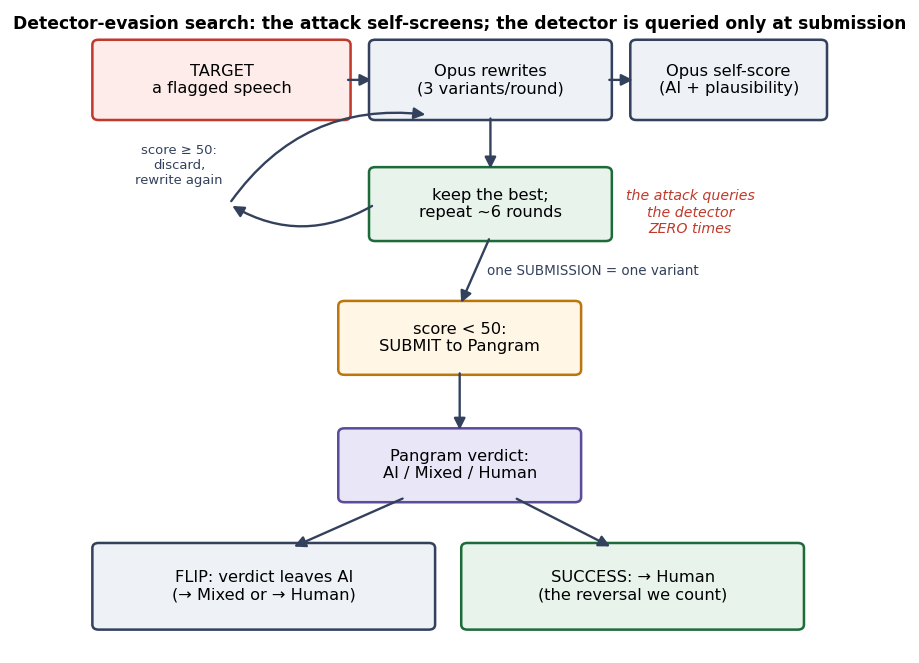
\includegraphics[width=0.85\linewidth]{bypass_search.png}
\caption{The detector-evasion search loop: the attack self-screens on the model\textquotesingle s own score and queries the detector only at submission; a \textbf{flip} is any verdict leaving AI, a \textbf{success} is a verdict reaching Human.}
\label{fig:bypass}
\end{figure}

\textbf{Three verdicts, and the two events we count.} Pangram returns one of three
labels, and the search can move a speech between them:

\begingroup\small
\begin{longtable}[]{@{}lp{0.28\linewidth}p{0.44\linewidth}@{}}
\caption{Pangram's three verdicts and the two events the search counts.}\label{tab:verdicts}\\
\toprule\noalign{}
Pangram verdict & meaning & counts as \\
\midrule\noalign{}
\endfirsthead
\toprule\noalign{}
Pangram verdict & meaning & counts as \\
\midrule\noalign{}
\endhead
\bottomrule\noalign{}
\endlastfoot
\textbf{AI} & the flagged starting state & --- \\
\textbf{Mixed} & "not confidently AI" & a \textbf{flip} (off AI) but \emph{not} a success \\
\textbf{Human} & "a person wrote this" & a \textbf{flip} \emph{and} a \textbf{success} --- the reversal we count \\
\end{longtable}
\endgroup

"Success" throughout means \textbf{reaching a clean Human verdict} --- the strict bar.
A "flip" is the weaker event of merely leaving AI; the two are different rates
and are never quoted interchangeably.

\textbf{The headline: a general-purpose model that is never shown the target
detector beats the commercial evasion industry by about tenfold.} The search loop (\cref{fig:bypass}) generates and screens variants against an \emph{Opus} self-score ---
a general intelligence, not the target --- and \textbf{Pangram is not in the loop}:
it sees only final submissions. Against the 13 commercial "humanizer"
services benchmarked in Pangram\textquotesingle s own technical report --- products built and
tuned \emph{against} detectors --- which get \textbf{2.31\%} of documents past it, this
blind-to-the-target search gets \textbf{22.5\%} of targets past it: \textbf{\(9.8\times\)}.
Against Pangram\textquotesingle s clean-conditions false-negative rate of 0.34\%, it is
\(66\times\).

That is the finding. The detector is not weak --- its specificity is 0 in 1,260
(\cref{sec:calibration}), and a single "make this sound human" prompt makes text \emph{more}
detectable, not less. But the gap between a purpose-built evasion product and
a frontier model told to try again is an order of magnitude in the frontier
model\textquotesingle s favour, and it will not narrow in the detector\textquotesingle s direction.

\textbf{Two rates, set by whether the attacker can test against the detector.} The
same search answers two threat models, and which number applies depends on one
thing --- whether the attacker can submit to the detector and retry:

\begingroup\small
\begin{longtable}[]{@{}lp{0.22\linewidth}p{0.16\linewidth}p{0.36\linewidth}@{}}
\caption{Bypass rates by whether the attacker may query the detector.}\label{tab:bypass-rates}\\
\toprule\noalign{}
rate & attacker\textquotesingle s detector access & value (two final runs) & the question it answers \\
\midrule\noalign{}
\endfirsthead
\toprule\noalign{}
rate & attacker\textquotesingle s detector access & value (two final runs) & the question it answers \\
\midrule\noalign{}
\endhead
\bottomrule\noalign{}
\endlastfoot
\textbf{per variant} & \textbf{none} --- one blind submission & \textbf{11.1\%} {[}5.5, 17.6{]} & a fire-and-forget attacker who cannot check their work \\
\textbf{per target} & \textbf{query + retry} (\(\leq\)18 attempts) & \textbf{22.5\%} {[}14.4, 33.5{]} & an attacker who submits, sees the verdict, and tries again \\
\end{longtable}
\endgroup

Both are realistic; they bracket the exposure. The gap between them is about
\textbf{\(2\times\)}. Everything below computes on the same two
final runs.

\textbf{The per-variant figure --- 11.1\%.} How often a single submitted variant
defeats the detector, for an attacker with no way to test candidates against
it first. On the two final searches, 38 of 341 submitted variants came back
Human; restricted to unambiguously AI-seeded originals it is 33/280 = 11.8\%.
The superseded first attempts produced 1 Human verdict in 120 variants (0.8\%);
folding them in gives \textbf{8.5\%} --- but averaging two biased samplings into the
denominator is not a cleaner estimate, only a more confusing one. The rate
rises when they are dropped, and we say so plainly.

\textbf{The intervals are clustered on text, and they are wide.} The 341 variants
are up to eighteen rewrites of each of 65 originals, so they are nowhere near
independent: treating each rewrite as its own trial gives a Wilson interval of
{[}8.2, 14.9{]}, about half the width it should be. The cluster bootstrap over
texts (20,000 draws) gives a \textbf{design effect of 3.40} --- the effective sample
is about 100 variants, not 341 --- and is what is quoted above. This is a
statement about repeated rewrites of one text adding little new information,
nothing more; it does not depend on any hypothesis about \emph{which} texts are
evadable (that question is exploratory --- see Appendix~\ref{app:superseded}). The
per-target figures need no such correction; they already carry one observation
per text.

\textbf{The operational figure --- 22.5\% per target, best method only.} An adversary
does not care how many drafts they discard; they care whether the speech they
wanted through got through. Taking only the \textbf{final search in each chamber}
and asking on what fraction of \emph{targets} at least one variant reached a clean
Human verdict:

\begingroup\small
\begin{longtable}[]{@{}lllll@{}}
\caption{Detector-evasion search yield per target.}\label{tab:bypass-yield}\\
\toprule\noalign{}
& searched & zero-yield & \(\geq\)1 Human & \(\geq\)1 at \texttt{fraction\_ai\ =\ 0.0} \\
\midrule\noalign{}
\endfirsthead
\toprule\noalign{}
& searched & zero-yield & \(\geq\)1 Human & \(\geq\)1 at \texttt{fraction\_ai\ =\ 0.0} \\
\midrule\noalign{}
\endhead
\bottomrule\noalign{}
\endlastfoot
NB v3 contrastive & 40 & 2 & 10 = 25.0\% & 10 = 25.0\% \\
GO all-31 uniform & 31 & 4 & 6 = 19.4\% & 5 = 16.1\% \\
\textbf{pooled} & \textbf{71} & \textbf{6} & \textbf{16 = 22.5\%} {[}14.4, 33.5{]} & \textbf{15 = 21.1\%} {[}13.2, 32.0{]} \\
\end{longtable}
\endgroup

\textbf{Roughly one flagged speech in five can be walked past the detector}, at a
budget of six rounds and three variants per round. One caveat on reading it as
a replication target: the NB v3 contrastive protocol was
designed by watching the blind attempt fail on the same texts, so its 25.0\% is
partly in-sample; the clean out-of-sample point is GO all-31\textquotesingle s \textbf{19.4\%}, a
different chamber under a uniform draw. That the two land close is mild
evidence the method travels rather than fits --- but the honest single
replication expectation is "\(\approx\)19--22\%, wide interval". The in-sample element is
left in deliberately: an iterating attacker who learns from failed attempts is
the realistic threat, and the v3 protocol was specified from the mechanism,
not from per-text outcomes.\footnote{\texttt{BYPASS\_METHODOLOGY.md}.}

\textbf{The evasion is not Pangram-specific --- but the alternatives barely detect
this genre to begin with.} Scoring the 341 final variants and their 65
originals on three open detectors it never targeted --- Fast-DetectGPT,
Binoculars, and the DetectLLM log-rank ratio, each thresholded at the 5\%
false-positive point on 1,255 pre-2022 human controls --- \textbf{79\% of the
Pangram-evading variants evade all four detectors at once}, and each open
detector individually flags only 6--10\% of them. The transfer is nearly
complete, but the honest reason is two-sided: these zero-shot detectors are
weak on institutional prose in the first place, catching just 26\%
(Fast-DetectGPT), 17\% (log-rank) and 6\% (Binoculars) of the un-rewritten
machine text Pangram flagged --- the same collapse \cref{sec:related} documents on this
register. So the multi-detector test cannot show a \emph{strong} evader
defeating \emph{strong} alternatives; what it shows is that the one calibrated
detector\textquotesingle s verdict is not idiosyncratic --- a rewrite tuned past it is past
the others too --- and that no detector available to us holds this genre
under directed effort.\footnote{\texttt{python\ score\_\allowbreak{}multistat.\allowbreak{}py} (Fast-DetectGPT, Binoculars and LRR
  from one committed Falcon-pair pass) on the assembled variants and
  controls, then \texttt{python\ detector\_\allowbreak{}transfer.\allowbreak{}py}. Thresholds are each
  detector\textquotesingle s 95th control percentile; the per-run split is in the output
  (the uniform GO run evades harder --- 1--4\% open-detector flags --- than the
  contrastively-seeded NB run at 9--14\%).}

\textbf{The denominator is targets searched, not targets that yielded a variant.}
The search submits a rewrite to Pangram only when its Opus proxy score drops
below 50, and six of these 71 targets ran four to six full rounds without ever
producing one. Those are attack failures --- an adversary who cannot produce a
candidate their own proxy will submit has not got that speech past anything ---
so they belong in the denominator. Counting only targets that yielded makes
the rate conditional on the attack having already half-succeeded, and gave
24.6\% where the answer is 22.5\%.

Those six are not evidence that the text cannot be disguised. They establish
that \emph{this} search, at this budget, did not manage it --- and the search had
converged, so further draws from the same process would probably not have
helped either. Whether a \textbf{different method} would is a separate question and
an untested one: better contrastive exemplars, a rewriter fine-tuned against
the detector, or a human editor are all outside what was tried.

The two chambers give 25.0\% (n = 40) and 19.4\% (n = 31) --- \textbf{consistent, but
with intervals far too wide to establish that they agree}: the 5.6-point gap
carries a 95\% interval of roughly {[}\(-17\), +25{]} points, equally compatible with
one chamber\textquotesingle s rate being half or double the other\textquotesingle s. What is
more than a restatement of the wide interval is that the two chambers\textquotesingle{}
\emph{humanising playbooks} flatly contradict each other --- they agree on repetition
and unglossed idiom and disagree on sentence rhythm --- so if the rates do turn
out to transfer, the edits that produce them do not.

\textbf{Against 0 AI labels in 1,260 genuine pre-AI controls (\cref{sec:calibration}).} That is what
makes the reversals worth reporting: they are movements \emph{into} a class the
detector otherwise reaches zero times out of 1,260. This is not a detector
that is merely noisy at the boundary --- it is one with a hard specificity floor
that a directed search nevertheless walks text across.

\textbf{Naming the quantity precisely, because the comparison is easy to get wrong.}
Ours is an \textbf{induced false-negative rate} under attack, and it is \emph{not} the
same measurement as a vendor\textquotesingle s published FNR, for two reasons that must travel
with the number. First, ground truth is a Pangram verdict on the \emph{original},
not known authorship --- a "false negative" here means the detector reversed
itself on text it had flagged, not that a machine demonstrably wrote it.
Second, the variants are the surviving output of a search that optimised
against a correlated proxy, so this is a rate under adversarial pressure
rather than under clean conditions.
The false-negative rates in play, and what each one is measured on:

\begingroup\small
\begin{longtable}[]{@{}p{0.22\linewidth}p{0.20\linewidth}p{0.50\linewidth}@{}}
\caption{The bypass rates, disambiguated.}\label{tab:bypass-summary}\\
\toprule\noalign{}
measurement & rate & what it is \\
\midrule\noalign{}
\endfirsthead
\toprule\noalign{}
measurement & rate & what it is \\
\midrule\noalign{}
\endhead
\bottomrule\noalign{}
\endlastfoot
Pangram 4, clean & 0.34\% & FNR, known-AI text, vendor-reported \\
Pangram 4, 13 humanizer services & 2.31\% & FNR under commercial evasion, vendor \\
Pangram 4, BLADER de-AI agent & 0.43\% & FNR under agentic evasion, vendor \\
Pangram 4, Epoch AI Style Imitation & 2.86\% & FNR, doc-level, adversarial, vendor\footnote{2.86\% (17/594) is Pangram 4\textquotesingle s
  document-level false-negative rate on the \textbf{Epoch AI Style Imitation}
  benchmark (the Pangram 4 report\cite{pangram4}\textquotesingle s own Table 23). The Perkins benchmark\cite{perkins2024}
  (their Table 22) reports mean accuracy --- a different unit, with Pangram at
  \textasciitilde5.9\% miss on the manipulated set --- which is not FNR-comparable and is not
  tabled here.} \\
\textbf{this study, per variant} & \textbf{11.1\%} & \textbf{induced FNR, one blind submission (no attacker detector access) --- \(4.8\times\) the humanizers} \\
\emph{this study, per target} & \emph{22.5\%} & \emph{induced, attacker may query and retry (\(\leq\)18 attempts) --- \(9.8\times\) the humanizers} \\
\end{longtable}
\endgroup

(and, later in the same paragraph, replace the Rice sentence with:) Rice 2026\textquotesingle s Australian-Hansard \textasciitilde8\% is deliberately \emph{not} a row in this table, though the numeric coincidence invites it: that figure is a false-\emph{positive} rate on 50 pre-ChatGPT speeches, measured on an LLM judge rather than on Pangram (\cref{sec:related}) --- a column of false-negative rates is no place for it.

\textbf{The per-variant row is the one commensurable with the vendor rows}, which
are also document-level FNRs on one adversarially prepared submission. The
difference is method, not accounting: our submissions are the survivors of an
Opus self-screen, i.e. a stronger attack than a single humanizer pass, which
is why 11.1\% exceeds the 2.31\% commercial rate. This is a comparison of point
estimates: clustered on text the per-variant interval runs {[}5.5, 17.6{]}, so the
adversarial vendor figures at 2.31--2.86\% sit below our estimate but inside its
lower tail --- the ordering is secure, its margin less so. The per-target row is
italicised because it allows up to eighteen attempts per document, and no
published benchmark grants that; it is the right number for exposure, the
wrong number for a detector comparison. The Rice row is included because the
numeric coincidence invites a comparison that does not exist: his \textasciitilde8\% is a
false-positive rate on 50 pre-ChatGPT speeches, measured on an LLM judge
rather than on Pangram (\cref{sec:related}). The vendor rows are vendor-reported on
undisclosed test data and should be read as such; independent evaluations
(RAID, Dugan et al. 2024; Weber-Wulff et al. 2023) consistently find detectors
fail toward false negatives under obfuscation, which is the direction our
result also points.

\textbf{Both rates move with effort, and the two bars must not be confused.} A
\emph{flip} (leaving AI for Mixed-or-Human) is far easier than a \emph{success}
(reaching Human), so the flip rate is always the larger number and is not
comparable to the per-variant success rate. Stating both explicitly for the
New Brunswick protocol change: the blind first attempt flipped \textbf{10\%} of
variants (4/40) and reached Human on \textbf{2.5\%} (1/40); the contrastive search
flipped \textbf{28\%} (59/212) and reached Human on \textbf{13.7\%} (29/212). Effort
raised both bars, and by \emph{more} on the success bar (\(5.5\times\)) than on the flip bar
(\(2.8\times\)). And at the target level, if merely "soften off AI" is the goal, 17 of
38 New Brunswick targets (\textbf{45\%}) cleared it. So the success rates --- 11.1\%
per variant, 22.5\% per target --- bound what these searches achieved, not what
is achievable; the flip rates show how much more room a laxer bar leaves.

\textbf{Which texts evade is exploratory and stays out of the register above.} Are
borderline originals --- those the detector was least sure about --- the evadable
ones? The seed-verdict split and the band gradient both point that way weakly
and neither survives a test (Fisher p = 0.735 on the seed split; a non-monotone
gradient on \textasciitilde53 variants per band). This is the arm\textquotesingle s most speculative
question, it should not be quoted as a finding, and the numbers and a retracted
earlier version of it are in Appendix~\ref{app:superseded}. The one firm negative: 28\% of
Mixed-seeded variants moved the \emph{wrong} way, to AI --- a directed search against
this detector is not monotone.

\textbf{The label and the score disagree at the boundary, and the interface hides
it.} Of the 9 Government Orders reversals, one (\texttt{ga033}) came back \textbf{Mixed at
\texttt{fraction\_ai} 0.67} on re-scan rather than Human at all, and another
(\texttt{ga092}) was Human at 0.10 rather than 0.0 --- about 11\% verdict instability on
the same text and the same model. New Brunswick showed none: all 30 of its
Human labels re-scanned at exactly 0.0. The dashboard reports a categorical
label, so a user reads "Human" as "a person wrote this"; the continuous score
underneath sometimes says something weaker. Both numbers are therefore reported
throughout this study, and the gap between them --- half a percentage point
pooled --- changes no conclusion here.

\textbf{Evasion-directed rewriting does not measurably change deliberative
quality.} Two paired arms, 63 within-text pairs, blinded and interleaved,
graded on the same v2b DQI rubric: stage 3 is 38 New Brunswick pairs (the v3
ladder variants), stage 4 is 25 Government Orders pairs from the \textbf{GO
Opus-selected run} --- not the GO all-31 arm of the bypass section above, with
which it shares no segments. Named precisely because of what the verdicts
show: \textbf{61 of the 63 graded rewrites did not clear the detector} (stage 3:
AI 29 / Mixed 7 / Human 2; stage 4: AI 23 / Mixed 2). What is measured is the
effect of rewriting \emph{under an evasion instruction}, not of successful evasion
--- the selection was by the Opus proxy, not the Pangram outcome, so this graded
set is not conditioned on failure. The complementary arm, graded ON the
Pangram outcome (the successful reversals), is stage 5 below. Within-text pairing holds content, speaker and occasion fixed by
construction, so these are the raw paired differences --- the design\textquotesingle s own
estimand, needing no covariate. \textbf{Every dimension is null on both.}\footnote{\texttt{cd\ quality\_expansion\ \&\&\ python\ analyze\_stage3.py\ {[}RUNDIR{]}} and
  \texttt{python\ analyze\_stage3.py\ -\/-key4\ {[}RUNDIR{]}}; values cached in
  \texttt{results\_stage34.json}, which now also caches \texttt{r\_words} per dimension.
  The grading transcripts (stage 3 run \texttt{wf\_b9bbcff8-1a7}, stage 4
  \texttt{wf\_7516f16c-386}, on the grading machine) were recovered 2026-08-20 and
  their id-keyed rows are committed as \texttt{stage3\_\allowbreak{}grades\_\allowbreak{}by\_\allowbreak{}id.\allowbreak{}json} /
  \texttt{stage4\_\allowbreak{}grades\_\allowbreak{}by\_\allowbreak{}id.\allowbreak{}json} beside the raw archives, with the stage-3
  table verified to reproduce digit-for-digit; the script needs a run
  directory, so pass one (or rebuild from the committed rows). Quoted column is the \textbf{raw paired difference},
  humanized \(-\) original, within text. \texttt{-1} (inapplicable) pairs are excluded,
  which is why the two sentinel dimensions have smaller n (12 and 12 in
  stage 3; 18 and 16 in stage 4).}
What the pairs can exclude is bounded and stated:
detectable effects run roughly \(\pm\)0.12--0.26 per dimension for stage 3 ---
commensurate with the study\textquotesingle s own headline effects (+0.22 to +0.29, stage 2)
--- so these nulls say the evasion edit produces nothing dramatic, not that it
produces nothing at the scale the study elsewhere reports. Made formal, the
bound holds where the n does: stage 3 shows TOST equivalence within \(\pm\)0.22
on five of seven dimensions (the two applicability-gated respect dimensions
run too thin at n = 12), stage 4 on three of seven --- the rest are bounded
only at headline scale, exactly as the MDE statement says.\footnote{\texttt{python\ tost\_\allowbreak{}equivalence.\allowbreak{}py} --- SESOI fixed at \(\pm\)0.22 raw points,
  the low end of the stage-2 headline range, chosen once and applied to
  every equivalence statement in the paper; two one-sided tests on the
  committed estimators.} None of the 28
paired cells reaches nominal significance, which is how a true null behaves
under many looks. And the paper\textquotesingle s quality conclusion does not rest on these
arms: it is carried jointly by stages 1 and 2 (wild text, two label
sources), stage 5 (successful evasions), and stage 6 (never-reviewed
continuations, where frontier models \emph{beat} the human twins on form) --- four
different contrasts agreeing.
The paired cells, dimension by dimension:

\begingroup\small
\begin{longtable}[]{@{}lll@{}}
\caption{Paired within-text quality comparisons (stages 3 and 4).}\label{tab:quality-paired}\\
\toprule\noalign{}
dimension & stage 3 (n=38) & stage 4 (n=25) \\
\midrule\noalign{}
\endfirsthead
\toprule\noalign{}
dimension & stage 3 (n=38) & stage 4 (n=25) \\
\midrule\noalign{}
\endhead
\bottomrule\noalign{}
\endlastfoot
justification & +0.05 (t +0.6) & +0.16 (t +1.7) \\
common\_good & \(-0.05\) (t \(-0.8\)) & 0.00 (t 0.0) \\
respect\_groups & \(-0.08\) (t \(-1.8\)) & +0.04 (t +1.0) \\
respect\_demands & \(-0.08\) (t \(-0.6\)) & 0.00 (t 0.0) \\
respect\_counterargs & +0.33 (t +1.8) & +0.12 (t +1.0) \\
constructive & 0.00 (t 0.0) & \(-0.12\) (t \(-1.8\)) \\
evidence & +0.03 (t +0.4) & +0.08 (t +0.7) \\
\end{longtable}
\endgroup

\textbf{Stage 5 grades the successful evasions themselves, and finds the same
null.} Conditioning on the outcome --- the complement of stages 3/4 --- every
rewrite that reached a Human verdict (39 variants across 15 targets, one
target\textquotesingle s original text unavailable and dropped) was graded blind against its
original on the same v2b rubric, two independent passes (inter-pass exact
agreement 79--100\%). No dimension moves at either level:

\begingroup\small
\begin{longtable}[]{@{}lll@{}}
\caption{Quality of successful evasions versus their targets, by dimension.}\label{tab:quality-evasion}\\
\toprule\noalign{}
dimension & variant (n=35) & target (n=15) \\
\midrule\noalign{}
\endfirsthead
\toprule\noalign{}
dimension & variant (n=35) & target (n=15) \\
\midrule\noalign{}
\endhead
\bottomrule\noalign{}
\endlastfoot
justification & \(-0.14\) (t \(-1.7\)) & \(-0.03\) (t \(-0.2\)) \\
common\_good & +0.01 (t +0.3) & +0.03 (t +0.4) \\
respect\_groups & +0.04 (t +1.0) & +0.10 (t +1.2) \\
respect\_demands & \(-0.01\) (t \(-0.6\)) & 0.00 (t 0.0) \\
respect\_counterargs & +0.11 (t +0.9) & +0.10 (t +0.4) \\
constructive & +0.03 (t +1.0) & +0.07 (t +1.0) \\
evidence & \(-0.01\) (t \(-0.2\)) & +0.04 (t +0.3) \\
\end{longtable}
\endgroup

The lone lean --- justification at variant level (t \(-1.7\)) --- collapses on
aggregation to targets (t \(-0.2\)), a within-target artifact of multiply-graded
targets, not a cost. So the two arms bracket the claim: \textbf{evasion-directed
rewriting is null (stages 3/4) and evasion-ACHIEVING rewriting is null (stage
5).} (A note the DQI judge\textquotesingle s own \texttt{ai\_guess} adds: it rated the successful
evaders 36/100 against 40 for the human originals --- barely less AI-like --- so
the two detectors disagree on this set even as neither finds a quality
difference.\footnote{\texttt{stage5\_scores.json}, \texttt{PREREG-\allowbreak{}stage5-\allowbreak{}successful-\allowbreak{}evasion.\allowbreak{}md}.})

\textbf{On length, which we do not adjust away --- and which does not replicate.}
Stage 4\textquotesingle s rewrites run about 29 words longer than their originals; stage 3\textquotesingle s do
not (mean \(-1.3\)). Within stage 4, justification does move with length, at
\textbf{r = +0.33}. That is the largest correlation on the board and it points the
way the length story predicts.

It does not survive the other stage. In stage 3 the same correlation is
\textbf{r = \(-0.24\)} --- longer rewrites justify \emph{less} --- and stage 3 is where the
estimate is better identified, its word deltas running both directions with sd
38 against stage 4\textquotesingle s one-sided 14. Neither reaches significance (p = 0.11 and
p = 0.15). \textbf{A relationship that changes sign between two arms of the same
design is not a relationship}, and the tidy explanation that justification\textquotesingle s
stage-4 drift "was length" fails on the data rather than on the statistics.

We report the correlation rather than removing it, because length is not a
confound here in any case. On this rubric a longer passage genuinely has room
to justify more, and a member with a longer slot could earn the same points the
same way. Adding justification by adding words is a real strategy, not an
artifact of one; partialling it out would treat a route to quality as a
nuisance parameter.\footnote{A length-adjusted column would be the natural check here, and its
  absence is deliberate: that column is the regression intercept at a word
  delta of zero, and 24 of the 25 stage-4 deltas are strictly positive --- a
  zero delta sits 2.1 sd outside the sample with one observation there,
  giving an intercept VIF of 5.43 and inflating the standard error \(2.3\times\),
  so any sign flip it showed would be extrapolation. The design is
  within-text paired: content, speaker and occasion are already fixed by
  construction, and there is nothing for a covariate to control.}

\textbf{What this means for the prevalence number.} Evasion is real and clears
the detector on roughly one flagged speech in five under directed search ---
so 9.0\% is a floor on \emph{use}: it measures undisguised machine drafting, and
disguised drafting exists above it. The quality clause is a separate claim,
and one-directional: no measured arm shows a deliberative-quality \emph{cost} to
the evading rewrite --- the paired nulls bound only headline-scale effects
(their minimum detectable effects), but every powered result runs favourable --- which is
what the norms argument needs; it does not claim the edit adds nothing. But it is not free in effort:
it took a frontier model, contrastive exemplars mined from matched human text,
and a multi-round search scoring three replicates per variant. A single
"make this sound human" prompt does the opposite --- instructed rewriting \emph{raises}
Pangram\textquotesingle s score, and human text pushed through the same ladder went from 11.7
to 60.2. The gap between "a detector can be beaten" and "a detector is easy to
beat" is the whole of that apparatus.

\begin{center}\rule{0.5\linewidth}{0.5pt}\end{center}

\section{Discussion}\label{sec:discussion}

This study set out to count machine-drafted speech and found, behind the count, a register with a thirty-year human history. The count stands, and it belongs to the calibrated detector alone: \textbf{at least 9.0\% of words} in current legislative speech are machine-drafted, spread fourfold across chambers and concentrated where procedure permits preparation. The transparent lexical register corroborates it where the two instruments\textquotesingle{} inferences overlap --- the genre ladder --- and carries what the detector cannot: the history and the social structure. That register is the older finding: rising since 1994--96, strongest in later-born members, shaped like the office --- peaking at its insulated middle --- and installed, on the machine side, at exactly the post-training stages tuned toward human demonstrations and preferences. Machine intelligence did not invent this register of accountability without authorship --- it inherited it, and this study measures the inheritance.

What follows from that depends on what detection can actually do. \cref{sec:evasion} is
usually read as a result about one detector. It is better read as an
instance of a general limit, and the generalisation changes what the rest
of the study is for.

\subsection{Any check the attacker can score against is an optimisation target}\label{sec:disc-limit}

Point a general-purpose model at its own output, tell it to try again, and it will beat any check it can score against. This is not a claim about Pangram, and it is not a defeat theorem for fixed checks: it is the supportable form --- a check whose output, or a correlated proxy for it, the attacker can query is an optimisation target, and the attacker carries a quality constraint it can itself satisfy. The 22.5\% in \cref{sec:evasion} is a lower bound on that adversary class, measured at its weakest member.

Our own numbers are the \emph{weak} instance. The search never queried the detector
it was evading: it optimised against an Opus proxy, tested on Pangram only at
the end, used roughly eighteen attempts per target, and involved no
fine-tuning, no gradients, and \textbf{no query access to the detector during the
attack} (the detector\textquotesingle s only role was labelling pre-2022 text human, to build
contrast exemplars). 22.5\% of
targets cleared is what that buys. An adversary who can query the check
directly is hill-climbing the actual objective, and there is no reason to
expect the ceiling to be near where we stopped.

\textbf{Two scoping notes, because the argument can be overextended.} Inferring
\emph{future} checks is weaker than defeating present ones --- you cannot optimise
against features you cannot anticipate. And the limit applies to \textbf{post-hoc
statistical detection of unmarked text}, which is a different problem from
provenance asserted at generation time.

\subsection{Where the norms argument actually lands}\label{sec:disc-norms}

Detection fails against adversaries and works against everyone else. That is
not a small residual: the 9.0\% in \cref{sec:prevalence} exists precisely because nobody
currently bothers to evade, or the undisguised register signature would not be
there to find. \textbf{Detection is a norms instrument, not a security instrument} ---
locks, not vaults. It raises the cost of casual undisclosed use and does
nothing against motivated use, and that is a coherent thing for a chamber to
want. It is also what lets 9.0\% stand as a measurement of disclosed-by-default
behaviour while conceding the limit above entirely.

The better version of the norms instrument is not a sharper detector but a
\textbf{signature the generator puts there on purpose}. Anthropic began embedding
"an imperceptible watermark directly into the text itself" for Claude models
launched on or after \textbf{2 August 2026}, with retrofitting of existing models in
progress, across all its products and its AWS, Google Cloud and Microsoft
distribution; generated image files additionally carry C2PA-signed provenance
metadata. Detection is not yet public --- the company says it is "working to
enable users and other third parties to detect Claude\textquotesingle s embedded watermarks",
with technical documentation forthcoming. Google DeepMind\textquotesingle s SynthID-Text
(Dathathri et al., \emph{Nature} 2024) is the deployed precedent.

\textbf{The durable argument for hiddenness is not robustness --- it is minimal
interference with the content.} This is worth stating carefully, because the
obvious argument is the wrong one. One could say a secret-keyed mark cannot be
hill-climbed without query access to the verifier, which is exactly the
situation our search was in and the reason it needed eighteen tries. True, but
fragile: it erodes the moment the detector is released, and released detectors
are the whole point of a transparency measure. Anthropic\textquotesingle s own documentation
concedes the robustness half --- marks may not survive text that is "heavily
edited, paraphrased, translated, or mixed", and short passages may carry no
reliable signal.

The property that never goes away is that an invisible mark \textbf{costs the reader
nothing even after the detector is public}. A visible disclosure label
degrades the artifact, invites removal, and is trivially stripped; an
imperceptible one imposes no cost on the text and survives ordinary copying
between applications. Image watermarking is the settled analogy: easy to crop
or inpaint away, universally deployed anyway, and useful precisely as a norm
rather than a lock.

\textbf{Bypassability is therefore not a defect here --- it is the category.} Zhang
et al., \emph{Watermarks in the Sand}, give an impossibility result for strong
watermarking against an attacker with a quality oracle and a perturbation
budget, close to the setting we ran; paraphrase degrades token-level marks
(Sadasivan et al. 2023, with Kirchenbauer et al. 2023b making survival a
function of marked-token count). None of that refutes the instrument. It
establishes that a watermark is a norms instrument and not a security
primitive, which is the same thing \cref{sec:evasion} establishes about detection, and both
are still worth having for the same reason locks are.

Two limits that do bite, and neither is about robustness:

\begin{itemize}
\tightlist
\item
  \textbf{It requires the generator to cooperate.} Open-weight models will not mark
  their output, so this prices casual frontier-API use and does nothing about a
  local model.
\item
  \textbf{A mark attests presence, never absence.} Unmarked text proves nothing,
  which means watermarking can support a disclosure norm but can never
  underwrite an accusation.
\end{itemize}

And the fallback people reach for when a detector is unavailable --- their own sense of whether text "reads like a person" --- is worse than unreliable on adversarial input; it is anti-correlated with the truth. Asked to judge AI-likeness by register, a frontier reader flagged 13 of 35 genuine human floor speeches and only 5 of 35 machine rewrites that had been optimised against a detector (\cref{sec:evasion} stage 5): adversarial optimisation removes exactly the tells gut judgment keys on, so the errors of a vibes-based adjudicator concentrate on the \emph{unoptimised} --- ordinary speakers who ran their words through nothing. As machine-assisted text spreads, register stops carrying authorship information, and an institution still adjudicating authenticity by feel is grading noise. That the errors then fall hardest on the unassisted --- that machines will overtake humans at seeming human to humans --- is a conjecture resting on one unblinded, lineage-correlated judge on 35 texts, and it stays a conjecture until it happens (see the future-work item below). We state it because, after watching machines overtake human performance at task after task, we do not expect this one to be the exception.

\subsection{Policy context}\label{sec:policy}

A 22-chamber scan found \textbf{zero chambers requiring AI-drafted text to be
disclosed in the record, and none forbidding AI drafting.} Where rules
exist they are IT-security instruments issued by Clerks and CIOs, not rules
of authorship. The structural pattern: \textbf{where a Clerk governs staff, rules
are detailed; where members govern themselves, there is nothing.}

Strictest is the US House (HITPOL 8). The UK is the only chamber to address
the question directly, and resolves it permissively --- AI-generated content in
proceedings is the member\textquotesingle s own, "protected by privilege regardless of the
tools used to produce that material." The only Speaker\textquotesingle s ruling anywhere in
scope is Alberta, 2 December 2025: asked to extend the anti-staff-written-
speeches rule to AI, Speaker Cooper ruled \textbf{"ChatGPT is not staff."}

Coverage is partial for NI, Manitoba, PEI and South Australia --- absence of
evidence, not evidence of absence. Among the six chambers where the scan is
high-confidence, Saskatchewan, Nova Scotia and Newfoundland \& Labrador are
equally solid nulls --- no AI-specific rule found.\footnote{\texttt{ai\_policy\_scan.md}; figures unverified against primary
  sources.}

The rules will lag; the measurement need not. What this study prototypes ---
a standing, machine-executed audit of an open record, cheap enough to rerun
every sitting --- is the natural complement to whatever disclosure rule a
chamber does adopt. And it generalises: the same instruments that measure
how much machine text enters a record can measure whose register a model
was tuned to reproduce, which is the form of oversight the substitution
worry (\cref{sec:intro}) actually calls for.

\subsection{The substitution, and why our null is the argument for it}\label{sec:disc-substitution}

If provenance is the wrong thing to spend effort on, the question is what to
spend it on instead. The answer available from this study is: \textbf{check the work
directly.}

The case rests on \cref{sec:quality}\textquotesingle s primary finding and is independent of evasion: speech classified as machine-involved grades \textbf{better-formed, not worse-engaged} on the DQI. Policing authorship therefore does not protect quality, because the text flagged for machine involvement is not where this rubric finds a quality deficit. The narrower conclusion is the useful one: \textbf{quality assessment is not a usable proxy for provenance, and provenance is not a usable proxy for quality.} The DQI associations with the machine label are real but small, partly exposed to judge leakage, and positive where they survive; they neither identify authorship nor support treating machine involvement as a quality failure.
Two dimensions do run lower on the machine side, and they are the right targets for improvement rather than counterexamples: wild flagged speech is about half as likely to contain anything to engage with (the applicability split, \cref{sec:quality} --- a raw contrast, not genre-adjusted), and machine text sits below humans on checkable specifics (stage 6) --- with the continuation evidence attributing the applicability collapse to weaker tools in use, not to machine assistance as such (opus-class continuations carry as much to engage with as the humans). Both deficits are visible only because the work is checked directly, which is the argument.

The composite weights the seven DQI dimensions equally --- the index\textquotesingle s conventional additive form --- rather than by any measured optimum; tested, the weighting matters and the direction survives it. The seven dimensions are not one factor (the first principal factor of their polychoric matrix carries 32--33\%), and that factor loads on the respect dimensions rather than on the well-formedness dimensions that carry the machine advantage --- so re-running the stage-2 contrast on the factor-weighted latent score cuts it from +0.195 (t 5.65) to +0.076 (t 1.71): still positive, no longer significant. The honest statement is that "better-formed" is dimension-specific --- justification and evidence carry it --- and any weighting that emphasises engagement over form puts the composite contrast at the margin, which is one more reason the paper\textquotesingle s claims are stated per dimension rather than from the index.\footnote{\texttt{python\ quality\_\allowbreak{}latent.\allowbreak{}py} --- polychoric matrix on the seven
  dimensions (two-step: thresholds from the marginals, pairwise \(\rho\) by ML
  over bivariate-normal rectangle probabilities; sentinel \(-1\)s as
  missing; the Spearman version is printed alongside and agrees), first
  principal factor, latent = loading-weighted mean of available
  standardised dimensions, contrasts re-run with the committed columns\textquotesingle{}
  own estimators (stage 1 per sd of screen score, where the factor
  weighting flips the weak positive to a weak \(-0.038\), t \(-1.71\); stage 2
  AI/Mixed vs Human with chamber FE, HC1). A full graded-response IRT
  is the remaining refinement.}

The reliability statistics cannot carry this claim by themselves --- a consistently biased judge would also reproduce itself perfectly. What carries it is validity evidence: the rubric\textquotesingle s calibration anchors are the instrument authors\textquotesingle{} own published codings, so the scale is theirs rather than the judge\textquotesingle s; the one dimension where judge-suspicion moves the result is identified and quarantined rather than averaged in (respect\_groups; Appendix~\ref{sec:judge-leakage}, \cref{sec:quality}); and across stages the judge\textquotesingle s AI-guess and its quality scores move independently in both directions --- higher form under suspicion in the wild pools, lower for weak models and higher for frontier ones in stage 6.

The paired evasion arms add a separate, secondary reassurance for anyone worried about the arms race specifically: rewriting under evasion pressure did not move any of the seven dimensions across 63 within-text pairs, and neither did the 39 rewrites that actually cleared the detector when graded on their own (\cref{sec:evasion} stage 5). A body that measures quality directly need not fear that evasion --- attempted or achieved --- degrades the metric it watches.

And it is now cheap in a way it has not been before. The instrument\textquotesingle s
repeat reliability sits at or above the published human inter-coder bar, on
a rubric with published human codings as anchors. Twenty
years ago the Discourse Quality Index required trained coders and bounded any
study to a few hundred speeches. We graded 1,522 in the main arms without
trained coders. That capability arrived with the same technology that broke
detection, which is the substitution in one sentence: the machine that made
provenance unmeasurable made quality measurable.

Deliberation is judged on the artifact, so checking the artifact suffices.
Education is not judged on the artifact: there the text is a proxy for what
is in someone\textquotesingle s head, and a proxy that can be generated is no proxy at all. That case needs a \textbf{more rigorous proof of
understanding}, and machine intelligence supplies the means as well as the
problem --- adaptive examination against a person\textquotesingle s \emph{entire} corpus of work, with
provenance and time-on-task as evidence rather than the text alone.

Two costs to state plainly. Process and timing data are themselves spoofable,
so this is an escalation and not a resolution. And "analyse the student\textquotesingle s
entire corpus" is a surveillance instrument before it is an assessment
instrument; the version worth building is the one that is legible to the person
being assessed.

\subsection{The measure against the market\textquotesingle s measure}\label{sec:market-measure}

The classification result carries a point beyond stratification. The
classical scales are the market\textquotesingle s own summaries of occupational position ---
ISEI is fitted to the education--income path by construction, and the
categorical schemas were validated against employment relations --- while
the folk ladder was built blind: model-elicited from aggregated human
expression, no outcome visible, its ordering registered before any join.
On this outcome the blind measure absorbs the categorical schema in the
joint model (\cref{sec:four-predictors}) --- and, with the anchors joined, holds against the
fitted continuous scales too: beside the study\textquotesingle s covariates, ISEI and wage
quartiles collapse while the folk block stands, and more than half of each
level\textquotesingle s variance lies off the education--earnings plane entirely (\cref{sec:occupation}).
A classification built blind recovered social-structural information the
market-fitted scales demonstrably do not carry. That
is the live instance of the change this paper keeps meeting --- structure
that institutions summarised lossily, because tracking it was uneconomic,
becoming directly measurable.

What the comparison does not establish should be stated with the same
care, because a further reading is tempting and rests on an assumption:
that the recovered structure is \emph{more useful} than what the market prices
--- that position, as the register instruments it, is the referent the
market\textquotesingle s scales summarise lossily. One reading supports that: a market
has no physical existence of its own; it is itself an aggregation
mechanism whose claim is to reflect the social structure, which the
register instruments directly. But there is a counter-reading, and it is
the paper\textquotesingle s own hypothesis: social structures --- spoken registers among
them --- often function to \textbf{mask} disparities in productivity, and on
that reading the register instruments the veil rather than the referent,
so the measure and the market are pricing different things. The two
readings disagree about what was measured and agree that it was measured
--- and the check that discriminates them is already registered (Appendix~\ref{app:future},
item 32): tie register intensity to productivity and success measures.
Signaling drag --- register predicting \emph{worse} real outcomes --- favours the
masking reading; register tracking outcomes the market\textquotesingle s summaries miss
favours the lossy-summary reading. Either way, the measurement point
survives: the structure was there, untracked, and a blind machine measure
picked it up.

And a weaker form of the larger point survives the dispute between
readings entirely, because it does not depend on what the register refers
to. The standing defence of the market as social oracle has never been
that it measures well; it is that nothing measures better --- the best of
bad options. What this result demonstrates is the arrival of another kind
of option: a bespoke measure, elicited blind from aggregated human
experience at trivial cost, preregistered, and better than the fitted
schemas on the first outcome it was pointed at. Whether it found referent
or veil, the capability generalises --- measures like this can now be built
per question, blinded by construction, and checked --- and every one built
weakens "best of bad options" as an argument for reading social structure
off prices alone.

\subsection{Measuring the human contribution against an automated counterpart}\label{sec:disc-human}

The most promising direction, and the least developed. Generate what a fully
automated system would produce given the same task and context; the human
contribution is the residual. This is the marginal-product definition done
properly, and it is measurable today.

\textbf{The baseline must move.} The obvious objection is that the residual shrinks
as models improve, and the obvious fix --- freeze a model vintage --- is wrong. It
reproduces the error the current debate already makes, where contributions
relative to dumb computers are treated as obviously legitimate and anything
touching an LLM as obviously suspect. \textbf{The goalpost should move by
construction, always incorporating the latest technology}, because that is
what contribution means: what you added over the best available alternative. A
shrinking residual is correct measurement, not measurement decay. Nobody
credits long division done by hand.

The one thing worth recording is \emph{which} baseline a given measurement was taken against --- metadata that keeps an old measurement interpretable, not a fixed target. This moves for the same reason measured imitation lags collapse, and is collapsing for the same reason --- it is not literally the same quantity those lag measurements capture.

A scope condition worth stating, because the whole moving-baseline proposal
assumes it: the measure is affordable only where the cost of reproducing an
intellectual result under it is close to zero. Frontier models and
frontier-grade processes may always sit out of its reach, or be sampled only
sparsely. But the majority of \emph{average} human intellectual activity is well
within it --- and the case that matters most is education, in schools and
workplaces, which will have to teach people to work productively with advanced
intelligences and can use a continuously-recalibrated baseline to measure
whether they are.

\begin{center}\rule{0.5\linewidth}{0.5pt}\end{center}

\subsection{Limits}\label{sec:limits}

\begin{itemize}
\tightlist
\item
  \textbf{Prevalence is a floor.} Detectors see undisguised machine text. A
  directed search clears the detector on 11.1\% of variants and \textbf{22.5\% of
  targets} (\cref{sec:evasion}), so 9.0\% is a lower bound. How much of a lower bound is
  not estimable from this design: we can measure how often evasion succeeds
  when attempted, not how often it is attempted.
\item
  \textbf{The evasion rate is an upper bound on our own effort, not on anyone\textquotesingle s.}
  Four runs over two days with a frontier model. A staff tool refined over
  months, or a local model fine-tuned against the detector, is a different
  adversary and we did not test one.
\item
  \textbf{Tasmania is uninterpretable} and excluded. All twenty-one screened
  chambers now run the diagnostic (it previously globbed only the provinces;
  CA-FED, US House and US Senate were added --- CA-FED flat, the two US chambers
  a gradual multi-decade climb with no discrete step). The twenty pooled
  chambers all pass; Tasmania, the twenty-first, is the sole exclusion. The diagnostic uses two convention-tracking markers,
  not all of them.
\item
  \textbf{Mixed is not counted as wholly machine-written in prevalence.} Each Mixed segment is weighted by its reported AI fraction. In analyses that require a binary label, Mixed is pooled with AI and reported separately in the CSV.
\item
  \textbf{The permeation effect is small} and rests on one instrument.
\item
  \textbf{This study measures register, not substance.} Whether machine assistance
  changes \emph{what} is argued, which evidence is cited, or which framings are
  reached for is not measured anywhere in \cref{sec:results}, and the frequency instrument
  cannot measure it --- the Kobak style/content split is PubMed\textquotesingle s content and
  does not transfer to a legislature. The quality arm (\cref{sec:quality}) is the closest
  thing here, and it grades form rather than position. A domain-native
  substance arm is buildable from materials we already hold (Appendix~\ref{app:future} item 1);
  until it exists, no claim in this study should be read as being about the
  content of legislative argument.
\item
  \textbf{The birth-year gradient\textquotesingle s components are separated; its mechanism is
  not.} \cref{sec:generational} splits a standing juniority gradient from a cohort component
  arriving with drift-formed cohorts, under an era-stable juniority profile
  (stated there). Why either component exists is open --- three exposure tests
  null, and the informative next evidence is a different kind rather than a
  fourth operationalisation of the same kind (Appendix~\ref{app:future} items 8--10).
\item
  \textbf{No chamber requires AI disclosure}, so no ground truth exists anywhere;
  every number rests on detector calibration rather than admission.
\item
  \textbf{Single detector.} Specificity is measured, but Pangram 4 is one vendor.
\item
  \textbf{Specificity is measured pre-2022, and applied to drifted speech.} The
  floor claim needs \(\mathrm{Sp} = 1\) on contemporary human speech; the controls end
  at 2022, and \cref{sec:register-shift}/\cref{sec:permeation} say the human baseline is moving toward the
  detected register. \cref{sec:calibration}\textquotesingle s audit of every hit bounds the worst case at
  about 0.2 points; the assumption is stated rather than silent.
\item
  \textbf{Specificity is measured on the genres the controls happen to contain.}
  1,260/1,260 is strong, but no tribute or eulogy is among them, and tributes
  produced two of the five Oral Questions flags at maximal confidence (\cref{sec:genre}).
  Until a pre-AI tribute control exists (Appendix~\ref{app:future} item 11), the specificity claim
  does not extend to that register.
\item
  \textbf{Judge leakage.} Screen and grading-judge AI guesses correlate at
  r = +0.758. Controlling the judge\textquotesingle s own \texttt{ai\_guess} (Appendix~\ref{app:robustness}) leaves the
  largest external-label conjuncts standing but over-attenuates others; the
  only clean fixes are a human-coded subsample or grading style-normalised
  text, neither yet done.
\item
  \textbf{Genre cells are not equally representative.} The length filter retains
  95\% of SO31 but 6\% of Oral Questions (\cref{sec:genre}). Flag rate also rises with
  segment length within a chamber, so the filter --- which keeps the longer
  tail of each cell --- works in the same conservative direction for the
  reported gradient, but it means the OQ figure is not an estimate of
  Question Period as a whole.
\item
  \textbf{The quality arm is LLM-graded.} Repeat-pass reliability sits at or above
  the published human inter-coder bar, but self-agreement is not inter-coder
  agreement; the human-coded subsample remains the real validation and is not
  done.
\end{itemize}

\textbf{The covariate effects are small, and small is what this kind of work
finds.} In the field\textquotesingle s common currency the study\textquotesingle s member-level effects
are correlations of r \(\approx\) .07 (the insulation delta), r \(\approx\) .10 (the class
block), r \(\approx\) .14 (cohort in current speech), with a class-II era contrast
of d \(\approx\) 0.2. Against empirical benchmarks for individual-differences
research --- Gignac \& Szodorai\textquotesingle s pool of 708 meta-analytically derived
correlations puts the 25th/50th/75th percentiles at r = .10/.20/.30
(\emph{Personality and Individual Differences} 102, 2016) --- these sit at or
below the typical published effect. Funder \& Ozer\textquotesingle s guidelines read the
same numbers forward: r = .05 is "very small" for single events "but
potentially consequential in the not-very long run," r = .10 "small\ldots{}
but potentially more ultimately consequential," r = .20 "medium"
(\emph{Advances in Methods and Practices in Psychological Science} 2, 2019).
Three things keep the small sizes honest rather than damning. They are
reliably estimated --- at n \(\approx\) 3,600--4,800 the delta carries t \(\approx\) 4 and holds
in 100\% of covariate specifications, which is the "critical
consideration" Funder \& Ozer\textquotesingle s guidance is conditioned on. They are
floors, not ceilings --- the register index is one thin lexical probe of
the behavior, and measurement error in a single index attenuates every
correlation toward zero. And the study\textquotesingle s real claim is structural, not
variance-explained: the same peak-below-the-summit shape appears in
class, in education, and in two occupational ladders built by
semi-independent processes, with the occupational gradient nesting inside
the class rungs --- replication across instruments of the kind
variance-share statistics do not measure. One benchmark cuts against us
and is kept: Funder \& Ozer flag r \(\geq\) .40 as "likely to be a gross
overestimate," and our career-outcome cohort estimate (R \(\approx\) .39) was
exactly that --- period mixing inflated it, and the era-restricted r \(\approx\) .14
is the defensible number. Individual style is dominated by idiolect;
roughly five-sixths of within-chamber member variation stays unexplained
by everything we measure, which is the expected result in stylistic
variation, not a defect of the instrument.

\begin{center}\rule{0.5\linewidth}{0.5pt}\end{center}

\subsection{Related work}\label{sec:related}

Position first: this study differs from the prior work by scale (22
chambers against the next parliamentary study\textquotesingle s two), by triangulation (a
calibrated commercial detector crossed with a detector-independent
register), and by time depth (a thirty-year baseline against the field\textquotesingle s
post-2020 windows). The 9.0\% floor itself lands where the population-level
literature already points for professional prose --- 6.5--17.5\% (Liang et al.\cite{liang2024monitoring,liang2025quantifying}, Gray\cite{gray2025}) --- which we read as corroboration, not coincidence.

On the measurement of position itself, the classification of \cref{sec:occupation} sits in
a short lineage. Erikson and Goldthorpe\textquotesingle s\cite{erikson1992} EGP schema is the categorical
standard the class arm uses; Weeden and Grusky\cite{weeden2005} argued class is better
measured at the disaggregated occupation level, where it outpredicts the
big-class schemas; Kohn and Schooler\cite{kohn1983} located the class--psychology link in
occupational self-direction, closeness of supervision above all. The
measure here keeps that direction of travel --- position read from
occupational content --- and differs in two ways: it is blind-derived from
the full descriptor universe by coders never shown the outcome, and it
scores a level the categorical maps do not draw, distance from the
organisational hierarchy itself --- the free-work level whose preregistered
ordering was confirmed (\cref{sec:occupation}).

The relationship to the excess-vocabulary work is complementary by
construction. Kobak et al.\cite{kobak2025} measure excess against a counterfactual
extrapolated from each word\textquotesingle s local pre-trend, so a steady drift produces
zero excess in every year --- the design sees the jump \emph{through} the drift,
and its corpus begins in 2010. Run instead as a level series across four
decades of legislatures, the same vocabulary yields the history the jump
detector cannot: the 1994--96 onset, the cross-chamber convergence on the
American level, and the juniority and cohort structure of \cref{sec:generational}. Their
history was the control; here it is the finding.

Two prior efforts ran comparable designs on chambers in this corpus and
reached opposite conclusions. \textbf{Neither used a calibrated commercial
detector, and neither is peer-reviewed} --- one is a Substack post, the other a
pseudonymous magazine piece.\footnote{Details and primary-source verification in \texttt{PRIOR\_ART.md}.}

The two studies side by side:

\begingroup\small
\begin{longtable}[]{@{}p{0.20\linewidth}p{0.38\linewidth}p{0.36\linewidth}@{}}
\caption{This study against the two closest prior efforts.}\label{tab:priorart}\\
\toprule\noalign{}
& Rice 2026 (Australian federal) & Pimlico Journal 2025 (UK Commons) \\
\midrule\noalign{}
\endfirsthead
\toprule\noalign{}
& Rice 2026 (Australian federal) & Pimlico Journal 2025 (UK Commons) \\
\midrule\noalign{}
\endhead
\bottomrule\noalign{}
\endlastfoot
instrument & Binoculars, Fast-DetectGPT, LLM judge, per-MP stylometry & z-score excess vocabulary \\
corpus & 124,734 speeches, 2018-- & UK Commons \\
result & \textbf{no} post-ChatGPT inflection & increase asserted \\
calibration & 50 pre-ChatGPT / 50 Claude-written & none reported \\
\end{longtable}
\endgroup

\textbf{Rice\cite{rice2026} does not claim evidence of absence, and should not be cited as
though he does.} He measures his LLM judge at \textbf{20\% sensitivity} against
known-AI speeches, and his own calibration script prints a verdict string for
that case --- \emph{detector blind}. His stated reading is that no threshold
separates the classes in parliamentary register, and that
"it is inconceivable that only three or four federal politicians have used AI
to draft a speech in the past three years." His null is a sensitivity failure
he diagnoses himself.

\textbf{One correction to how we previously answered him.} We wrote that his
false-positive rate exceeded his detection rate, making the null
uninformative. Rice does say this, but the two figures are measured at
different thresholds --- the 8\% FPR at "highly likely AI" (\(\geq\)8/10), the 7.1\%
corpus rate at "possibly AI" (\(\geq\)6/10) --- so the comparison does not hold as
stated, and we should not have repeated it. The FPR itself is real but thin:
\textbf{4 of 50}, Wilson CI {[}3.2\%, 18.8\%{]}, and it characterises a Haiku-class judge
rather than the Sonnet-class judge behind his headline run. Our corresponding
specificity is 0 in 1,260, measured chamber by chamber.

The substantive answer to Rice is therefore about \textbf{sensitivity, not
specificity}, and it generalises beyond his study. Binoculars\cite{hans2024} and Fast-DetectGPT\cite{bao2024} are sound published methods that
degrade severely on formal institutional prose: on the Sem-Detect
peer-review benchmark reprinted in the Pangram 4 report (its Table 27), both fall
to roughly 6\% true-positive rate at 1\% FPR --- false-negative rates above 90\% ---
where a calibrated commercial detector holds above 95\% (one named benchmark,
not several; on the easier Saha split Fast-DetectGPT
does far better, so the claim is about hard institutional prose specifically). Hansard is the same kind of register. A null
recovered with those instruments on this genre is close to uninformative, and
Rice\textquotesingle s own numbers (Binoculars flagging 0.4\% of everything) look like exactly
that.

Pimlico\cite{pimlico2025}\textquotesingle s agreement is \textbf{not} corroboration. Its method is the same family as
the arm we demoted in \cref{sec:freq-descriptive} for lacking a trend control, it reports no
prevalence estimate, and its own author hedges the finding as
"LinkedIn-ification" rather than drafting. A method that agrees with us while
sharing the defect we found in our own version of it is weak support, and
should be treated as a third result to explain.

\textbf{The closest prior work is parliamentary and recent, and we differ from it
by instrument and scope, not conclusion.} Suvanto, McGlinchey, Barclay \& Wahde\cite{suvanto2026} detect undisclosed LLM use in the UK and Swedish
parliaments and find, as we do, a steady rise from 2022 --- but on \emph{written}
motions rather than transcribed speech, in two chambers, with a bespoke
glass-box classifier trained on pre-2022 text rather than a calibrated
commercial detector, and without the register, cohort, occupational or quality
arms here. ParliaBench\cite{koniaris2026} is a generation-and-
evaluation benchmark for parliamentary LLM text, not a prevalence study. Our
contribution is not the existence of the phenomenon --- that is now independently
established --- but measuring it at scale (22 chambers) with a detector whose
specificity we verify chamber by chamber (0 in 1,260), calibrating prevalence,
and separating the machine signal from a human register that predates the
machines. Where Suvanto answers "is it happening" with a purpose-built
classifier, we answer "how much, where, and what is it" with the better
detector and the controls the answer needs.

Both the lexical and detector literatures may be measuring something real and
different. \cref{sec:permeation} predicts exactly this split: lexical methods fire on permeation
that is not drafting, while detector methods get ambiguous because the human
baseline is moving toward the thing being detected.

\begin{center}\rule{0.5\linewidth}{0.5pt}\end{center}

\section*{Materials and methods}

\section{Data}\label{sec:data}

Twenty-two chambers across five countries, extracted from official Hansard and
the Congressional Record (the prevalence arm covers 20 of them --- New Brunswick
was the pilot and has no uniform prevalence sample, and Tasmania is
regime-flagged and excluded; the covariate arms use all 22):

\begingroup\small
\begin{longtable}[]{@{}lp{0.74\linewidth}@{}}
\caption{The 22 chambers, grouped by country and regime, and the arms that use each.}\label{tab:chambers}\\
\toprule\noalign{}
group & chambers \\
\midrule\noalign{}
\endfirsthead
\toprule\noalign{}
group & chambers \\
\midrule\noalign{}
\endhead
\bottomrule\noalign{}
\endlastfoot
Canada & federal House of Commons, AB, BC, MB, NB, NL, NS, ON, SK \\
Australia & NSW, QLD, SA, TAS, VIC, WA \\
UK/Ireland & House of Commons, Scotland, Wales, Northern Ireland, Dáil Éireann \\
US & House, Senate \\
\end{longtable}
\endgroup

Per chamber, two strata:

\begin{itemize}
\tightlist
\item
  \textbf{control} --- 60 segments dated on or before \textbf{2022-06-30}. Not
  2022-12-31: ChatGPT shipped 2022-11-30, and a "pre-AI" control dated
  December 2022 is not pre-AI. Every chamber had ample earlier material, so
  the tighter cutoff cost nothing. One sampling difference across chambers,
  disclosed: the four-chamber dashboard rescore that supplies the UK and
  Ireland long-band controls drew to 2022-11-17, so seven of its 120 control
  rows sit past the 2022-06-30 rule --- all pre-ChatGPT, all reading Human.
  CA-FED\textquotesingle s seven late controls were redrawn to the rule (footnote r42ca);
  every other chamber obeys 2022-06-30 as stated.
\item
  \textbf{prevalence} --- segments dated 2025-01-01 or later, sampled uniformly at
  random with no detector-screen stratification.
\end{itemize}

Segments are member-authored, English-original, non-chair, and 50 words or
longer --- the whole of the record Pangram\cite{pangram2024} will read. Sampling is at a uniform
rate across segment lengths, so the sample reproduces the corpus\textquotesingle s own length
mix; rates are word-weighted (a ratio estimator applied after the uniform
segment draw), which corrects the length/drafting bias without band-reweighting
constants (\cref{sec:prevalence}). Sampling is seeded per cell
and reproducible.\footnote{\texttt{build\_\allowbreak{}pangram\_\allowbreak{}expansion.\allowbreak{}py}, \texttt{build\_shortband.py}.}

\subsection{Two contamination hazards, both found by looking}\label{sec:hazards}

\textbf{Invisible characters.} Manitoba\textquotesingle s 2025-26 files carry soft hyphens
(U+00AD) in 81.6\% of segments against 0.04\% of tokens in 2006-19. Left in,
that is period-correlated noise a detector could latch onto with nothing to
do with drafting. Stripped at build time.

\textbf{Transcription regime.} A chamber that moved from edited Hansard to verbatim or ASR-assisted transcription will shift on exactly the surface features a detector reads, with nobody having drafted anything by machine. A transcript-regime check\footnote{\texttt{transcript\_\allowbreak{}regime\_\allowbreak{}check.\allowbreak{}py}.} measures two markers that track editorial convention rather than content, random-sampled per chamber-year: words per sentence, and contraction density (traditional Hansard expands "don\textquotesingle t" to "do not"; verbatim transcription does not).

Findings, and they cut against the received story:

\begin{itemize}
\tightlist
\item
  The Aug-2026 policy scan named \textbf{NSW and WA} as ASR users. Both are
  \textbf{flat across 2006--2026} on both markers. Whatever they procured has not
  visibly changed the text.
\item
  \textbf{Tasmania} --- named by nobody --- moved: contraction density \textbf{3.4 \(\rightarrow\) 15.9
  per 1,000 words, +364\%}, with the step falling \emph{between} the control and
  prevalence windows. No pre-AI text exists in Tasmania\textquotesingle s current regime, so
  no control can calibrate it. \textbf{TAS is reported but excluded from pooled
  estimates.}
\item
  \textbf{NL (2016), WAL (2015), MB (2007)} step \emph{inside} the control window.
  On the raw pool NL and WAL trip the same "across the windows" banner as
  Tasmania (NL +770\%, WAL +238\% full-series), but that is an artifact of
  averaging a pre-window that straddles their own step; with the floor applied
  the reconciled step is small (NL +8\%, WAL +11\%, MB +9\%). Their controls were
  floored to the current regime --- still comfortably pre-AI, so nothing was
  lost, and unlike Tasmania the step falls inside the control window where a
  floor can fix it.
\end{itemize}

\begin{center}\rule{0.5\linewidth}{0.5pt}\end{center}

\section{Method}\label{sec:method}

\subsection{Calibration makes every estimate conservative}\label{sec:calibration-method}

Prevalence is only meaningful against a measured false-positive rate.
\textbf{Specificity is measured in-domain at two grains at once}: each chamber
carries its own 60-segment pre-AI control --- a check that chamber-specific
editorial registers do not manufacture false positives --- while the pooled
1,260 carries the statistical weight (\cref{sec:calibration}). The per-chamber controls are a
heterogeneity check, not an independence claim: no 60/60 cell could stand
alone, and none is asked to. This is the single most important design
choice in the study and the reason its result differs from published
comparators (\cref{sec:related}). It also exceeds the field\textquotesingle s practice: the closest parliamentary study\cite{suvanto2026} measures false positives on one pre-LLM hold-out per
parliament, in two parliaments; population-level studies\cite{liang2024monitoring} validate per venue
against semi-synthetic ground truth; and commercial-detector exercises have
leaned on a single fifty-speech calibration\cite{rice2026} or on vendor benchmarks alone.
Twenty-one chambers with in-domain controls each is the same idea carried
to the grain this corpus allows.

With specificity \(\mathrm{Sp}\) and sensitivity \(\mathrm{Se}\), an observed flag rate \(\pi\) relates
to true prevalence \(\tau\) by Rogan--Gladen\cite{rogan1978}:

\[ \pi = \tau\,\mathrm{Se} + (1-\tau)(1-\mathrm{Sp}) \;\Rightarrow\; \tau = \frac{\pi - (1-\mathrm{Sp})}{\mathrm{Se} - (1-\mathrm{Sp})} \]

When \(\mathrm{Sp} = 1\) this collapses to \(\tau = \pi/\mathrm{Se}\). \textbf{\(\mathrm{Se}\) is not estimated.} Since a
detector\textquotesingle s sensitivity cannot exceed 1, \(\tau = \pi/\mathrm{Se} \geq \pi\), so with \(\mathrm{Sp} = 1\)
measured (\cref{sec:calibration}) the observed flag rate is a conservative floor on true
prevalence --- every prevalence figure below is thus conservative with respect
to machine text the detector misses. The floor carries one condition worth
stating: specificity is measured on each chamber\textquotesingle s pre-2022 record, and the
study\textquotesingle s own permeation finding says contemporary human speech is drifting
toward the register the detector keys on, so \(\mathrm{Sp} = 1\) on 2025--26 human
speech is a transfer assumption, not a measurement. \cref{sec:calibration} bounds what that
assumption can cost --- at most about 0.2 points on the harshest reading of
the audited hits --- and the Limits state it.

\subsection{Detector, and a defect worth recording}\label{sec:detector}

All verdicts are \textbf{Pangram 4}. This is not a detail. The Pangram API\textquotesingle s
default model is \textbf{Pangram 3} (version 3.3.2), while the web dashboard runs
Pangram 4. On a 20-segment sample deliberately enriched for AI and Mixed, the
two agreed on \textbf{11/20} --- the default called Human on 3 of 8 web-AI segments
and 5 of 6 web-Mixed, and never returned Mixed at all. Passing
\texttt{model:\ "pangram-4"} gave \textbf{20/20 exact agreement including all six
Mixed}.\footnote{\texttt{api\_route\_check.py}.}

So the API and dashboard routes are interchangeable, \emph{but only when the model
is named}, and the failure is silent --- you get verdicts, they just aren\textquotesingle t the
same instrument. Billing corroborates it independently: the dashboard\textquotesingle s
\texttt{ceil(words/100)} credit rule is exactly Pangram 4\textquotesingle s \$0.05-per-100-words,
while the defaulted API billed per document at Pangram 3\textquotesingle s 1,000-word unit.

The 2026-07 New Brunswick run passed no model parameter and silently took
Pangram 3. It was rescored (\cref{sec:calibration}).

\subsection{Why the frequency arm is descriptive, not inferential}\label{sec:freq-descriptive}

This belongs in methods rather than an appendix, because it explains the
framing of \cref{sec:register-shift}.

The Kobak et al. excess-vocabulary approach \cite{kobak2025} compares observed word frequencies against a
counterfactual built from prior years. Applied naively to Hansard it produces
a large, confident-looking post-2022 signal.

\textbf{It has no trend control.} An in-time placebo\footnote{\texttt{in\_time\_placebo.py}.} runs the identical estimator on \emph{pre-LLM} window pairs, where the true effect is zero by construction. It fires there too. An estimator that reports a large effect on a period when nothing happened is measuring drift, not treatment.

The arm is therefore reported as a \textbf{descriptive series}, not as evidence of
LLM causation. This is what makes the 1994--96 onset (\cref{sec:register-shift}) interesting rather
than embarrassing: the register was already moving decades before the
machines.

\subsection{The occupational classification, in full}\label{sec:occ-classification}

Each legislator\textquotesingle s prior occupation was coded to an O*NET-SOC code by two
independent Claude passes over a shared rubric, blind to each other (96.4\%
raw agreement; disagreements adjudicated; the coding record is a committed
artifact\footnote{\texttt{provinces/\allowbreak{}OCCUPATION\_\allowbreak{}CODING.\allowbreak{}md} and
  \texttt{provinces/\allowbreak{}occupation\_\allowbreak{}coding.\allowbreak{}json}.}). The classification is then built on O*NET\textquotesingle s element
universe --- all 295 rated descriptors --- in two semi-independent
constructions, both \textbf{blind-derived}: the coders who produced them were
never shown the register, the hypothesis, or any outcome.

\textbf{The folk ladder} (the measure\textquotesingle s primary form --- named for its origin:
it starts from the folk image of a corporate hierarchy, the ladder as
everyday speech has it, and asks machine coders to concretize that
stereotype into measurable elements). Eighteen blind coding passes
nominated, multi-label, the elements that mark the \textbf{free / bottom /
middle / top} of a corporate hierarchy; elements nominated by more than
one coder form the consensus signature --- 85 elements: 11 free, 13 bottom,
27 middle, 34 top, each with a consensus sign. A level score is the mean of
its consensus elements\textquotesingle{} standardised per-occupation values under the
consensus sign, with rating scales resolved per element family and two
special cases recorded (one Work Context item rated CT rather than CX, and
element 3.A.1, a category distribution collapsed to its expectation, whose
missing ratings for farmers are the subject of a committed sensitivity
run).\footnote{The nomination workflow and consensus are \texttt{element\_levels.json}
  (built by \texttt{workflows/\allowbreak{}element\_\allowbreak{}levels.\allowbreak{}js}); scoring is
  \texttt{level\_scores.py}, including the scale-family resolution and the
  \texttt{-\/-drop-3a1} sensitivity; the component construction is
  \texttt{element\_\allowbreak{}audit\_\allowbreak{}4col.\allowbreak{}json}.} The complete signature --- every element id, name, level, sign
and coder count --- is Appendix~\ref{app:repro}\textquotesingle s first table.

\textbf{The theoretical ladder} (the semi-independent check --- named for the
opposite origin: it is built from the registration\textquotesingle s theory of
accountability relations, composed rather than pictured). Three
independent blind coding workflows assigned elements to four
accountability components --- \textbf{U} upward (advising without the final say, discretion
reverse-scored), \textbf{L} lateral (external service), \textbf{D} downward
(command), \textbf{N} undirected (organisational account-giving and contact) ---
yielding 71 consensus elements (Appendix~\ref{app:repro}\textquotesingle s second table); the free /
bottom / middle / top levels are composed from the components. The two
ladders\textquotesingle{} levels correlate +0.75 to +0.92, which is why the registration\textquotesingle s
never-together rule treats them as near-twins; where both enter a model the
widened errors are shown rather than hidden (\cref{sec:four-predictors}).

\textbf{Registration.} The ordering \textbf{free \textless{} front-line \textless{} corporate} and the
apex delta (middle \(-\) top, "insulated command tracks more register than
exposed command") were committed before any element was joined to the
register; the timeline, to the minute, is in \cref{sec:occupation}\textquotesingle s registration
footnote.

\subsection{Instruments retired, and why}\label{sec:retired}

Named here because a reader needs to know what was tried and dropped, not to
pad an appendix:

\begingroup\small
\begin{longtable}[]{@{}p{0.30\linewidth}p{0.33\linewidth}p{0.30\linewidth}@{}}
\caption{Instruments built and retired, with the result that dropped each.}\label{tab:retired}\\
\toprule\noalign{}
instrument & outcome & why dropped \\
\midrule\noalign{}
\endfirsthead
\toprule\noalign{}
instrument & outcome & why dropped \\
\midrule\noalign{}
\endhead
\bottomrule\noalign{}
\endlastfoot
Zero-shot detectors (Binoculars/Falcon, Fast-DetectGPT, Qwen pairs) & 2025-26 flag rates sat \textbf{below} their own pre-LLM false-positive floors & edited AI is invisible to them; retro-explains every pilot null \\
Corpus-wide likelihood delta & triple-replicated null & no signal at corpus scale \\
Frequency-weighted secondary & fired in 4/30 cells & indistinguishable from noise \\
Content-word control & orthogonal to the claim & words rising elsewhere says nothing about here \\
Mistral synthetic sensitivity corpus & deleted & too few words to carry variance; sensitivity not estimated \\
\end{longtable}
\endgroup

\begin{center}\rule{0.5\linewidth}{0.5pt}\end{center}

\appendix
\section*{Supplementary materials}

\subsection*{Provenance and reproducibility}

\textbf{S10 --- draft write-up, 2026-08-11; \cref{sec:class} and Appendix~\ref{app:null} extended
2026-08-13.} All arms complete, including the detector-bypass study and both
prior-art comparators. Everything is reproducible from \texttt{analysis/s10/}.

\textbf{\cref{sec:chase-flight}\textquotesingle s literature citations were web-verified 2026-08-24.} The result is
placed against Labov (crossover/hypercorrection, \emph{Sociolinguistic Patterns},
U. Pennsylvania Press, 1972), Simmel (1904), Veblen (1899), Jhering (1883)
with Durkheim\textquotesingle s summary supplying the quote, and Lieberson (\emph{A Matter of
Taste}, Yale, 2000); a fetched entry wrong on Labov\textquotesingle s year and publisher has
been corrected. \cref{sec:class} also reports standard errors not clustered on
member, which the study has been bitten by three times; it is flagged in
place.

\textbf{Numbers marked † are carried from earlier in the study.} All nine were
re-derived from their artifacts on 2026-08-11 and reproduce; footnotes on each
give the script and invocation. Two of the nine (\cref{sec:generational}\textquotesingle s cohort share, \cref{sec:posttraining}\textquotesingle s
pooled alignment effect) were briefly and wrongly recorded as unsourced --- the
verification pass had looked in the wrong script --- so their footnotes name the
right one explicitly. Everything unmarked was computed or re-verified on
2026-08-09/11.

\section{Null results}\label{app:null}

Reported because they bound what the study can claim.

\begin{enumerate}
\def\labelenumi{\arabic{enumi}.}
\item
  \textbf{District technology-adoption gradient during tenure} --- null.
\item
  \textbf{Cohort \(\times\) service-province adoption} --- null.
\item
  \textbf{Cohort \(\times\) birth-province adoption} --- null. Spec B initially showed
  t = +2.20; clustered on 10 birth provinces the CI is {[}\(-0.22\), +0.33{]}.
  \textbf{Unclustered inference manufactured a hypothesis-flattering result twice
  in this study; both are recorded as cautionary.} A third instance is the
  cohort t-statistic itself (\cref{sec:generational}): member-year HC1 errors report t \(\approx\) 17.7,
  clustering on member gives t \(\approx\) 8--9. Unlike the two above it does not flip ---
  888 member clusters, not 10 provinces --- but it is the same failure mode and
  is corrected the same way.
\item
  \textbf{Corpus-wide likelihood delta} --- triple-replicated null.
\item
  \textbf{Kobak counterfactual on 2024 and 2026} --- null (fires on COVID 2020-21,
  validating the estimator on a known shock).
\item
  \textbf{Frequency-weighted secondary} --- 4/30 cells.
\item
  \textbf{Provincial AI prevalence} --- the Canadian provinces average 9.1\% machine
  by words against US House 12.1\%, so removing machine text \emph{widens} the gap
  they were supposed to explain. Wrong sign, not merely small.
\item
  \textbf{Skilled-immigration share} --- \(\rho = +0.26\) on levels, +0.09 on growth, n = 6.
\item
  \textbf{Province-level post-secondary share} --- \(\rho = -0.04\) on levels, +0.11 on
  growth, n = 7. Note this is the \emph{aggregate} null; the member-level
  education ladder in \cref{sec:class} does predict, which is the difference between
  seven data points and three thousand.
\item
  \textbf{Graduate/professional as a binary} --- null in every province (BC \(-0.25\),
  MB \(-0.26\), NL \(-0.24\), ON \(-0.30\), SK +0.23, none significant; PE +2.19 on 87
  member-years is one hit in six). The binary fails because it pools a
  graduate degree (+0.01) with a professional one (\(-0.79\)); the ordered
  ladder in \cref{sec:class} is what recovers the effect.
\item
  \textbf{Cross-province education composition} --- \(\rho = 0.00\) against graduate
  share, and \(\rho = 0.00\) against source tier. Not usable in any case: coverage
  runs 5\% to 81\% across provinces and the two best-covered provinces are the
  two sourced from Wikipedia, so a province-level regression would be
  fitting a source dummy.
\item
  \textbf{Markedness as pre-AI rarity} --- null. Rare-word share of instrument use
  is 0.22--0.25\% in every class, differences within \(\pm\)0.02pp. The class effect
  is a uniform scaling of the instrument, not a re-weighting, when
  "conspicuous" is defined as rare \emph{before} the machines. Defining it
  instead as \emph{risen} and \emph{common} is what produces \cref{sec:chase-flight}\textquotesingle s result.
\item
  \textbf{Class I avoiding marked words, cross-sectionally} --- did not survive a
  year control. Pooled, class I held the lowest share of the most-risen
  words (\(-1.76\)pp against VIIab); within era it is level with class II
  (1.48\% vs 1.49\% in 2023--26) and higher in 2020--22. The pooled table was
  class I\textquotesingle s year distribution. \textbf{Recorded because it was reported before the
  control was run} --- the same failure mode as item 3, with an uncontrolled
  rather than an unclustered comparison producing the flattering result.
\item
  \textbf{Wikipedia article depth as a confounder of the education effect} --- null,
  and only in that narrow sense. The notability selection is real: members
  whose education is known have \(1.80\times\) the median article length of those
  whose is not. But controlling for depth moves the education coefficients by
  0.00 to 0.11, so the education results are not artifacts of who has a long
  article. Depth\textquotesingle s own strong negative effect on the register is \textbf{not} a
  null and is reported in \cref{sec:chase-flight}.
\item
  \textbf{Class origin (parental EGP) against register} --- first measurement,
  704 members with a coded parental class across thirteen chambers:
  intermediate-origin +0.09, working-origin +0.12 against
  professional-origin, t \(\approx\) 0.2. Nothing.
\item
  \textbf{The education ladder at panel scale} --- provincial +0.32/rung fell to
  +0.26 (t = 0.78) under member clustering and to \(-0.13\) (t = \(-1.4\)) on the
  tier-1 chambers. The \cref{sec:class} provincial ladder was unclustered inference.
\item
  \textbf{Class contrasts at panel scale} --- every \cref{sec:class} class coefficient loses
  conventional significance under clustering except VIIab (\(-0.79\),
  t = \(-1.99\)). Point estimates keep their signs in both panels; magnitudes
  halve out of sample.
\end{enumerate}

Together these say the cohort effect is real and its \textbf{mechanism is not
exposure as we can measure it.} Items 9--12 say the same of composition at the
\emph{chamber} level: nothing about who a legislature recruits explains why it
climbs. What does carry is measured on individuals, not on chambers.

\begin{enumerate}
\def\labelenumi{\arabic{enumi}.}
\setcounter{enumi}{17}
\tightlist
\item
  \textbf{The altitude quadratic (registered)} --- null. Within the top tercile of
  embeddedness (E = U+D), register on altitude (A = D\(-\)U) and \(A^{2}\): both terms
  null (A \(-0.036\), t \(-1.2\); \(A^{2}\) \(-0.003\), t \(-0.2\)), implied peak outside the
  observed range, concave-with-interior-peak in only 44.1\% of 2,000 member
  resamples. The registered interior-peak claim fails in its continuous
  form; the middle-peak result is carried by the discrete level slopes and
  the apex delta (\cref{sec:occupation}), not by this test.
\item
  \textbf{The autonomy asymmetry test (registered)} --- failed, informatively. The
  registration predicted a negative slope on the high-autonomy half and a
  flat low half (autonomy sufficient to suppress, not necessary). Observed:
  high half +0.075 (t 1.9), low half +0.024 (t 1.0) --- no negative anywhere.
  Discretion alone is also dead (+0.001, t 0.1); U\textquotesingle s carry is Consultation
  (+0.031, t 2.2). The instrument\textquotesingle s autonomy story did not survive contact.
\item
  \textbf{Nominal vs effective autonomy (registered)} --- both null (nominal
  \(-0.009\), t \(-0.6\); effective \(-0.016\), t \(-1.1\)). The registration\textquotesingle s own clause
  applies: the distinction is dropped, not rescued.
\item
  \textbf{The ladder middles in the 2025--26 era window} --- null at era power
  (directional +0.006, coded \(-0.014\), n = 1,000), while the career-panel
  versions hold at t 2.6 under full covariates. Labelled power, not
  reversal: the era window predicts t \(\approx\) 1.2--1.4 for effects this size.
\end{enumerate}

\section{Superseded analyses}\label{app:superseded}

\begin{enumerate}
\def\labelenumi{\arabic{enumi}.}
\item
  \textbf{The elevenfold spread.} Earlier versions stated the cross-chamber
  spread as the raw range of the twenty per-chamber rates, 1.8\% to 19.8\% ---
  elevenfold. Superseded by the random-effects treatment in \cref{sec:prevalence}: the
  extremes of twenty noisy estimates are extreme partly by sampling luck, so
  a raw max/min ratio overstates true separation. Under empirical-Bayes
  shrinkage (logit \(\tau\) = 0.56, I\({}^{2}\) = 0.78) the range is 4.3\% to 18.3\% ---
  better than fourfold --- which is the figure the paper now
  reports.\footnote{\texttt{python\ prevalence\_\allowbreak{}robustness.\allowbreak{}py}, the random-effects section.}
\item
  \textbf{\cref{sec:posttraining}\textquotesingle s stage ordering} --- "the shift is largest at the preference
  stage" rested on a per-transition estimator pedestal (M9; the M3 defect
  per stage). Corrected by three agreeing routes: SFT \(\approx\) DPO, RLVR \(\approx\) 0. The
  \cref{sec:register-shift} connection is DE-EMPHASIZED rather than withdrawn (Matthew): the
  preference-and-demonstration stages installing the register while the
  correctness stage does not remains an interesting association, but the
  text no longer relies on any stage ordering, and the RLVR placebo now
  passes its own manipulation check.
\item
  \textbf{\cref{sec:class}, twice} --- first written as "standing predicts the register
  downward" at t = 3--4 (unclustered provincial estimates, the study\textquotesingle s third
  unclustered-inference incident); then over-corrected to "did not survive
  its own checks" on per-term t-tests alone. The joint Wald (p = 0.029
  pooled) and the cross-panel shape replication showed the over-correction
  wrong within a day (Matthew caught it from the preserved ordering). The
  standing version reports all three layers: jointly significant class,
  dead education/origin, dominant cohort. Both superseded framings are part
  of the record.
\item
  \textbf{Protocol v1.0} --- superseded by v1.1 (present-in-both restriction,
  frequency \(\times\) dispersion-matched placebos).
\item
  \textbf{Pilot zero-shot detector arm} --- six detectors, none lifting 2025-26
  above its own floor; bound \(\leq\) \textasciitilde0.4\% at measured Se. Superseded by Pangram;
  retained because it explains why edited AI needs a commercial detector.
\item
  \textbf{New Brunswick on Pangram 3} --- superseded by the \cref{sec:calibration} rescore. Kept
  because the comparison is itself a result.
\item
  \textbf{Deciles as frequency control} --- inadequate; redone with 2.0-wide
  absolute-density calipers (conclusion survived: +10.18 matched vs +9.85
  unmatched). †
\item
  \textbf{"Form up, deliberation down"} --- the pre-2026-08-10 headline. The
  "form up" half survives and strengthens; the "deliberation down" half was
  genre, and collapses to null under genre or chamber fixed effects (\cref{sec:quality}).
  Retained here because it was the operating claim for ten days and appears
  in the work log, and because \emph{how} it failed --- an artifact visible only
  once genre was balanced by construction --- is the argument for having built
  the balanced pool at all.
\item
  \textbf{Content-word control} and \textbf{Mistral synthetic corpus} --- cut (\cref{sec:retired}).
\item
  \textbf{Pre-per-year prevalence point estimates} --- superseded by the per-year
  series and then by the 19-chamber panel.
\item
  \textbf{Two arrival-premium measures of cohort} --- the pre-2026-08-17 basis for
  "cohort replacement, not incumbent conversion". Both are replaced by the
  birth-vs-spoken-year split in \cref{sec:generational}, which reads the generational gradient
  directly instead of through arrival.

  \begin{itemize}
  \tightlist
  \item
    \emph{The one-shot decomposition premium} (+1.88 per 1,000, CI {[}+1.26, +2.49{]},
    positive in 15/16 chambers) compared members who entered after 2010
    against the pre-2010 old guard, both measured in 2015--19. It is a
    cumulative early-vs-late contrast, so its size depends on the two window
    choices, and it cannot separate arriving-with-more-register from
    having-served-less-long.
  \item
    \emph{The rolling premium} (each year\textquotesingle s fresh intake against sitting members)
    was the version that could speak to change over time, and its trend is a
    null: pooled \(\approx\) 0 across 21 chambers, chamber-heterogeneous, with no rise
    during the 1994--96 onset (\texttt{panel\_\allowbreak{}arrival\_\allowbreak{}premium.\allowbreak{}py}). An earlier claim
    that the premium "grows" across intakes is not supported. It also carries
    a confound the replacement avoids --- the newest members have their own
    reasons to write differently, so a marginal newcomer gap is not cleanly a
    cohort measure.
  \item
    \emph{The \textasciitilde60\% arithmetic closure} (mean birth year advancing 13.8 years at
    +0.093/yr predicting +1.28 of an observed +2.06) rested on those windows
    and on a province-only panel; the regression in \cref{sec:generational} supersedes it.
    Retained here because the cohort claim itself survived all three and is now
    carried by a cleaner instrument --- what changed is the measurement, not the
    finding.
  \end{itemize}
\item
  \textbf{"Incumbents are flat"} --- reported as a null (within-member change \(-0.42\),
  CI {[}\(-1.32\), +0.49{]}) on the same retired window contrast, over 16 chambers.
  The full panel with member fixed effects contradicts it: sitting members\textquotesingle{}
  own register rises \textbf{+0.51 per 1,000 per decade (t = 6.0)}, about 40\% of
  the total calendar drift (\cref{sec:generational}). The null was an underpowered window
  comparison, not a flat trend, and "cohort replacement, \emph{not} incumbent
  conversion" was the wrong frame --- both mechanisms operate.
\item
  \textbf{Retired framings behind \cref{sec:occupation}, with their numbers.} Three instrument
  generations: the six-element account-giving composite and the \(2\times\)3
  six-cell grid were superseded by the blind element audit (documentation
  items proved undirected and moved to N; Letters and Memos, zero votes in
  two audit arms, was re-admitted by the four-cell arm; the 64-element
  four-component instrument replaced both). A fourth retirement is the
  \textbf{three-profile linear rank} (free / front-line / corporate as signed
  component weightings) that one drafting generation of the registration
  elevated to the primary. Its numbers, preserved: entered alone,
  front-line +0.047 (t 3.3) above corporate +0.029 (t 2.0), free \(-0.073\)
  (t \(-5.2\)); corporate on top in 24\% of 2,000 member resamples --- the linear
  rank failed its own registered clause. The individually-normalised
  check computed at Matthew\textquotesingle s challenge agreed (top decile of each
  profile\textquotesingle s own continuum: front-line +0.095, corporate \(-0.019\), free
  \(-0.145\), no farmers involved), while the argmax group display ran the
  other way (corporate \(-0.025\) \textgreater{} front-line \(-0.045\) \textgreater{} free \(-0.165\)) because
  its corporate/front-line boundary is algebraically sign((D\(-\)L)/2) --- a
  relative inwardness test, the delta\textquotesingle s cousin, not absolute corporate
  position. Per the registration\textquotesingle s post-run amendment, the design intent
  was always the four-level middle-peak U (pre-registered in the hierarchy
  section and the conversation record), the linear rank was the drafting
  oversight, and \cref{sec:occupation} reports the U as the registered result with this
  entry holding the retired form\textquotesingle s numbers.
\item
  \textbf{Lattice B, first draft} --- superseded same-day. Each hierarchy ladder
  was entered as a four-score joint block; the within-block partials were
  suppression artifacts (the coded pair correlate .99; the directional
  middle showed \(-0.102\) conditional on its own siblings). Redesigned to
  each-level-alone before anything was reported; the rule --- a ladder\textquotesingle s
  levels are contrasts over one space and never enter together --- is now recorded in
  \texttt{METHODOLOGY.md}.
\item
  \textbf{The two bypass first attempts} (Matthew 2026-08-24). Each chamber\textquotesingle s
  search had a biased first sampling, now excluded from the \cref{sec:evasion} per-variant
  denominator: \textbf{NB v2 blind} (40 variants, badly-seeded, 1 Human = 2.5\%)
  and \textbf{GO Opus-selected} (80 variants, targets chosen by Opus score rather
  than uniformly, 0 Human). Combined they produced \textbf{1 reversal in 120
  variants (0.8\%)}; keeping them in was the old pooled \textbf{8.5\%} per-variant
  figure, which averaged two failed samplings into the rate. The \cref{sec:evasion} rates
  (per-variant 11.1\%, per-target 22.5\%) are the two final searches --- NB v3
  contrastive and GO all-31 uniform --- which is also the subset the per-target
  figure always used. \texttt{bypass\_report.py} prints both groups.
\item
  \textbf{The bypass seed-verdict / band hypothesis} (exploratory; first
  version retracted below). \emph{Do borderline originals evade more?} An
  earlier draft reported "22\% for AI seeds against 76\% for Mixed" --- computed
  on the first 100 of 129 variants and, worse, counting "not confidently AI"
  as success, which scores a Mixed-seeded text that \emph{stayed} Mixed as an
  evasion. Corrected like-for-like on the full GO all-31 run, using the one
  outcome that is a genuine state change for both seed types:

  \begingroup\small
\begin{longtable}[]{@{}lllll@{}}
\caption{Superseded per-seed bypass transitions.}\label{tab:superseded-bypass}\\
  \toprule\noalign{}
  seed verdict & variants & \(\rightarrow\) AI & \(\rightarrow\) Mixed & \(\rightarrow\) Human \\
  \midrule\noalign{}
  \endhead
  \bottomrule\noalign{}
  \endlastfoot
  AI & 68 & 54 & 10 & 4 = 5.9\% {[}2, 14{]} \\
  Mixed & 61 & 17 & 39 & 5 = 8.2\% {[}4, 18{]} \\
  \end{longtable}
\endgroup

  Fisher exact \textbf{p = 0.735}. The band version --- evadability against the
  original\textquotesingle s own Opus score, over the NB v3 run --- is directionally similar
  and no firmer: banded into quartiles the clean-Human rate runs 34\% / 2\% /
  13\% / 6\% (lowest-scoring originals most evadable), a suggestive but
  \textbf{non-monotone} gradient on \textasciitilde53 variants per band with no surviving test
  (\texttt{bypass\_report.py}, band check). The hypothesis that borderline originals
  are the vulnerable ones remains plausible and unestablished; it is not a
  finding and is stated nowhere in the register of \cref{sec:evasion}\textquotesingle s rates.
\end{enumerate}

\section{Future work}\label{app:future}

Grouped by what they would settle. Several were designed during the study and
deferred rather than invented here; where a design was set aside deliberately,
that is recorded.

\textbf{A. The measurement this study does not make.}

\begin{enumerate}
\def\labelenumi{\arabic{enumi}.}
\item
  \textbf{The substance channel.} \cref{sec:results} measures \emph{register}. Whether machine
  assistance changes what legislators argue, which evidence they cite, and
  which framings they reach for is unmeasured, and the Kobak instrument cannot
  answer it --- its style/content split is PubMed\textquotesingle s content, not a legislature\textquotesingle s,
  and does not transfer. The materials for a domain-native version already
  exist: the base-versus-instruct generation that produced \cref{sec:posttraining}\textquotesingle s +0.387 yields
  an empirically derived list of what post-training adds \emph{to legislative text
  specifically}. Split that list into register-like and substance-like by an
  independent rule and run both through the frozen protocol as separate arms,
  giving "did the register shift" and "did the substance shift" as two
  measurements instead of one. Estimated at a few hours. This is the single
  most valuable unrun item, and it is also a limit on the present study rather
  than merely an extension (\cref{sec:limits}).
\item
  \textbf{A register-feature instrument, and the test that would settle \cref{sec:american-alignment}.}
  Every arm in this study measures register through a \emph{word list}, which is
  why \cref{sec:american-alignment}\textquotesingle s American result can be read two ways: the correlation is carried
  partly by managerial and topical vocabulary, and a word list cannot separate
  "models adopt American subject matter" from "models adopt the American way
  of arguing". The features that would are syntactic and stance-bearing, not
  lexical: hedge and modal density (\emph{may, might, tends to, somewhat}),
  first-person plural rate, concessive construction (\emph{while X, nonetheless
  Y}), agentless passives, subordination depth, and a balance marker for
  on-the-one-hand structure. None of them can be carried by \emph{senator} or
  \emph{dollars}.

  Run that instrument on two contrasts at once --- base against instruct, and
  US against UK in the pre-transformer window --- and the thesis behind \cref{sec:american-alignment}
  becomes falsifiable. \textbf{If both contrasts move the same features in the same
  direction, alignment and the American public tradition are selecting for the
  same thing.} If post-training raises hedging and inclusiveness while the
  US--UK difference sits somewhere else entirely, the lexical correlation was
  subject matter and the soft-power reading fails. Either outcome is
  informative, which the present measurement is not.
\item
  \textbf{Vendor attribution for the family signature.} \cref{sec:chase-flight}\textquotesingle s vector result ---
  every Claude model positive against the flagged legislature pool, every
  open model negative, across three Claude generations --- is \emph{consistent
  with} Claude drafting but cannot attribute, because the discriminative
  controls are missing: no GPT, Gemini or Llama-instruct-served traces exist
  on the same prompt pool. The design is already fixed and cheap: the same
  800-prompt continuation protocol (45-word Hansard openings, \textasciitilde300 words,
  no styling instructions, thinking off), run through each major vendor\textquotesingle s
  API, audited for uniqueness and degeneracy before entering any table
  (the audit is not optional --- two of nine Claude trace sets failed it in
  ways that specifically corrupt this measurement). If the flagged pool\textquotesingle s
  similarity peaks on one vendor\textquotesingle s family and is flat or negative on the
  others, the signature becomes evidence \emph{about} usage rather than
  consistency with it; if several vendors\textquotesingle{} models all match, the signature
  is a frontier-register commons and attribution is off the table --- which
  would itself bear on \cref{sec:climb-geography}\textquotesingle s homogenization reading. Two caveats bound
  even the positive outcome: models train on one another\textquotesingle s output, so
  lineage blurs with each generation, and the flagged pool (126 segments,
  1,495 instrument occurrences) should be enlarged first --- the \cref{sec:prevalence} sample
  grows it mechanically as more chambers are scored.

  This pairs directly with \cref{sec:disc-human}. A register-feature profile is a measurable
  \emph{automated counterpart}: it says what an aligned model\textquotesingle s stance profile
  looks like on the same task, so a speaker\textquotesingle s distance from it is the residual
  \cref{sec:disc-human} asks for --- and unlike a detector score it decomposes into named
  features rather than one number. It also gives item 1\textquotesingle s register/substance
  split a principled rule, since the two lists are constructed by different
  criteria rather than by splitting one list in half.
\item
  \textbf{The anti-correlation of gut judgment, measured properly.} \cref{sec:disc-norms}\textquotesingle s
  sharpest claim --- that register-based human judgment of authorship is
  anti-correlated with the truth on adversarial text, flagging real humans
  more than optimised machine rewrites --- currently rests on one unblinded,
  lineage-correlated judge (the DQI grader shares a family with the search\textquotesingle s
  own Opus proxy) over 35 texts, where the paired effect is directional but
  not significant (\(-4\) points, t = \(-1.15\)). The confirmatory design is cheap
  and pre-registerable: recruit human raters (or at minimum a
  non-Claude-family model, so the judge is independent of the optimisation
  target), give them a balanced blind mix of genuine floor speech, ordinary
  machine drafts, and detector-optimised rewrites, and record whether the
  false-positive rate on real humans exceeds the miss rate on optimised text.
  If it does, "detection cannot underwrite an accusation" strengthens from a
  statement about detectors to a statement about human judgment itself, with
  a measured false-accusation rate attached --- the number a disclosure-norm
  policy would actually need.
\item
  \textbf{A search that targets the human judge, to measure the vulnerability\textquotesingle s
  ceiling.} The bypass arm (\cref{sec:evasion}) optimises rewrites against a \emph{statistical}
  detector; item 4 shows human register-judgment is already anti-correlated
  with truth on that output as a side effect. The complement is a search whose
  objective IS a model of the human reviewer --- rewrite to minimise a
  held-out human-proxy\textquotesingle s AI-likeness rating (and, in the strong form, to
  maximise its rated authenticity above the genuine-human baseline). This
  measures how far "more human than human" can be pushed when it is the
  explicit target rather than a by-product, i.e. the ceiling of the
  false-accusation problem a disclosure regime would face. Framed and run as
  MEASUREMENT of an adversary\textquotesingle s reachable frontier, not as a deployable
  deception tool: the deliverable is the reachable rating gap and what text
  features drive it (pairing with the register-feature instrument in item 2, so
  the output is named features rather than a black-box rewrite), reported so
  that reviewers and disclosure policies can be built against the ceiling
  rather than the current floor. The obvious dual-use tension is real and is
  the reason to publish the ceiling openly rather than leave it to be found
  privately.
\item
  \textbf{The detection game --- items 4 and 5 as one self-generating instrument.}
  Human and AI participants each continue a shared prompt (legislative, or an
  Apples-to-Apples card for reach); humans rate each submission\textquotesingle s
  LLM-likelihood under a proper scoring rule, blind to the human:AI mix. The
  independent variable is how much human-review feedback each AI generator
  sees --- none / own aggregate / others\textquotesingle{} games only / full transcripts --- a
  dose-response ladder for the value of human-review signal to an adversary.
  One apparatus yields three curves: human detection accuracy over rounds
  (does it fall as models adapt?), the AI pass-rate ceiling by condition
  (item 5, under consent), and the false-accusation rate on real humans
  (item 4, at scale and with real raters rather than the single
  lineage-correlated judge behind \cref{sec:disc-norms}). The game frame is what makes it
  practical --- participation is intrinsic --- and it is the ethical form of
  item 5, since the human-targeting search runs inside a disclosed,
  consented frame.\footnote{Design detail in \texttt{plans/\allowbreak{}S10-\allowbreak{}detection-\allowbreak{}game.\allowbreak{}md}.}
\end{enumerate}

\textbf{B. Getting outside the parliamentary archive.} Three versions of one move.
\cref{sec:generational}\textquotesingle s mechanism is unidentified and three exposure tests inside the archive
returned null (Appendix~\ref{app:null}); the informative next evidence is a different \emph{kind},
not a fourth operationalisation of the same kind.

\begin{enumerate}
\def\labelenumi{\arabic{enumi}.}
\setcounter{enumi}{6}
\item
  \textbf{What drives the between-chamber spread --- currently unexplained.} Chamber
  prevalence ranges better than fourfold (shrunken 4.3\% to 18.3\%), and the gaps are
  not attributed to any measured cause. The sharpest case is within one
  legislature: US House 12.1\% vs US Senate 1.8\%, same country, same era, same
  authorship-and-disclosure rules, differing sevenfold. The leading untested
  candidate is genre composition --- the House runs far more one-minute floor
  speeches, the SO31-type format \cref{sec:genre} measures at \textasciitilde37\% machine --- but US genre
  metadata was never recovered, so it cannot be netted out; chamber culture,
  staffing and turnover are equally untested. Recovering US per-segment genre
  (order-of-business tags in the Congressional Record) would let the House
  rate be decomposed and is the concrete next step.
\item
  \textbf{Cross-country onset timing.} Within-country geography is exhausted --- by
  2006 everywhere in Canada and the US was past the inflection, leaving about
  five points of spread. If the climb tracks immersion it should \emph{start later}
  in late-adopting countries; Poland, Romania, Brazil and Mexico lag the UK by
  five to ten years, which is a difference-in-differences on onset with far
  more leverage. The language barrier is now surmountable with our own method:
  generate paired base/instruct output in the target language and take the
  words post-training adds --- the same procedure behind \cref{sec:posttraining}. ParlaMint is the
  corpus vehicle. \textbf{Deferred by Matthew during the study} in favour of
  staying with the existing English word list; recorded here because the
  English fallbacks it was traded against have all since been run.
\item
  \textbf{A population-wide, age-stratified corpus outside politics.} The
  generational-language-change rival predicts the same shift in \emph{any}
  age-stratified corpus, with politics incidental. The within-legislature leg
  of that test was run --- birth decade survives occupation and education, both
  of which run the wrong way --- but the external leg has never been attempted
  and no such corpus has been named.
\item
  \textbf{The same people\textquotesingle s non-parliamentary writing before they entered
  politics.} Directly tests whether the register is acquired before political
  life. Not reachable from parliamentary archives, which is why it was set
  aside; it remains the cleanest available test of the cohort story.
\end{enumerate}

\textbf{C. Corpora and arms already within reach.}

\begin{enumerate}
\def\labelenumi{\arabic{enumi}.}
\setcounter{enumi}{10}
\item
  \textbf{A pre-AI tribute control --- the one specificity gap we know about.} Every
  chamber bought a 60-segment pre-2022 control, and 1,260 of 1,260 read Human,
  including six ceremonial and procedural CA-FED segments. But \textbf{no tribute or
  eulogy is in any of them}, and two of the five Oral Questions flags are
  eulogies at \texttt{fraction\_ai} 1.0 (\cref{sec:genre}). Tribute register is elevated,
  cadenced and heavy on parallel construction --- the surface features a
  detector keys on --- so it is the one genre where a false positive could hide
  behind our specificity claim. Score \textasciitilde40 pre-2022 tributes from the same
  chamber. Same design as every control already bought, roughly \$5, and it
  either closes the gap or produces the most interesting result in the arm.
\item
  \textbf{An LLM genre classifier, to make the genre ladder a panel result.} The
  \cref{sec:genre} ladder --- the more preparable the format, the more machine drafting --- is
  measured in federal Canada alone, because it is the only chamber whose
  record carries order of business in a usable field. The \texttt{section} field is
  empty in 43 of 53 chamber files and holds topic titles in the rest
  (Appendix~\ref{sec:cohort-ministerial}). A classifier labelling segments by order of business
  (scripted statement / debate / question) from the text and its surrounding
  context would lift that constraint and turn a one-chamber ladder into a
  cross-chamber one --- and genre is the control the quality arm most wants
  (\cref{sec:quality}) and the one the panel currently cannot hold fixed. Validate against
  federal Canada, where the true labels are known.
\item
  \textbf{The written arm of the US Congressional Record.} Extensions of Remarks
  is separable from floor speech and is currently dropped at
  extraction.\footnote{\texttt{us/us\_extract.py}.} It mirrors the closest prior work directly --- Suvanto
  et al. studied \emph{written} parliamentary text and explicitly avoided
  transcribed speech --- so running it turns a contrast of methods into a
  head-to-head on comparable material.
\item
  \textbf{NSW Written Community Recognition Statements}, currently excluded to keep
  the corpus spoken-only. Short, formulaic, offline-drafted text is exactly
  where machine writing should surface first, and the section grew from 4.7\%
  of raw words in 2018 to 29--32\% in 2025-26 --- an uncollected datum in its own
  right. Recoverable from the same PDFs as a separate stream.
\item
  \textbf{Genre-resolved US prevalence.} Canada and the provinces carry genre
  metadata and the US does not, which is why the US sits out \cref{sec:genre}. Recovering
  One Minute Speeches, Special Orders and Morning Business needs re-extraction
  against CREC granule metadata.
\item
  \textbf{Coverage gaps that need a non-English instrument}: 199k words of
  French-original New Brunswick debate, never scored by anything; Quebec,
  dropped from the province gradient for the same reason; and New Zealand,
  ranked as tractable but never built. All three are first customers for the
  build-the-instrument-in-any-language method in item 8.
\end{enumerate}

\textbf{D. Rivals for the register trend that remain live.}

\begin{enumerate}
\def\labelenumi{\arabic{enumi}.}
\setcounter{enumi}{16}
\tightlist
\item
  \textbf{Staff age as the exposure measure.} Members read what staff write, so
  a 70-year-old member with 24-year-old staff has young exposure: on this
  rival\textquotesingle s account the exposed unit is the office, not the member, and member
  age is the wrong measure of it. Legislative staff are young and
  short-tenured, so office exposure tracks the cohort entering staff work,
  and that cohort turned computer-native in the mid-2000s, where the UK
  curve starts climbing. Data is thin but two routes exist: Legistorm\textquotesingle s US
  congressional staff records (paid) and House Statements of Disbursements
  (names, salaries, tenure and salary as seniority proxies). Neither has
  been pursued.
\item
  \textbf{A role-controlled UK specification.} The two UK specs fail in opposite
  directions --- the full corpus has a composition problem, and the
  within-speaker subset has a role problem, since those MPs lived through a
  change of government and frontbench speech is more formal and more scripted
  by function. The fix is a formality set defined by function rather than
  hand-picked (words that rise with frontbench status \emph{in the pre-period
  only}), restricted to MPs whose frontbench status did not change.
\item
  \textbf{Candidate selection for media performance}, named as a compositional
  rival and never given a test or a data source. And the
  \textbf{professionalised-communications} rival --- message discipline and
  clip-ready speech over the same years --- has only ever been tested
  indirectly, through its prediction of uniform rather than gradiented drift.
  Since the gradient tests returned null, that indirect test cannot
  distinguish it from the exposure story. It is live and unmeasured.
\end{enumerate}

\textbf{E. The detector and evasion arm.}

\begin{enumerate}
\def\labelenumi{\arabic{enumi}.}
\setcounter{enumi}{19}
\tightlist
\item
  \textbf{Does the counterfactual residual behave?} Take the \cref{sec:evasion} pairs, generate
  the automated counterpart for each, and check whether the residual
  separates segments we have independent reason to think were human-drafted.
  We already hold the pairs and the labels.
\item
  \textbf{Do watermarks survive our search?} The v3 contrastive attack targeted
  structural features --- rhythm, tricolons, anticlimactic endings --- and
  Anthropic\textquotesingle s own stated limit is that marks may not survive text "heavily
  edited, paraphrased, translated, or mixed". Our rewrites are exactly that,
  with a plausibility gate keeping them usable as floor speech, so this is a
  sharper test than generic paraphrase. \textbf{Blocked until third-party detection
  publishes}; no query access to the verifier is what makes it the honest
  threat model when it does.
\item
  \textbf{Detector access as a variable.} Re-run the search with Pangram in the
  loop rather than an Opus proxy. Our 22.5\% is a floor on adversary
  capability and the gap is unmeasured.
\item
  \textbf{The below-threshold residual sample} --- roughly 150 segments, 33--54k
  words, about \$5. It bounds what the \emph{screen} misses, which is a different
  quantity from what Pangram misses on edited text, and worth having stated
  as its own number.
\item
  \textbf{Human-coded DQI subsample}, still the real validation of \cref{sec:disc-substitution}\textquotesingle s claim
  that the instrument is cheap \emph{and} sound (\cref{sec:limits}).
\item
  \textbf{Does anyone actually evade?} The norms argument in \cref{sec:disc-norms} rests on current
  prevalence being undisguised. A chamber-level test --- whether flagged text
  clusters away from the evasion signature --- would turn that assumption into
  a measurement.
\end{enumerate}

\textbf{F. Court transcripts, and the expert-witness problem (Matthew).}

Legislatures are one institution where speech is the work and provenance is
unregulated. Courts are another, and there the question has already become
live in a way it has not in parliament.

In August 2026 an expert witness retained by 3M in a \$61m suit over the 2020
Watson Grinding explosion in Houston --- three dead, some 200 homes destroyed ---
was found to have used ChatGPT to draft substantial parts of his expert report.
The prompts surfaced in discovery; one asked the model to \emph{"show how 3M is 0\%
at fault for the explosion at Watson Grinding"}.\footnote{Jason Koebler, "\textquotesingle Show How 3M Is 0\% at Fault\textquotesingle: Expert Witness Used
  ChatGPT to Write Report Defending Company in Deadly Explosion Lawsuit,"
  \emph{404 Media}, 17 August 2026.} The doctrinal hook
matters more than the anecdote: three months earlier, in \emph{Conservation Law
Foundation v. Shell Oil}, a federal magistrate held that \textbf{an expert\textquotesingle s AI
prompts are discoverable}, on the reasoning that "an expert witness\textquotesingle s
methodology is fair ground for discovery" and that prompting is part of the
methodology.\footnote{\emph{Conservation Law Foundation, Inc. v. Shell Oil Co.}, No. 3:21-cv-00933
  (D. Conn.), Magistrate Judge Thomas O. Farrish, order of 18 May 2026,
  compelling disclosure of the prompts used by the plaintiff\textquotesingle s expert. The
  order was stayed pending objection filed 2 June 2026 and was still pending
  at the time of writing --- so it is cited as a live doctrinal development, not
  as settled law.} The legal literature has followed.\footnote{Hon. John G. Browning, "Are You Your Expert\textquotesingle s Keeper? Assessing the
  Impact of Generative AI and Expert Testimony," \emph{Nova Law Review} 50, no. 3
  (2026), art. 2.}

That gives a second corpus and three arms, none of which needs anything this
study has not already built.

\begin{enumerate}
\def\labelenumi{\arabic{enumi}.}
\setcounter{enumi}{25}
\item
  \textbf{Court transcripts and filed expert reports as a corpus.} Testimony and
  reports are published, attributed, adversarial, and --- unlike Hansard ---
  already subject to a disclosure fight about provenance. The prevalence
  question transfers directly: how much filed expert opinion carries the
  register, and does it differ between the two sides of a case.
\item
  \textbf{Whose voice does an expert speak in?} The sharper version, and the one
  the panel machinery already fits. An expert\textquotesingle s report can read in their own
  prior voice, in an assistant\textquotesingle s voice, or --- most interesting --- in the voice
  of \emph{the firm that retained them}. The third is measurable the way this study
  measures anything: score an expert\textquotesingle s reports against their own earlier
  published writing, against a machine baseline, and against the retaining
  firm\textquotesingle s other filings. An expert whose register tracks their client rather
  than themselves across engagements is evidence of capture that does not
  depend on proving anything about the content of the opinion. This is the
  same instrument as \cref{sec:class}\textquotesingle s, pointed at a different institution, and it has
  the advantage that the ground truth --- who paid --- is on the docket.
\item
  \textbf{The replacement argument, which we should state carefully.} If the
  adversarial expert system already produces opinions shaped by who is paying,
  a model that can be made to argue either side with \emph{measurably equal effort}
  is an argument for machine expert testimony rather than against it --- the
  bias becomes auditable rather than tacit. We should not make that argument
  without the measurement: the testable claim is whether a model\textquotesingle s argument
  quality is symmetric across sides in a way human retained experts\textquotesingle{} is not,
  and the DQI apparatus in \cref{sec:quality} already grades argument quality on both sides
  of a proposition. Note the honest tension with \cref{sec:disc-norms} --- the case that
  detection cannot protect deliberative quality applies here too, and an
  "unbiased machine expert" claim would rest on symmetry, not on provenance.
\end{enumerate}

\textbf{G. What the legislator panel enables beyond the register (Matthew).}

Collecting covariates for this study produced something with uses well outside
it: birth year, education, prior occupation, EGP class and Wikipedia prominence
for roughly five thousand legislators across twenty-two chambers, joined to
every word each of them spoke. The register was the reason to build it; it is
not the only thing it can answer. Two families of question follow, and they
differ in how novel they are likely to be.

\begin{enumerate}
\def\labelenumi{\arabic{enumi}.}
\setcounter{enumi}{28}
\item
  \textbf{Class dynamics against proxies for power.} Whether the class structure
  visible in speech also appears in outcomes: which members\textquotesingle{} bills pass, who
  sits on the prestigious committees (public accounts, finance, rules), who
  is called and who speaks longest, who reaches the frontbench and how fast.
  Most of these have literatures --- legislative effectiveness, committee
  assignment and floor-time allocation are all studied --- so the contribution
  here is coverage rather than method: the same class coding applied across
  twenty-two chambers and four national systems, where the existing work is
  usually one legislature at a time. The honest expectation is replication
  with better external validity, plus whatever the cross-national contrast
  turns up. Committee rosters and division records are the collection cost;
  both are published, neither is in our corpus yet.
\item
  \textbf{Speech classified by who it is addressed to --- the dyadic turn.} The
  more likely to be novel, precisely because of the effort. Every quality
  measure in this study scores a speech in isolation. The interesting
  question is relational: \textbf{does the quality and respect of a response depend
  on the class of the member being responded to?} A DQI-style respect score
  conditioned on the addressee\textquotesingle s class, not just the speaker\textquotesingle s, would measure
  something the deliberation literature asserts but rarely observes --- whether
  the norm of reciprocal respect holds uniformly, or is extended more readily
  to some members than others. The same design extends to gender, seniority,
  party and prominence, and to the reverse direction: who gets interrupted,
  who gets answered, whose questions draw substantive replies rather than
  deflections.

  What makes it costly is the addressee, not the scoring. Hansard identifies
  the speaker reliably and the target only sometimes --- questions-and-comments
  periods, named interventions, "the member for X" forms. So the work is an
  addressee-resolution pass before any grading can start, on a subset of
  turns where the target is recoverable. That subset is smaller than the
  corpus but not small, and it is the precondition for everything else in
  this item.

  Note this arm needs no AI-detection component at all. It uses the panel and
  the grading apparatus this study built, to answer a question about
  legislatures rather than about machines --- which is a reason to treat it as
  its own study rather than a further section here.
\item
  \textbf{The unconstrained occupational model}, deferred out of the
  occupational preregistration on 2026-08-18 so the confirmatory
  test can be run and closed on its own.\footnote{\texttt{PREREG-\allowbreak{}occupational-\allowbreak{}accountability.\allowbreak{}md}.} Train a maximally
  free model over all
  \textasciitilde271 rated O*NET elements and let it report which matter, rather than
  testing a hand-built six-item composite. The constraints worked out for it
  are the part worth keeping: every member-level row retained (element values
  are constant within occupation, but birth decade, chamber, education and
  prominence vary within it); a fixed training procedure repeated over many
  random holdouts, reporting selection \textbf{frequencies} across runs rather than
  one fit\textquotesingle s chosen set, because regularised regression picks one member of a
  correlated cluster arbitrarily and which one is not a finding; and a
  secondary grouped-by-occupation holdout for the model-comparison leg alone,
  where a 271-feature model can fingerprint an occupation in a way a six-item
  composite cannot. Worth running whichever way the confirmatory test goes: if
  it succeeds, this asks what the composite left on the table; if it fails, it
  asks whether anything occupational predicts at all.
\item
  \textbf{From register to cost: the signaling-drag hypothesis (Matthew,
  2026-08-18).} The occupational study\textquotesingle s conclusion names the register as
  something like a \textbf{corporate-drone register} --- the speech of the insulated
  organizational middle, prose produced to demonstrate accountability rather
  than to inform. If that is what it is, it is \emph{signaling}, and signaling has
  a cost: every word spent performing justification is a word not spent on
  useful communication. Two testable claims follow. \textbf{Performance:} register
  intensity should predict \emph{worse} outcomes on metrics the speech is
  nominally in service of --- legislative productivity and amendment success
  for members; delivery and error rates for organizations whose internal
  corpora can be scored. \textbf{Clustering:} the register should co-occur with
  the rest of the drone behavioral family --- hedging and diffusion-of-agency
  markers, boilerplate reuse, CC-everyone communication patterns, process
  language displacing object language --- because one underlying posture
  (answering upward, insulated from outcomes) generates all of them. The
  quality arm\textquotesingle s DQI machinery is a starting point for the speech side;
  detector-independent measures (Appendix~\ref{app:future} B) matter doubly here, since the claim
  is about the behavior, not about any one detector\textquotesingle s opinion of it.
\item
  \textbf{The monitor: measurement as the aid, machine intelligence as the
  measurer (Matthew, 2026-08-18).} If the signaling family is real and
  detectable, a tool follows: an automated monitor that continuously scores
  an organization\textquotesingle s communication for signaling-over-substance behaviors and
  surfaces the drift to decision makers --- public or private --- with two
  design requirements doing the real work. \textbf{Too complicated to game:} the
  measure must be a moving, many-dimensional ensemble (the way the Kobak
  excess-word approach is invisible to the speaker), because any published
  single score becomes a target the moment it matters --- Goodhart is the
  design constraint, not a footnote. \textbf{Zero effort for the decision maker:}
  ambient and continuous, no self-reports, no reviews to conduct. The
  connection to this study\textquotesingle s own themes is direct: cheap, copyable machine
  intelligence is exactly what makes measuring a diffuse behavioral family
  affordable, and the monitor is the register study industrialized. The
  honest flags belong in the design from the start: the tool must target
  signaling behavior rather than AI-assisted drafting as such (the register
  is one marker, not the offense), and a monitor of speech is surveillance
  of workers by another name --- deployment questions about consent and
  who reads the dashboard are part of the design, not an afterthought.
\item
  \textbf{The search for the register itself (Matthew, 2026-08-18 --- planned as
  S20\footnote{\texttt{plans/\allowbreak{}S20-\allowbreak{}register-\allowbreak{}search.\allowbreak{}md}.}).} Everything above measures against
  one register, and \cref{sec:limits}\textquotesingle s calibration names the cost: a single thin index
  attenuates every correlation. S20 inverts the search --- for each
  identifier (period, cohort, class II, the insulation delta, machine
  generation), find the word set that carries its effect, searched over
  the full vocabulary rather than decomposed from the existing list; then
  measure the overlap structure among the found registers, and against the
  register of LLM-generated speech derived by the same methodology. The
  overlap matrix is the finding: one register with identifier-specific
  weights, or several --- and how much of the human-drone register IS the
  machine register.
\end{enumerate}

\begin{enumerate}
\def\labelenumi{\arabic{enumi}.}
\setcounter{enumi}{34}
\item
  \textbf{How does the register spread? (Matthew, 2026-08-19.)} Pin down the
  transmission mechanism: does the register \textbf{arrive with individuals and
  spread from there} (carriers seed local contagion --- colleagues exposed
  to them drift faster), or does \textbf{the rate of change in other individuals
  stay near constant} (an ambient field --- everyone drifts at a similar
  rate regardless of local exposure, implying a diffuse societal source)?
  The study already holds both raw forces --- incumbents drift within career
  (\(+0.51\sigma\)/decade) \emph{and} cohorts arrive different --- but has never tested
  whether incumbent drift responds to local exposure. Designs the panel
  supports: colleague-exposure gradients (does a member\textquotesingle s next-period
  change track the register level of those they share debates with),
  arrival shocks (do incumbents accelerate when high-register entrants
  join their chamber), and variance dynamics (contagion predicts variance
  rises then falls as carriers spread; an ambient field shifts the mean at
  stable variance). The prior exposure tests in this study (Appendix~\ref{app:null}
  items 1--3) were about \emph{external technology} exposure, not
  colleague-register exposure --- that test does not exist yet. \textbf{Why it
  matters beyond linguistics (the Cosmic AC connection):} this is the
  prototype question for tracking behaviors that no individual human is
  fully responsible for --- or backing the ones that are individual out into
  their societal origins, where they can be influenced with less loss of
  freedom. A behavior that spreads ambiently is governed at its source
  (training data, style guides, institutional environments); one that
  spreads person-to-person invites policing of persons. Knowing which is
  which is itself the oversight product (see item 33). One note on the
  word \emph{policing} (Matthew, 2026-08-19): at the individual level, the
  mechanism for imperceptible, minimal-control policing already exists ---
  \textbf{control over the LLM or otherwise computerized outputs the individual
  consumes}. Person-targeted influence need not look like discipline; it
  can be a quiet reweighting of each person\textquotesingle s machine diet. That makes the
  transmission question double as a map of the control surfaces: if the
  register spreads through machine consumption, whoever controls the
  models holds both the benign source-governance lever and the
  per-individual steering one, and the difference between them is
  consent and visibility, not capability.
\item
  \textbf{Human-rater elicitation of the folk image (Matthew, 2026-08-27; gated
  on a journal-submission decision).} The folk ladder\textquotesingle s element
  signatures came from machine coders --- aggregates of human expression,
  queried as such. A Prolific-style panel (200--400 quota-matched raters
  assigning elements or occupations to the free / bottom / middle / top
  image; several hundred pounds all-in) would turn the name into a
  finding either way: high model--human agreement is direct evidence for
  the aggregation argument, and disagreement would localise what the
  models add beyond the population image. Deliberately not run now.
\end{enumerate}

\section{Replication and reproducibility}\label{app:repro}

\subsubsection{The classification\textquotesingle s element signatures}\label{sub:element-signatures}

The folk ladder\textquotesingle s consensus signature (\cref{sec:occ-classification}): every O*NET element, its
level, consensus sign, and how many of the eighteen blind coders nominated
it:

\begingroup\small
\begin{longtable}[]{@{}p{0.40\linewidth}p{0.15\linewidth}llr@{}}
\caption{The folk ladder's consensus element signature: 85 elements over four levels, with consensus sign and coder count.}\label{tab:elements-levels}\\
\toprule\noalign{}
O*NET element & id & level & sign & coders \\
\midrule\noalign{}
\endfirsthead
\toprule\noalign{}
O*NET element & id & level & sign & coders \\
\midrule\noalign{}
\endhead
\bottomrule\noalign{}
\endlastfoot
Management of Financial Resources & \texttt{2.B.5.b} & FREE & + & 3 \\
Communicating with Supervisors, Peers, or Subordinates & \texttt{4.A.4.a.2} & FREE & - & 3 \\
Communicating with People Outside the Organization & \texttt{4.A.4.a.3} & FREE & + & 2 \\
Guiding, Directing, and Motivating Subordinates & \texttt{4.A.4.b.4} & FREE & - & 3 \\
Monitoring and Controlling Resources & \texttt{4.A.4.c.3} & FREE & + & 3 \\
Work With or Contribute to a Work Group or Team & \texttt{4.C.1.b.1.e} & FREE & - & 3 \\
Work Outcomes and Results of Other Workers & \texttt{4.C.1.c.2} & FREE & - & 3 \\
Frequency of Decision Making & \texttt{4.C.3.a.2.b} & FREE & + & 2 \\
Freedom to Make Decisions & \texttt{4.C.3.a.4} & FREE & + & 3 \\
Determine Tasks, Priorities and Goals & \texttt{4.C.3.b.8} & FREE & + & 3 \\
Duration of Typical Work Week & \texttt{4.C.3.d.8} & FREE & + & 3 \\
Conventional & \texttt{1.B.1.f} & BOTTOM & + & 2 \\
Office Work & \texttt{1.B.3.ak} & BOTTOM & + & 3 \\
Leadership Orientation & \texttt{1.D.1.i} & BOTTOM & - & 2 \\
Management of Financial Resources & \texttt{2.B.5.b} & BOTTOM & - & 2 \\
Management of Personnel Resources & \texttt{2.B.5.d} & BOTTOM & - & 3 \\
Administrative & \texttt{2.C.1.b} & BOTTOM & + & 3 \\
Related Work Experience & \texttt{3.A.1} & BOTTOM & - & 2 \\
Guiding, Directing, and Motivating Subordinates & \texttt{4.A.4.b.4} & BOTTOM & - & 3 \\
Staffing Organizational Units & \texttt{4.A.4.c.2} & BOTTOM & - & 3 \\
Work Outcomes and Results of Other Workers & \texttt{4.C.1.c.2} & BOTTOM & - & 3 \\
Freedom to Make Decisions & \texttt{4.C.3.a.4} & BOTTOM & - & 3 \\
Importance of Repeating Same Tasks & \texttt{4.C.3.b.7} & BOTTOM & + & 3 \\
Determine Tasks, Priorities and Goals & \texttt{4.C.3.b.8} & BOTTOM & - & 3 \\
Enterprising & \texttt{1.B.1.e} & MIDDLE & + & 3 \\
Business Initiatives & \texttt{1.B.3.ae} & MIDDLE & + & 2 \\
Human Resources & \texttt{1.B.3.aj} & MIDDLE & + & 3 \\
Management/Administration & \texttt{1.B.3.al} & MIDDLE & + & 3 \\
Leadership Orientation & \texttt{1.D.1.i} & MIDDLE & + & 3 \\
Monitoring & \texttt{2.A.2.d} & MIDDLE & + & 2 \\
Systems Evaluation & \texttt{2.B.4.h} & MIDDLE & + & 2 \\
Time Management & \texttt{2.B.5.a} & MIDDLE & + & 2 \\
Management of Financial Resources & \texttt{2.B.5.b} & MIDDLE & + & 3 \\
Management of Material Resources & \texttt{2.B.5.c} & MIDDLE & + & 3 \\
Management of Personnel Resources & \texttt{2.B.5.d} & MIDDLE & + & 3 \\
Administration and Management & \texttt{2.C.1.a} & MIDDLE & + & 3 \\
Personnel and Human Resources & \texttt{2.C.1.f} & MIDDLE & + & 3 \\
Related Work Experience & \texttt{3.A.1} & MIDDLE & + & 3 \\
Developing Objectives and Strategies & \texttt{4.A.2.b.4} & MIDDLE & + & 3 \\
Scheduling Work and Activities & \texttt{4.A.2.b.5} & MIDDLE & + & 3 \\
Resolving Conflicts and Negotiating with Others & \texttt{4.A.4.a.7} & MIDDLE & + & 3 \\
Coordinating the Work and Activities of Others & \texttt{4.A.4.b.1} & MIDDLE & + & 3 \\
Developing and Building Teams & \texttt{4.A.4.b.2} & MIDDLE & + & 3 \\
Guiding, Directing, and Motivating Subordinates & \texttt{4.A.4.b.4} & MIDDLE & + & 3 \\
Coaching and Developing Others & \texttt{4.A.4.b.5} & MIDDLE & + & 3 \\
Staffing Organizational Units & \texttt{4.A.4.c.2} & MIDDLE & + & 3 \\
Monitoring and Controlling Resources & \texttt{4.A.4.c.3} & MIDDLE & + & 3 \\
Coordinate or Lead Others in Accomplishing Work Activities & \texttt{4.C.1.b.1.g} & MIDDLE & + & 2 \\
Work Outcomes and Results of Other Workers & \texttt{4.C.1.c.2} & MIDDLE & + & 3 \\
Impact of Decisions on Co-workers or Company Results & \texttt{4.C.3.a.2.a} & MIDDLE & + & 3 \\
Frequency of Decision Making & \texttt{4.C.3.a.2.b} & MIDDLE & + & 3 \\
Enterprising & \texttt{1.B.1.e} & TOP & + & 3 \\
Business Initiatives & \texttt{1.B.3.ae} & TOP & + & 3 \\
Management/Administration & \texttt{1.B.3.al} & TOP & + & 3 \\
Initiative & \texttt{1.D.1.e} & TOP & + & 2 \\
Leadership Orientation & \texttt{1.D.1.i} & TOP & + & 3 \\
Monitoring & \texttt{2.A.2.d} & TOP & + & 2 \\
Negotiation & \texttt{2.B.1.d} & TOP & + & 2 \\
Judgment and Decision Making & \texttt{2.B.4.e} & TOP & + & 3 \\
Systems Evaluation & \texttt{2.B.4.h} & TOP & + & 2 \\
Time Management & \texttt{2.B.5.a} & TOP & + & 2 \\
Management of Financial Resources & \texttt{2.B.5.b} & TOP & + & 3 \\
Management of Material Resources & \texttt{2.B.5.c} & TOP & + & 3 \\
Management of Personnel Resources & \texttt{2.B.5.d} & TOP & + & 3 \\
Administration and Management & \texttt{2.C.1.a} & TOP & + & 3 \\
Personnel and Human Resources & \texttt{2.C.1.f} & TOP & + & 3 \\
Related Work Experience & \texttt{3.A.1} & TOP & + & 3 \\
Developing Objectives and Strategies & \texttt{4.A.2.b.4} & TOP & + & 3 \\
Scheduling Work and Activities & \texttt{4.A.2.b.5} & TOP & + & 3 \\
Communicating with People Outside the Organization & \texttt{4.A.4.a.3} & TOP & + & 3 \\
Resolving Conflicts and Negotiating with Others & \texttt{4.A.4.a.7} & TOP & + & 3 \\
Coordinating the Work and Activities of Others & \texttt{4.A.4.b.1} & TOP & + & 3 \\
Developing and Building Teams & \texttt{4.A.4.b.2} & TOP & + & 3 \\
Guiding, Directing, and Motivating Subordinates & \texttt{4.A.4.b.4} & TOP & + & 3 \\
Coaching and Developing Others & \texttt{4.A.4.b.5} & TOP & + & 3 \\
Staffing Organizational Units & \texttt{4.A.4.c.2} & TOP & + & 3 \\
Monitoring and Controlling Resources & \texttt{4.A.4.c.3} & TOP & + & 3 \\
Coordinate or Lead Others in Accomplishing Work Activities & \texttt{4.C.1.b.1.g} & TOP & + & 2 \\
Work Outcomes and Results of Other Workers & \texttt{4.C.1.c.2} & TOP & + & 3 \\
Impact of Decisions on Co-workers or Company Results & \texttt{4.C.3.a.2.a} & TOP & + & 3 \\
Frequency of Decision Making & \texttt{4.C.3.a.2.b} & TOP & + & 3 \\
Freedom to Make Decisions & \texttt{4.C.3.a.4} & TOP & + & 3 \\
Importance of Repeating Same Tasks & \texttt{4.C.3.b.7} & TOP & - & 3 \\
Determine Tasks, Priorities and Goals & \texttt{4.C.3.b.8} & TOP & + & 3 \\
Duration of Typical Work Week & \texttt{4.C.3.d.8} & TOP & + & 3 \\
\end{longtable}
\endgroup

The theoretical ladder\textquotesingle s component assignments (three blind workflows;
consensus elements only):

\begingroup\small
\begin{longtable}[]{@{}p{0.36\linewidth}p{0.15\linewidth}p{0.15\linewidth}cr@{}}
\caption{The theoretical ladder's component assignments: 71 consensus elements over U/L/D/N.}\label{tab:elements-components}\\
\toprule\noalign{}
O*NET element & id & component & rev. & coders \\
\midrule\noalign{}
\endfirsthead
\toprule\noalign{}
O*NET element & id & component & rev. & coders \\
\midrule\noalign{}
\endhead
\bottomrule\noalign{}
\endlastfoot
Human Resources & \texttt{1.B.3.aj} & D downward & & 3 \\
Management/Administration & \texttt{1.B.3.al} & D downward & & 3 \\
Leadership Orientation & \texttt{1.D.1.i} & D downward & & 3 \\
Monitoring & \texttt{2.A.2.d} & D downward & & 3 \\
Instructing & \texttt{2.B.1.e} & D downward & & 3 \\
Management of Financial Resources & \texttt{2.B.5.b} & D downward & & 3 \\
Management of Material Resources & \texttt{2.B.5.c} & D downward & & 3 \\
Management of Personnel Resources & \texttt{2.B.5.d} & D downward & & 3 \\
Administration and Management & \texttt{2.C.1.a} & D downward & & 3 \\
Personnel and Human Resources & \texttt{2.C.1.f} & D downward & & 3 \\
Education and Training & \texttt{2.C.6} & D downward & & 2 \\
Scheduling Work and Activities & \texttt{4.A.2.b.5} & D downward & & 3 \\
Coordinating the Work and Activities of Others & \texttt{4.A.4.b.1} & D downward & & 3 \\
Developing and Building Teams & \texttt{4.A.4.b.2} & D downward & & 3 \\
Training and Teaching Others & \texttt{4.A.4.b.3} & D downward & & 3 \\
Guiding, Directing, and Motivating Subordinates & \texttt{4.A.4.b.4} & D downward & & 3 \\
Coaching and Developing Others & \texttt{4.A.4.b.5} & D downward & & 3 \\
Staffing Organizational Units & \texttt{4.A.4.c.2} & D downward & & 3 \\
Monitoring and Controlling Resources & \texttt{4.A.4.c.3} & D downward & & 3 \\
Coordinate or Lead Others in Accomplishing Work Activities & \texttt{4.C.1.b.1.g} & D downward & & 3 \\
Health and Safety of Other Workers & \texttt{4.C.1.c.1} & D downward & & 3 \\
Work Outcomes and Results of Other Workers & \texttt{4.C.1.c.2} & D downward & & 3 \\
Social & \texttt{1.B.1.d} & L lateral & & 3 \\
Personal Service & \texttt{1.B.3.ac} & L lateral & & 2 \\
Professional Advising & \texttt{1.B.3.ad} & L lateral & & 3 \\
Sales & \texttt{1.B.3.af} & L lateral & & 3 \\
Public Speaking & \texttt{1.B.3.am} & L lateral & & 3 \\
Social Service & \texttt{1.B.3.z} & L lateral & & 3 \\
Service Orientation & \texttt{2.B.1.f} & L lateral & & 3 \\
Customer and Personal Service & \texttt{2.C.1.e} & L lateral & & 3 \\
Communicating with People Outside the Organization & \texttt{4.A.4.a.3} & L lateral & & 3 \\
Assisting and Caring for Others & \texttt{4.A.4.a.5} & L lateral & & 3 \\
Selling or Influencing Others & \texttt{4.A.4.a.6} & L lateral & & 3 \\
Performing for or Working Directly with the Public & \texttt{4.A.4.a.8} & L lateral & & 3 \\
Public Speaking & \texttt{4.C.1.a.2.c} & L lateral & & 3 \\
Work With or Contribute to a Work Group or Team & \texttt{4.C.1.b.1.e} & L lateral & & 2 \\
Deal With External Customers or the Public in General & \texttt{4.C.1.b.1.f} & L lateral & & 3 \\
Dealing With Unpleasant, Angry, or Discourteous People & \texttt{4.C.1.d.2} & L lateral & & 3 \\
Conventional & \texttt{1.B.1.f} & N undirected & & 3 \\
Accounting & \texttt{1.B.3.ai} & N undirected & & 3 \\
Office Work & \texttt{1.B.3.ak} & N undirected & & 3 \\
Cooperation & \texttt{1.D.2.d} & N undirected & & 3 \\
Social Orientation & \texttt{1.D.2.f} & N undirected & & 3 \\
Active Listening & \texttt{2.A.1.b} & N undirected & & 2 \\
Writing & \texttt{2.A.1.c} & N undirected & & 3 \\
Social Perceptiveness & \texttt{2.B.1.a} & N undirected & & 2 \\
Coordination & \texttt{2.B.1.b} & N undirected & & 3 \\
Persuasion & \texttt{2.B.1.c} & N undirected & & 2 \\
Negotiation & \texttt{2.B.1.d} & N undirected & & 3 \\
Administrative & \texttt{2.C.1.b} & N undirected & & 3 \\
Processing Information & \texttt{4.A.2.a.2} & N undirected & & 3 \\
Evaluating Information to Determine Compliance with Standards & \texttt{4.A.2.a.3} & N undirected & & 3 \\
Drafting, Laying Out, and Specifying Technical Devices, Parts, and Equipment & \texttt{4.A.3.b.2} & N undirected & & 3 \\
Documenting/Recording Information & \texttt{4.A.3.b.6} & N undirected & & 3 \\
Interpreting the Meaning of Information for Others & \texttt{4.A.4.a.1} & N undirected & & 3 \\
Communicating with Supervisors, Peers, or Subordinates & \texttt{4.A.4.a.2} & N undirected & & 3 \\
Establishing and Maintaining Interpersonal Relationships & \texttt{4.A.4.a.4} & N undirected & & 3 \\
Resolving Conflicts and Negotiating with Others & \texttt{4.A.4.a.7} & N undirected & & 2 \\
Performing Administrative Activities & \texttt{4.A.4.c.1} & N undirected & & 3 \\
Telephone Conversations & \texttt{4.C.1.a.2.f} & N undirected & & 3 \\
E-Mail & \texttt{4.C.1.a.2.h} & N undirected & & 3 \\
Written Letters and Memos & \texttt{4.C.1.a.2.j} & N undirected & & 3 \\
Face-to-Face Discussions with Individuals and Within Teams & \texttt{4.C.1.a.2.l} & N undirected & & 3 \\
Contact With Others & \texttt{4.C.1.a.4} & N undirected & & 3 \\
Conflict Situations & \texttt{4.C.1.d.1} & N undirected & & 3 \\
Physical Proximity & \texttt{4.C.2.a.3} & N undirected & & 3 \\
Developing Objectives and Strategies & \texttt{4.A.2.b.4} & U upward & yes & 3 \\
Providing Consultation and Advice to Others & \texttt{4.A.4.b.6} & U upward & & 3 \\
Frequency of Decision Making & \texttt{4.C.3.a.2.b} & U upward & yes & 2 \\
Freedom to Make Decisions & \texttt{4.C.3.a.4} & U upward & yes & 3 \\
Determine Tasks, Priorities and Goals & \texttt{4.C.3.b.8} & U upward & yes & 3 \\
\end{longtable}
\endgroup

\subsection{Cross-route reproduction of the detector}\label{sec:cross-route}

Web dashboard and Bulk API agree \textbf{20/20 including all six Mixed} on
identical text when the model is named explicitly, and disagree on 9/20 when
it is not (\cref{sec:detector}). All 4,258 verdicts in this study are Pangram 4 by either
route, and \texttt{pangram\_\allowbreak{}p4\_\allowbreak{}verdicts.\allowbreak{}csv} records which.

\subsection{Independent re-analysis}\label{sec:reanalysis}

Stage 0\textquotesingle s comparison and both stages\textquotesingle{} regressions were recomputed from the
raw result files by a second party who did not run the grading, and reproduce
to the reported precision.

\subsection{Bypass sample selection}\label{sec:bypass-sample}

Four searches were run --- two per chamber. The \cref{sec:evasion} rates use only the second
in each chamber; the first in each was a biased sampling and is reported in
Appendix~\ref{app:superseded}. Full stacks in \texttt{BYPASS\_METHODOLOGY.md}.
The four runs, and how each was seeded:

\begingroup\small
\begin{longtable}[]{@{}lp{0.16\linewidth}lp{0.28\linewidth}p{0.24\linewidth}@{}}
\caption{Bypass sample selection across runs.}\label{tab:bypass-sample}\\
\toprule\noalign{}
run & role & seeds & how the seeds were chosen & Opus\textquotesingle s role \\
\midrule\noalign{}
\endfirsthead
\toprule\noalign{}
run & role & seeds & how the seeds were chosen & Opus\textquotesingle s role \\
\midrule\noalign{}
\endhead
\bottomrule\noalign{}
\endlastfoot
NB v2 blind & superseded & 40 & Pangram-AI, stratified across Opus bands & outcome \\
\textbf{NB v3 contrastive} & \textbf{final} & 40 & same pool, contrastive exemplars added & outcome \\
GO Opus-selected & superseded & 35 & top 48 of 600 \textbf{by Opus score}, then Pangram-AI & \textbf{selection} \\
\textbf{GO all-31 uniform} & \textbf{final} & 31 & every Pangram positive in the uniform GO draws & outcome \\
\end{longtable}
\endgroup

The seed column is targets \textbf{searched}. An earlier version listed 38, 25 and
27 --- the counts that produced at least one variant clearing the submission
gate --- which understated the attack surface, most severely for the
Opus-selected run where 10 of 35 targets yielded nothing. The two superseded
runs are exactly the two biased samplings: v2 was blind and badly-seeded, and
GO Opus-selected chose \emph{which} texts to attack by proxy score.

Two consequences carried into the text. The GO Opus-selected run regresses
\(-10.3\) points on re-scoring because every seed sits at the extreme of a noisy
distribution, and it is range-restricted --- it cannot contain the low band
where New Brunswick found most of its successes, so its zero successes are
uninformative about which texts evade (an exploratory question --- Appendix~\ref{app:superseded}). And the GO all-31 run is the cleanest
provenance in the study: exactly one selection step, the Pangram verdict
itself, with no detector, lexicon, or Opus score influencing which segments
were scanned. It is also every Government Orders positive we hold, so it is an
exploratory replication rather than an independent rate estimate.

Banding, where it appears, is always on the \textbf{mean of three independent
re-scores}, never on the single noisy measurement used to select. Banding on
the selection score manufactured a clean cross-chamber gradient that was an
artifact of differential regression, and it was briefly reported before being
caught.

\subsection{Artifacts}\label{sec:artifacts}

The committed artifacts, and what each does:

\begingroup\small
\begin{longtable}[]{@{}p{0.36\linewidth}p{0.58\linewidth}@{}}
\caption{Artifacts: the scripts and data behind each result.}\label{tab:artifacts}\\
\toprule\noalign{}
artifact & what it does \\
\midrule\noalign{}
\endfirsthead
\toprule\noalign{}
artifact & what it does \\
\midrule\noalign{}
\endhead
\bottomrule\noalign{}
\endlastfoot
\texttt{pangram\_\allowbreak{}p4\_\allowbreak{}verdicts.\allowbreak{}csv} & 4,258 verdicts, all Pangram 4, with metadata \\
\texttt{prevalence\_report.py} & \cref{sec:calibration}--\cref{sec:genre}, Wilson CIs, Rogan--Gladen \\
\texttt{nb\_p3\_vs\_p4.py} & \cref{sec:calibration} model-tier comparison \\
\texttt{api\_route\_check.py} & route/model equivalence test \\
\texttt{transcript\_\allowbreak{}regime\_\allowbreak{}check.\allowbreak{}py} & \cref{sec:hazards}, writes \texttt{transcript\_regime.csv} \\
\texttt{build\_\allowbreak{}pangram\_\allowbreak{}expansion.\allowbreak{}py} & sampling, cleaning, regime floors \\
\texttt{in\_time\_placebo.py} & \cref{sec:freq-descriptive}, the test that demoted the lexicon arm \\
\texttt{long\_trend.py} & \cref{sec:register-shift} series and its 1994 trough \\
\texttt{cohort\_vs\_period.py}, \texttt{formation\_window.py} & \cref{sec:generational} (birth vs period) \\
\texttt{covariate\_study.py} & \cref{sec:class} class and education, member level (\texttt{-\/-build-cache} first, \textasciitilde10 min) \\
\texttt{class\_origin.py} & \cref{sec:class} EGP/NS-SEC arithmetic over the checked-in coding \\
\texttt{class\_markedness.py}, \texttt{build\_\allowbreak{}class\_\allowbreak{}word\_\allowbreak{}year.\allowbreak{}py} & \cref{sec:chase-flight} chase-and-flight \\
\texttt{build\_\allowbreak{}member\_\allowbreak{}vectors.\allowbreak{}py}, \texttt{vector\_analysis.py} & \cref{sec:chase-flight} word-mix geometry; VECTOR-ANALYSIS.md is the full log \\
\texttt{claude\_gen/}, \texttt{claude\_gen\_old/}, \texttt{rlhf\_gen\_180/} & generated traces behind the family-signature table (audited) \\
\texttt{provinces/\allowbreak{}occupation\_\allowbreak{}coding.\allowbreak{}json} + \texttt{OCCUPATION\_CODING.md} & the coding itself, with its 96.4\% agreement rate \\
\texttt{wiki\_depth.py} & article length via Wikidata QID \(\rightarrow\) MediaWiki, the notability control \\
\texttt{build\_\allowbreak{}allsource\_\allowbreak{}merge.\allowbreak{}py} & rebuilds \texttt{member\_allsource.json} from the workflow journal \\
\texttt{CLASS-\allowbreak{}REGISTER-\allowbreak{}LITERATURE.\allowbreak{}md} & \cref{sec:chase-flight} citations, \textbf{unverified}, with the suspect entries flagged \\
\texttt{band\_coverage\_check.py} & standing check that every length band is sampled at its chamber\textquotesingle s own rate \\
\texttt{olmo\_ladder.py} & \cref{sec:posttraining} ladder stages \\
\texttt{rlhf\_pref\_compile.py} & \cref{sec:posttraining} \textbf{+0.387} well-measured, 3 families at 1,600 prompts \\
\texttt{rlhf\_pref\_analyze.py} & the superseded +0.42 run, with null calibration (not \texttt{align\_ratio.py}) \\
\texttt{align\_ratio.py} & \cref{sec:posttraining} Hansard-drift arm \\
\texttt{word\_context\_delta.py} & \cref{sec:permeation} in-context permeation \\
\texttt{bypass\_report.py} & \cref{sec:evasion} bypass: final two runs (primary), superseded two shown separately, band check \\
\texttt{go\_\allowbreak{}reflip\_\allowbreak{}fractions.\allowbreak{}json} + \texttt{nb\_}/\texttt{bp\_} & strict re-scores behind the 11.1\% \\
\texttt{quality\_expansion/} & \cref{sec:quality} and \cref{sec:evasion}, self-contained (\texttt{RUNME.md}) \\
\texttt{BYPASS\_METHODOLOGY.md} & \cref{sec:evasion} selection filters, per sample \\
\texttt{PRIOR\_ART.md}, \texttt{ai\_policy\_scan.md} & \cref{sec:related}, \cref{sec:policy} \\
\end{longtable}
\endgroup

\textbf{What this was run on.} Three resources, and the commercial detector is the
smallest of them.

\emph{Pangram}, a commercial detector, for all 4,258 verdicts --- the prevalence,
calibration, genre and bypass-outcome numbers.

\emph{A frontier-model subscription} (Claude Code) for everything that needed a
frontier model rather than a detector. Which model did what matters here and is
not interchangeable:

\begingroup\small
\begin{longtable}[]{@{}p{0.50\linewidth}p{0.20\linewidth}p{0.22\linewidth}@{}}
\caption{Models and reasoning effort by arm.}\label{tab:models}\\
\toprule\noalign{}
arm & model & effort \\
\midrule\noalign{}
\endfirsthead
\toprule\noalign{}
arm & model & effort \\
\midrule\noalign{}
\endhead
\bottomrule\noalign{}
\endlastfoot
Corpus-wide screen (\cref{sec:screen-pangram}), effort A/B & Claude Opus & low, and max in the A/B \\
Bypass search: scoring / rewriting / hypotheses (\cref{sec:evasion}) & Claude Opus & low / medium / high \\
DQI grading, stages 1-5 (\cref{sec:quality}, \cref{sec:evasion}) & \textbf{Claude Fable 5} & default \\
DQI grading, stage 6 (\cref{sec:stage6}) & \textbf{Claude Opus} & medium \\
Synthetic sensitivity pilot (40 speeches, set aside --- \cref{sec:calibration}, Appendix~\ref{app:superseded}) & Mistral-7B & default \\
Analysis, verification, adversarial review & Claude Opus & varies \\
\end{longtable}
\endgroup

The screen/grader split is load-bearing rather than incidental. \cref{sec:quality} reports
that the screen\textquotesingle s \texttt{ai\_guess} and the grading judge\textquotesingle s independent \texttt{ai\_guess}
correlate at r = +0.758, and treats that as a leakage problem. It is one --- but
it is a correlation between \textbf{two different models}, which makes it a fact
about the shared style signal rather than an artifact of one model agreeing
with itself.

\emph{An NVIDIA DGX Spark (GB10)} for the open-weight work: the six-detector survey
that established the free instruments do not work on this register, the OLMo-2
post-training ladder, the paired base-versus-instruct generation behind \cref{sec:posttraining},
the in-context permeation scoring in \cref{sec:permeation}, and the open-model band screens.

Only the first is metered per document. The other two are the larger share of
the work and are not substitutable by spending more with the detector vendor.
Anyone holding all three can repeat the study; a Pangram subscription alone
reproduces the prevalence arm and nothing else.

\section{Robustness and sensitivity checks}\label{app:robustness}

\subsubsection{The provincial class estimates (the discovery record)}\label{sub:class-provincial}

Coding each member\textquotesingle s pre-political occupation into the
Erikson--Goldthorpe--Portocarero schema --- two independent Claude passes over a
shared rubric, blind to each other, 96.4\% raw agreement, disagreements
adjudicated\footnote{\texttt{provinces/\allowbreak{}OCCUPATION\_\allowbreak{}CODING.\allowbreak{}md} records the workflow and every
  rubric ambiguity.} --- gives 897 members and 5,294

member-years, 57.5\% of the words that reach a named non-chair speaker in the
eight Canadian provinces.

Register rate against EGP class, year and province fixed effects, weighted by
words, baseline class I:

\begingroup\small
\begin{longtable}[]{@{}lllll@{}}
\caption{Provincial class estimates relative to class I (discovery record).}\label{tab:class-provincial}\\
\toprule\noalign{}
class & & vs I & t & members \\
\midrule\noalign{}
\endfirsthead
\toprule\noalign{}
class & & vs I & t & members \\
\midrule\noalign{}
\endhead
\bottomrule\noalign{}
\endlastfoot
III & routine non-manual & \textbf{+2.00} & 4.98 & 29 \\
II & lower service & \textbf{+0.84} & 4.23 & 435 \\
IVab & petty bourgeoisie & \textbf{+0.80} & 3.24 & 180 \\
I & higher service & --- & --- & 186 \\
V/VI & skilled manual & +0.21 & 0.34 & 45 \\
IVc & farmers & \(-0.24\) & \(-0.58\) & 53 \\
VIIab & semi- and unskilled manual & \textbf{\(-1.66\)} & \(-4.22\) & 16 \\
\end{longtable}
\endgroup

\textbf{The peak sits one to two rungs below the top.} Teachers, nurses,
journalists, clerks and shopkeepers use the register more than lawyers,
physicians and professors do, and the manual classes use it least. Lawyers are
the single largest occupation in the corpus (40 members) and they sit \emph{below}
teachers.

\textbf{The standard three-class collapse destroys this result}, which is worth
stating because that collapse is the conventional reporting unit. NS-SEC pools
III with IVc and V/VI with VIIab; the opposite signs cancel and \cref{tab:class-provincial} reads professional 35.5 / intermediate 35.3 / working 34.9 --- a null. The
seven-class schema is not a refinement here, it is the difference between a
finding and nothing.\footnote{\texttt{python\ covariate\_\allowbreak{}study.\allowbreak{}py}, \texttt{python\ class\_\allowbreak{}origin.\allowbreak{}py\ -\allowbreak{}\/\allowbreak{}-\allowbreak{}dist}. Coding
  workflow and rubric ambiguities in \texttt{provinces/\allowbreak{}OCCUPATION\_\allowbreak{}CODING.\allowbreak{}md}; the
  adjudicators\textquotesingle{} fifteen flagged ambiguities cluster on exactly the I/II and
  service/manual cuts the schema turns on, which is a caveat on the coding
  and not on the register measurement.}

\subsubsection{Education: the provincial ladder (did not replicate; see above)}\label{sub:education-provincial}

Education behaves the same way once the ladder is separated from the
professional track. On the academic rungs alone --- secondary, college,
bachelor, graduate --- register rises \textbf{+0.366 per rung} (t = 3.30), and
\textbf{+0.315} with birth cohort controlled (t = 2.96). Treating a professional
degree as a rung above a master\textquotesingle s zeroes the linear term entirely, because
law and medicine sit \textbf{\(-0.785\) below bachelor\textquotesingle s} (t = \(-3.49\)). A professional
degree outranks a bachelor\textquotesingle s on any ordering, so that dip cannot be attainment;
it is the same class-I effect arriving through a second instrument.

\subsection{The judge-leakage control (documented, run, not adopted)}\label{sec:judge-leakage}

The grading rubric scores an \texttt{ai\_guess} alongside the seven DQI dimensions,
and \texttt{README.md}/\texttt{RUNME.md} describe a test of it: \emph{if the quality differences
vanish once the judge\textquotesingle s own AI-guess is controlled, the judge was detecting
style rather than measuring quality.} That test was specified but, until
2026-08-16, never actually run --- a gap flagged in review (M11) and closed here.
It is reported in this appendix rather than the main text because, run, it is a
\textbf{bad control} for reasons given below; it is shown for completeness, not
relied on.

DQI dimension regressed on the screen \texttt{ai\_guess} + genre/era fixed effects,
then with the grading judge\textquotesingle s own \texttt{ai\_guess} added (\texttt{analyze.py} \cref{sec:method}b):

\begingroup\small
\begin{longtable}[]{@{}lp{0.34\linewidth}p{0.34\linewidth}@{}}
\caption{The judge-leakage control: quality with the grading judge's own AI guess added.}\label{tab:judge-leakage}\\
\toprule\noalign{}
dimension & stage 1 (internal): AI+FE \(\rightarrow\) +judge\_ai & stage 2 (external): AI+FE \(\rightarrow\) +judge\_ai \\
\midrule\noalign{}
\endfirsthead
\toprule\noalign{}
dimension & stage 1 (internal): AI+FE \(\rightarrow\) +judge\_ai & stage 2 (external): AI+FE \(\rightarrow\) +judge\_ai \\
\midrule\noalign{}
\endhead
\bottomrule\noalign{}
\endlastfoot
justification & +1.13 (t 4.1) \(\rightarrow\) +0.83 (t 2.2) & +0.75 (t 4.1) \(\rightarrow\) \textbf{+1.17 (t 3.6)} \\
common\_good & +0.58 (t 3.3) \(\rightarrow\) +0.08 (t 0.3) & +0.89 (t 7.0) \(\rightarrow\) \textbf{+0.71 (t 3.2)} \\
respect\_groups & +0.29 (t 2.0) \(\rightarrow\) \(-0.14\) & +0.64 (t 6.2) \(\rightarrow\) +0.15 \\
respect\_demands & \(-0.18\) \(\rightarrow\) \(-1.21\) (t \(-2.6\)) & \(-0.16\) \(\rightarrow\) \(-0.49\) \\
respect\_counterargs & +0.14 \(\rightarrow\) \(-0.83\) & \(-0.14\) \(\rightarrow\) \(-1.07\) (t \(-2.8\)) \\
constructive & \(-0.02\) \(\rightarrow\) +0.03 & \(-0.14\) \(\rightarrow\) \(-0.10\) \\
evidence & +0.35 \(\rightarrow\) +0.12 & +0.39 (t 2.4) \(\rightarrow\) +0.11 \\
\end{longtable}
\endgroup

\textbf{What it shows.} On the stage-2 external label, the two largest conjuncts ---
justification and common\_good --- survive the control (t 3.6, t 3.2); the
headline is not an artifact of the judge smelling AI. respect\_groups and
evidence attenuate to non-significance.

\textbf{Why it is a bad control, and not adopted as the estimate.} Two reasons, and
the negative coefficients it produces (respect\_demands \(-1.21\), respect\_counterargs
\(-1.07\)) are the tell of both.

\begin{enumerate}
\def\labelenumi{\arabic{enumi}.}
\tightlist
\item
  \textbf{Collider.} The rubric scores \texttt{ai\_guess} \emph{after} the quality codes, so it
  is plausibly a descendant of the quality perceptions rather than a prior
  confound. Conditioning on a post-treatment variable opens rather than closes
  a bias path.
\item
  \textbf{Collinearity in stage 1.} There the AI regressor and \texttt{judge\_ai} are two
  noisy readings of the same latent --- regressing screen-AI on FE + judge-AI
  absorbs 74\% of the identifying variation --- so the control attenuates \emph{by
  construction}. A stage-1 respect\_demands estimate of \(-1.21\) on a 0--2 scale,
  per 100 points of a regressor whose observed maximum is 70, is not credible
  on its face.
\end{enumerate}

\textbf{Standing conclusion.} The leakage correlation is real and is disclosed
(\cref{sec:quality}, \cref{sec:limits}); the external-label result is robust to the one control the
documentation named; that control is nonetheless not a clean instrument, and
the only unconfounded fixes --- a human-coded subsample, or grading
style-normalised text --- remain future work.

\subsection{Prominence (Wikipedia article length) on the full panel}\label{sec:prominence-full}

The \cref{sec:chase-flight} prominence effect was first estimated from the Canadian provinces at
member-year level (\(-0.75\) per 1,000, t \(-6.2\)), which carried the same
word-weighting and clustering inflation as the class arm. Re-tested at member
level (one legislator, one observation; register z-scored within chamber
against the full member population; HC1), with article length fetched for the
tier-1 chambers from their evidence-URL titles (\texttt{build\_\allowbreak{}t1\_\allowbreak{}wiki\_\allowbreak{}depth.\allowbreak{}py},
3,999 of 4,008 resolved) and joined to the provincial fetch:

\textbf{There is no usable pooled slope, and the appendix no longer prints one.} An
earlier version of this section reported prominence as \(-0.033\sigma\) per log-byte
across 13 chambers and concluded that the effect "replicates" with the same sign
everywhere. Both the tier-1 and pooled figures had the wrong sign, and the
deeper problem was the estimand: a single slope assumes a gradient, and only
some chambers have one. With all 22 chambers now carrying article lengths
(6,896 members, 99\% coverage after the 2026-08-17 fetch) the pooled quintiles
are flat noise --- +0.003, \(-0.067\), \(-0.070\), +0.023, \(-0.059\) --- so a linear
coefficient over the pooled panel summarises nothing. E.3 gives the buckets,
which is the only form in which this variable says anything. The provincial
member-year estimate that started this arm (\(-0.75\) per 1,000) was inflated by
the same word-weighting as the class arm and is superseded.

\subsection{Prominence in buckets, which is how it should be read}\label{sec:prominence-buckets}

A linear coefficient assumes a gradient. Quintiles of log article length against
mean within-chamber register z show that the chambers split into two shapes, and
that pooling them produces neither:

\begingroup\small
\begin{longtable}[]{@{}lllll@{}}
\caption{Register by prominence quintile, by chamber group and pooled.}\label{tab:prominence-buckets}\\
\toprule\noalign{}
quintile & CA provinces & AU + UK-devolved & national chambers & all 22 pooled \\
\midrule\noalign{}
\endfirsthead
\toprule\noalign{}
quintile & CA provinces & AU + UK-devolved & national chambers & all 22 pooled \\
\midrule\noalign{}
\endhead
\bottomrule\noalign{}
\endlastfoot
Q1 (least written about) & +0.001 & \textbf{+0.111} & \(-0.151\) & +0.003 \\
Q2 & \(-0.125\) & +0.010 & \(-0.023\) & \(-0.067\) \\
Q3 & \(-0.169\) & +0.035 & \textbf{+0.154} & \(-0.070\) \\
Q4 & \(-0.269\) & +0.006 & +0.104 & +0.023 \\
Q5 (most written about) & \textbf{\(-0.401\)} & \textbf{\(-0.171\)} & \(-0.057\) & \(-0.059\) \\
n & 1,286 & 2,257 & 3,353 & 6,896 \\
\end{longtable}
\endgroup

The \textbf{seventeen sub-national chambers decline}: the more written about a member
is, the less of the register they use. The eight Canadian provinces do so
steeply and monotonically, and the nine Australian and UK-devolved chambers ---
collected later and analysed here for the first time --- reproduce the direction
more weakly, which is a replication of the provincial result in fresh chambers
rather than a restatement of it.

The \textbf{five national chambers arc} instead, peaking in the middle two quintiles,
with both the obscure and the most-written-about below. Range compression is
part of it --- national medians run 5.5k--85k bytes against 3.1k--26k
sub-nationally --- but compression attenuates a gradient toward zero rather than
bending it into a hump, so it is not the whole story.

\textbf{Pooled, the two shapes cancel.} The all-22 column has no ordering worth
reading, and standard errors on each bucket are \(\pm\)0.026--0.027, so the flatness is
measured rather than merely noisy. This is why \cref{sec:chase-flight} reports prominence as
buckets and why no pooled coefficient is quoted anywhere. †\footnote{\texttt{python\ plot\_\allowbreak{}class\_\allowbreak{}by\_\allowbreak{}era.\allowbreak{}py}-adjacent computation; per-bucket means,
  standard errors and counts in \texttt{prominence\_buckets.csv}. Article lengths from
  the MediaWiki API via \texttt{build\_\allowbreak{}t1\_\allowbreak{}wiki\_\allowbreak{}depth.\allowbreak{}py}, run over the tier-1 set, the
  provincial fetch and the nine new chambers (2,310 of 2,315 resolved).}

\subsection{Is the cohort gradient ministerial office?}\label{sec:cohort-ministerial}

Ministers read departmental text, which is more prepared and more formal, so if
later-born members were likelier to hold office the birth gradient in \cref{sec:generational}
could be office rather than generation. Chambers differ in whether the record
lets this be tested: UK Hansard prints ministers under their own names (0.2\% of
speaker strings carry a rank marker), so ministers sit in both groups there and
no split is possible. The eight Canadian provinces print "Hon. " (Ontario,
25.8\%), so office years are identifiable. Because the name normaliser strips the
honorific, one member appears both with and without it across a career, and the
flag is per member-\emph{year} rather than per member --- a backbencher who becomes a
minister contributes to both groups (\texttt{office\_split.py}, 8,289 member-year cells
with a birth year: 1,893 office, 6,396 non-office).
The gradient within each split:

\begingroup\small
\begin{longtable}[]{@{}llll@{}}
\caption{The cohort gradient among office- and non-office-holders.}\label{tab:cohort-office}\\
\toprule\noalign{}
cells & birth gradient (per decade) & t (HC) & t (member-clustered) \\
\midrule\noalign{}
\endfirsthead
\toprule\noalign{}
cells & birth gradient (per decade) & t (HC) & t (member-clustered) \\
\midrule\noalign{}
\endhead
\bottomrule\noalign{}
\endlastfoot
all & +1.19 & +18.4 & \textbf{+8.7} \\
\textbf{non-office only} & \textbf{+1.31} & +18.0 & \textbf{+8.6} \\
office only & +0.62 & +4.9 & +2.5 \\
\end{longtable}
\endgroup

\emph{Both inferences shown: HC treats member-years as independent; CR1 clusters
on member, halving the t\textquotesingle s as it does elsewhere in the study. The split\textquotesingle s
conclusion is unchanged under either.}

\textbf{The gradient is not office, and the premise runs backwards.} Restricting to
non-office member-years \emph{strengthens} the birth effect (+1.19 \(\rightarrow\) +1.31) rather
than weakening it, and office-holders use \textbf{less} of the register, not more ---
33.69 against 35.11 per 1,000 words. The gradient also survives inside the
office group alone, attenuated but clearly resolved. Scope limit: this is the
eight rank-marking provinces; the UK and Australian chambers cannot be tested
this way, and Appendix~\ref{app:future} still lists a role-controlled UK specification as unrun.

Two related notes on what this panel can and cannot hold fixed. The \texttt{ROLE}
pattern applied during extraction is \textbf{speaker-identity hygiene, not a role
control}: it drops chair and presiding-officer strings that cannot be joined
to a person, and removes \textbf{0.47\% of words} (4.1M of 870.4M, 0.64\% of
segments) --- the right order for a name-parsing filter and no substitute for the
office split above. And \textbf{genre cannot be controlled outside federal Canada}:
the \texttt{section} field is empty in 43 of the 53 chamber files, and where it is
populated it carries topic titles (\texttt{ONTARIO\ ECONOMY}, \texttt{PUBLIC\ BILLS\ FOR\ SECOND\ READING}) rather than order of business. Federal Canada\textquotesingle s \texttt{order} field is the
exception, which is why the genre ladder in \cref{sec:genre} is measured there and nowhere
else --- a data constraint, not a choice of scope, and one an LLM genre classifier
could lift (Appendix~\ref{app:future}).

\bibliographystyle{sciencemag}
% \bibliography{refs}  % TODO: migrate the References section to a .bib
\end{document}
